\documentclass[8pt,aspectratio=169]{beamer}
\usetheme{Madrid}
\usepackage{graphicx,booktabs,adjustbox,multicol,amsmath,amssymb,listings,xcolor,colortbl}
\definecolor{mlblue}{RGB}{0,102,204}
\definecolor{mlpurple}{RGB}{51,51,178}
\definecolor{mllavender}{RGB}{173,173,224}
\definecolor{mllavender2}{RGB}{193,193,232}
\definecolor{mllavender3}{RGB}{204,204,235}
\definecolor{mllavender4}{RGB}{214,214,239}
\definecolor{mlorange}{RGB}{255,127,14}
\definecolor{mlgreen}{RGB}{44,160,44}
\definecolor{mlred}{RGB}{214,39,40}
\definecolor{mlgray}{RGB}{127,127,127}
% Solidity colors
\definecolor{solkeyword}{RGB}{0,102,153}
\definecolor{solstring}{RGB}{163,21,21}
\definecolor{solcomment}{RGB}{0,128,0}
\definecolor{solnumber}{RGB}{0,128,128}
\setbeamercolor{palette primary}{bg=mllavender3,fg=mlpurple}
\setbeamercolor{palette secondary}{bg=mllavender2,fg=mlpurple}
\setbeamercolor{palette tertiary}{bg=mllavender,fg=white}
\setbeamercolor{palette quaternary}{bg=mlpurple,fg=white}
\setbeamercolor{structure}{fg=mlpurple}
\setbeamercolor{title}{fg=mlpurple}
\setbeamercolor{frametitle}{fg=mlpurple,bg=mllavender3}
\setbeamercolor{block title}{bg=mllavender2,fg=mlpurple}
\setbeamercolor{block body}{bg=mllavender4,fg=black}
\setbeamertemplate{navigation symbols}{}
\setbeamertemplate{itemize items}[circle]
\setbeamersize{text margin left=5mm,text margin right=5mm}
\newcommand{\bottomnote}[1]{\vfill\vspace{-2mm}\textcolor{mllavender2}{\rule{\textwidth}{0.4pt}}\vspace{1mm}\footnotesize\textbf{#1}}
% Solidity language definition
\lstdefinelanguage{Solidity}{
  keywords={pragma, solidity, contract, function, public, private, external, internal, view, pure, payable, returns, return, if, else, for, while, mapping, address, uint, uint256, int, string, bool, bytes, bytes32, event, emit, modifier, require, constructor, memory, storage, calldata, msg, sender, value, this, new, delete, true, false, import, is, constant, override, virtual, interface, library, abstract, struct, enum, unchecked, assembly, abi, encode, decode, keccak256, receive, fallback},
  keywordstyle=\color{solkeyword}\bfseries,
  sensitive=true,
  comment=[l]{//},
  morecomment=[s]{/*}{*/},
  commentstyle=\color{solcomment}\ttfamily,
  stringstyle=\color{solstring}\ttfamily,
  morestring=[b]',
  morestring=[b]"
}
\lstset{language=Solidity,basicstyle=\ttfamily\scriptsize,breaklines=true,frame=single,backgroundcolor=\color{mllavender4},numbers=left,numberstyle=\tiny\color{mlgray},numbersep=5pt,tabsize=2,showstringspaces=false}
\usepackage{tikz,pgfplots}
\pgfplotsset{compat=1.18}
\usetikzlibrary{arrows.meta,positioning,shapes.geometric,calc,chains,decorations.pathmorphing,automata,fit}
\title{Crypto Trading \& Markets: A Quantitative Deep Dive}
\subtitle{Standalone Technical Lecture}
\author{Prof.~Dr.~Joerg Osterrieder}
\institute{University Lecture Series}
\date{\today}
\begin{document}

%% ============================================================
%% SECTION 0: OPENING
%% ============================================================

% Frame 1: Title
\begin{frame}
\titlepage
\bottomnote{Crypto Trading \& Markets | Prof.~Dr.~Joerg Osterrieder | University Lecture Series}
\end{frame}

% Frame 2: Lecture Roadmap
\begin{frame}{Lecture Roadmap}
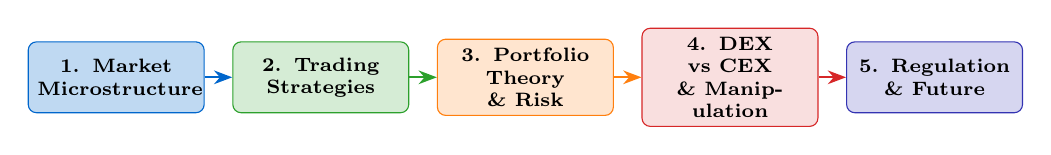
\begin{tikzpicture}[remember picture]
  \node[draw=mlblue, fill=mlblue!25, rounded corners=3pt, minimum width=2.1cm, minimum height=0.9cm, text width=2.0cm, align=center, font=\scriptsize\bfseries] (b1) {1. Market\\Microstructure};
  \node[draw=mlgreen, fill=mlgreen!20, rounded corners=3pt, minimum width=2.1cm, minimum height=0.9cm, text width=2.0cm, align=center, font=\scriptsize\bfseries, right=0.35cm of b1] (b2) {2. Trading\\Strategies};
  \node[draw=mlorange, fill=mlorange!20, rounded corners=3pt, minimum width=2.1cm, minimum height=0.9cm, text width=2.0cm, align=center, font=\scriptsize\bfseries, right=0.35cm of b2] (b3) {3. Portfolio\\Theory \& Risk};
  \node[draw=mlred, fill=mlred!15, rounded corners=3pt, minimum width=2.1cm, minimum height=0.9cm, text width=2.0cm, align=center, font=\scriptsize\bfseries, right=0.35cm of b3] (b4) {4. DEX vs CEX\\\& Manipulation};
  \node[draw=mlpurple, fill=mlpurple!20, rounded corners=3pt, minimum width=2.1cm, minimum height=0.9cm, text width=2.0cm, align=center, font=\scriptsize\bfseries, right=0.35cm of b4] (b5) {5. Regulation\\\& Future};
  \draw[-{Stealth}, thick, mlblue] (b1.east) -- (b2.west);
  \draw[-{Stealth}, thick, mlgreen] (b2.east) -- (b3.west);
  \draw[-{Stealth}, thick, mlorange] (b3.east) -- (b4.west);
  \draw[-{Stealth}, thick, mlred] (b4.east) -- (b5.west);
\end{tikzpicture}

\vspace{3mm}
\begin{columns}[T]
\column{0.5\textwidth}
\begin{block}{Learning Objectives}
\begin{itemize}\setlength{\itemsep}{1pt}
  \item Understand crypto market microstructure and order book mechanics
  \item Analyse quantitative trading strategies and their performance
  \item Apply modern portfolio theory and risk metrics to crypto assets
  \item Compare DEX and CEX architectures and detect manipulation
  \item Evaluate regulatory frameworks and their market impact
\end{itemize}
\end{block}
\column{0.5\textwidth}
\begin{block}{Prerequisites}
\begin{itemize}\setlength{\itemsep}{1pt}
  \item Blockchain fundamentals (Lessons 1--2)
  \item Smart contract basics (Lessons 3--4)
  \item DeFi protocols overview (Lesson 5)
  \item Basic statistics and probability
\end{itemize}
\end{block}
\end{columns}
\bottomnote{Duration: 90 minutes | 5 sections | \textasciitilde55 frames | Prerequisite: Lessons 1--5}
\end{frame}

% Frame 3: Table of Contents
\begin{frame}{Table of Contents}
\tableofcontents
\bottomnote{Navigate through 5 sections covering market microstructure to regulation and the future of crypto trading}
\end{frame}

\begin{frame}{Learning Objectives}
By the end of this lecture, you will be able to:
\begin{enumerate}
\item \textbf{Explain} order book mechanics (bid-ask spread, market depth, price discovery)
\item \textbf{Implement} and backtest basic trading strategies (momentum, mean reversion, arbitrage)
\item \textbf{Calculate} risk metrics (VaR, CVaR, Sharpe ratio, maximum drawdown) for crypto portfolios
\item \textbf{Compare} CEX and DEX architectures and their respective risk profiles
\item \textbf{Analyze} market manipulation techniques (wash trading, spoofing, front-running)
\end{enumerate}
\bottomnote{Bloom's taxonomy levels: Remember $\rightarrow$ Understand $\rightarrow$ Apply $\rightarrow$ Analyze $\rightarrow$ Evaluate $\rightarrow$ Create}
\end{frame}

%% ============================================================
%% SECTION 1: MARKET MICROSTRUCTURE & ORDER BOOKS
%% ============================================================
\section{Market Microstructure \& Order Books}

% Frame 4: Section 1 Divider
\begin{frame}{Section 1: Market Microstructure \& Order Books}
\begin{beamercolorbox}[sep=12pt,center,rounded=true,shadow=true]{palette quaternary}
  {\Large\bfseries Section 1: Market Microstructure \& Order Books}\\[4pt]
  {\normalsize Understanding how crypto markets operate at the granular level}
\end{beamercolorbox}

\vspace{4mm}
\begin{columns}[T]
\column{0.55\textwidth}
\begin{block}{What You Will Learn}
\begin{itemize}\setlength{\itemsep}{2pt}
  \item How centralised and decentralised exchanges structure their markets
  \item Order book anatomy: bids, asks, spread, and depth
  \item Order types and matching engine mechanics
  \item Price discovery, slippage, and market impact
  \item Fee structures across major exchanges
\end{itemize}
\end{block}
\column{0.45\textwidth}
\begin{block}{Frames in This Section}
\begin{itemize}\setlength{\itemsep}{2pt}
  \item Frame 5: The Crypto Trading Landscape
  \item Frame 6: Order Book Anatomy
  \item Frame 7: Order Types
  \item Frame 8: Order Matching Engine
  \item Frame 9: Bid-Ask Spread Analysis
  \item Frame 10: Market Depth \& Liquidity
  \item Frame 11: Price Discovery Mechanism
  \item Frame 12: Slippage and Market Impact
  \item Frame 13: Exchange Fee Structures
  \item Frame 14: Section 1 Summary
\end{itemize}
\end{block}
\end{columns}
\bottomnote{Section 1 of 5 | Frames 4--14 | Foundational market structure concepts before strategy deep dives}
\end{frame}

% Frame 5: The Crypto Trading Landscape
\begin{frame}{The Crypto Trading Landscape}
\begin{columns}[T]
\column{0.44\textwidth}
\begin{block}{Market Overview}
\begin{itemize}\setlength{\itemsep}{2pt}
  \item \textbf{24/7 markets:} Unlike equities, crypto trades around the clock with no closing bell
  \item \textbf{Global \& fragmented:} 500+ exchanges across jurisdictions with no consolidated tape
  \item \textbf{Daily volume:} \$50--150B spot; \$100--300B derivatives (2024 data)
  \item \textbf{Participants:} Retail, prop firms, market makers, miners, DeFi protocols
  \item \textbf{Asset classes:} Spot, perpetuals, options, tokenised assets, NFTs
\end{itemize}
\end{block}
\vspace{2mm}
\begin{alertblock}{Key Insight}
\scriptsize Crypto markets combine extreme fragmentation with 24/7 operation, creating unique microstructure dynamics unseen in traditional finance.
\end{alertblock}
\column{0.56\textwidth}
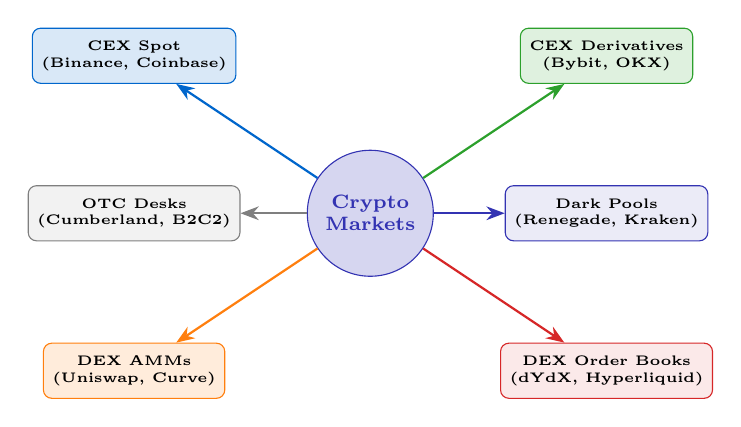
\begin{tikzpicture}
  % Central hub
  \node[draw=mlpurple, fill=mlpurple!20, circle, minimum size=1.6cm, font=\scriptsize\bfseries, align=center, text=mlpurple] (hub) at (3.5,3) {Crypto\\Markets};
  % Spokes
  \node[draw=mlblue, fill=mlblue!15, rounded corners=3pt, minimum width=2.0cm, minimum height=0.7cm, font=\tiny\bfseries, align=center] (s1) at (0.5,5.0) {CEX Spot\\(Binance, Coinbase)};
  \node[draw=mlgreen, fill=mlgreen!15, rounded corners=3pt, minimum width=2.0cm, minimum height=0.7cm, font=\tiny\bfseries, align=center] (s2) at (6.5,5.0) {CEX Derivatives\\(Bybit, OKX)};
  \node[draw=mlorange, fill=mlorange!15, rounded corners=3pt, minimum width=2.0cm, minimum height=0.7cm, font=\tiny\bfseries, align=center] (s3) at (0.5,1.0) {DEX AMMs\\(Uniswap, Curve)};
  \node[draw=mlred, fill=mlred!10, rounded corners=3pt, minimum width=2.0cm, minimum height=0.7cm, font=\tiny\bfseries, align=center] (s4) at (6.5,1.0) {DEX Order Books\\(dYdX, Hyperliquid)};
  \node[draw=mlgray, fill=mlgray!10, rounded corners=3pt, minimum width=2.0cm, minimum height=0.7cm, font=\tiny\bfseries, align=center] (s5) at (0.5,3.0) {OTC Desks\\(Cumberland, B2C2)};
  \node[draw=mlpurple, fill=mlpurple!10, rounded corners=3pt, minimum width=2.0cm, minimum height=0.7cm, font=\tiny\bfseries, align=center] (s6) at (6.5,3.0) {Dark Pools\\(Renegade, Kraken)};
  % Arrows
  \draw[-{Stealth}, thick, mlblue] (hub) -- (s1);
  \draw[-{Stealth}, thick, mlgreen] (hub) -- (s2);
  \draw[-{Stealth}, thick, mlorange] (hub) -- (s3);
  \draw[-{Stealth}, thick, mlred] (hub) -- (s4);
  \draw[-{Stealth}, thick, mlgray] (hub) -- (s5);
  \draw[-{Stealth}, thick, mlpurple] (hub) -- (s6);
\end{tikzpicture}
\end{columns}
\bottomnote{Crypto market structure: 500+ venues, \$50--300B daily volume, 24/7 operation | Fragmentation creates arbitrage but also risk}
\end{frame}

% Frame 6: Order Book Anatomy
\begin{frame}{Order Book Anatomy}
\adjustbox{max width=\textwidth, max totalheight=6.5cm}{%
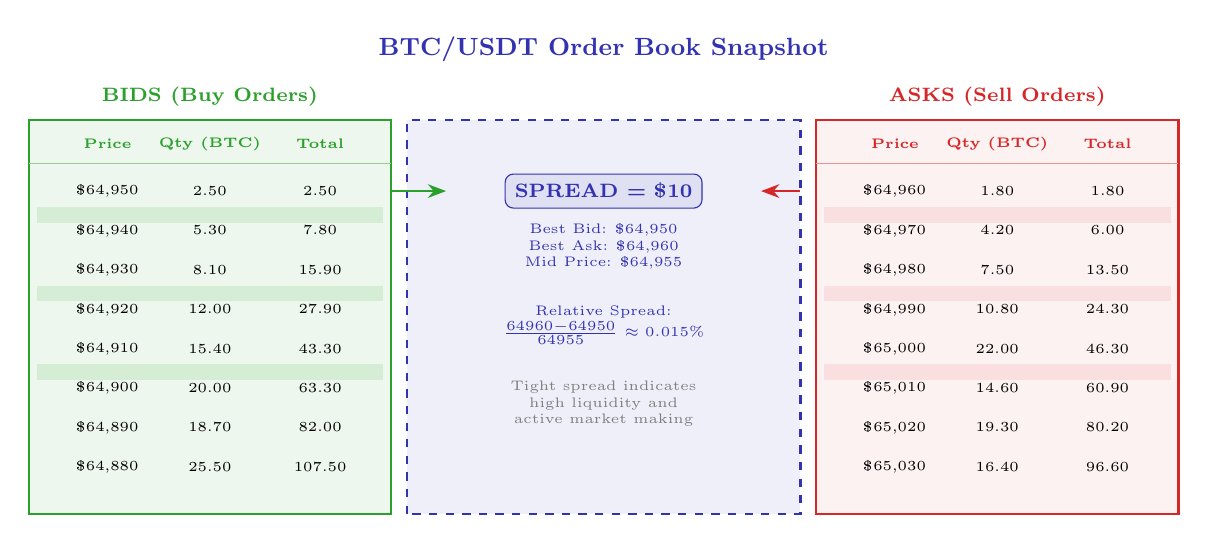
\begin{tikzpicture}
  % Title
  \node[font=\small\bfseries, text=mlpurple] at (7.5,6.3) {BTC/USDT Order Book Snapshot};

  % Bid side (left, green)
  \node[font=\scriptsize\bfseries, text=mlgreen] at (2.5,5.7) {BIDS (Buy Orders)};
  \fill[mlgreen!8] (0.2,0.4) rectangle (4.8,5.4);
  \draw[mlgreen, thick] (0.2,0.4) rectangle (4.8,5.4);

  % Bid headers
  \node[font=\tiny\bfseries, text=mlgreen] at (1.2,5.1) {Price};
  \node[font=\tiny\bfseries, text=mlgreen] at (2.5,5.1) {Qty (BTC)};
  \node[font=\tiny\bfseries, text=mlgreen] at (3.9,5.1) {Total};
  \draw[mlgreen!50] (0.2,4.85) -- (4.8,4.85);

  % Bid rows
  \node[font=\tiny] at (1.2,4.5) {\$64,950};
  \node[font=\tiny] at (2.5,4.5) {2.50};
  \node[font=\tiny] at (3.9,4.5) {2.50};
  \fill[mlgreen!20] (0.3,4.1) rectangle (4.7,4.3);
  \node[font=\tiny] at (1.2,4.0) {\$64,940};
  \node[font=\tiny] at (2.5,4.0) {5.30};
  \node[font=\tiny] at (3.9,4.0) {7.80};
  \node[font=\tiny] at (1.2,3.5) {\$64,930};
  \node[font=\tiny] at (2.5,3.5) {8.10};
  \node[font=\tiny] at (3.9,3.5) {15.90};
  \fill[mlgreen!20] (0.3,3.1) rectangle (4.7,3.3);
  \node[font=\tiny] at (1.2,3.0) {\$64,920};
  \node[font=\tiny] at (2.5,3.0) {12.00};
  \node[font=\tiny] at (3.9,3.0) {27.90};
  \node[font=\tiny] at (1.2,2.5) {\$64,910};
  \node[font=\tiny] at (2.5,2.5) {15.40};
  \node[font=\tiny] at (3.9,2.5) {43.30};
  \fill[mlgreen!20] (0.3,2.1) rectangle (4.7,2.3);
  \node[font=\tiny] at (1.2,2.0) {\$64,900};
  \node[font=\tiny] at (2.5,2.0) {20.00};
  \node[font=\tiny] at (3.9,2.0) {63.30};
  \node[font=\tiny] at (1.2,1.5) {\$64,890};
  \node[font=\tiny] at (2.5,1.5) {18.70};
  \node[font=\tiny] at (3.9,1.5) {82.00};
  \node[font=\tiny] at (1.2,1.0) {\$64,880};
  \node[font=\tiny] at (2.5,1.0) {25.50};
  \node[font=\tiny] at (3.9,1.0) {107.50};

  % Spread zone (center)
  \fill[mlpurple!8] (5.0,0.4) rectangle (10.0,5.4);
  \draw[mlpurple, thick, dashed] (5.0,0.4) rectangle (10.0,5.4);

  % Spread annotation
  \node[draw=mlpurple, fill=mlpurple!15, rounded corners=3pt, font=\scriptsize\bfseries, text=mlpurple, align=center, minimum width=2.5cm] at (7.5,4.5) {SPREAD = \$10};
  \node[font=\tiny, text=mlpurple, align=center] at (7.5,3.8) {Best Bid: \$64,950\\Best Ask: \$64,960\\Mid Price: \$64,955};
  \node[font=\tiny, text=mlpurple, align=center] at (7.5,2.8) {Relative Spread:\\$\frac{64960 - 64950}{64955} \approx 0.015\%$};
  \node[font=\tiny, text=mlgray, align=center] at (7.5,1.8) {Tight spread indicates\\high liquidity and\\active market making};
  \draw[-{Stealth}, thick, mlgreen] (4.8,4.5) -- (5.5,4.5);
  \draw[-{Stealth}, thick, mlred] (10.0,4.5) -- (9.5,4.5);

  % Ask side (right, red)
  \node[font=\scriptsize\bfseries, text=mlred] at (12.5,5.7) {ASKS (Sell Orders)};
  \fill[mlred!6] (10.2,0.4) rectangle (14.8,5.4);
  \draw[mlred, thick] (10.2,0.4) rectangle (14.8,5.4);

  % Ask headers
  \node[font=\tiny\bfseries, text=mlred] at (11.2,5.1) {Price};
  \node[font=\tiny\bfseries, text=mlred] at (12.5,5.1) {Qty (BTC)};
  \node[font=\tiny\bfseries, text=mlred] at (13.9,5.1) {Total};
  \draw[mlred!50] (10.2,4.85) -- (14.8,4.85);

  % Ask rows
  \node[font=\tiny] at (11.2,4.5) {\$64,960};
  \node[font=\tiny] at (12.5,4.5) {1.80};
  \node[font=\tiny] at (13.9,4.5) {1.80};
  \fill[mlred!15] (10.3,4.1) rectangle (14.7,4.3);
  \node[font=\tiny] at (11.2,4.0) {\$64,970};
  \node[font=\tiny] at (12.5,4.0) {4.20};
  \node[font=\tiny] at (13.9,4.0) {6.00};
  \node[font=\tiny] at (11.2,3.5) {\$64,980};
  \node[font=\tiny] at (12.5,3.5) {7.50};
  \node[font=\tiny] at (13.9,3.5) {13.50};
  \fill[mlred!15] (10.3,3.1) rectangle (14.7,3.3);
  \node[font=\tiny] at (11.2,3.0) {\$64,990};
  \node[font=\tiny] at (12.5,3.0) {10.80};
  \node[font=\tiny] at (13.9,3.0) {24.30};
  \node[font=\tiny] at (11.2,2.5) {\$65,000};
  \node[font=\tiny] at (12.5,2.5) {22.00};
  \node[font=\tiny] at (13.9,2.5) {46.30};
  \fill[mlred!15] (10.3,2.1) rectangle (14.7,2.3);
  \node[font=\tiny] at (11.2,2.0) {\$65,010};
  \node[font=\tiny] at (12.5,2.0) {14.60};
  \node[font=\tiny] at (13.9,2.0) {60.90};
  \node[font=\tiny] at (11.2,1.5) {\$65,020};
  \node[font=\tiny] at (12.5,1.5) {19.30};
  \node[font=\tiny] at (13.9,1.5) {80.20};
  \node[font=\tiny] at (11.2,1.0) {\$65,030};
  \node[font=\tiny] at (12.5,1.0) {16.40};
  \node[font=\tiny] at (13.9,1.0) {96.60};
\end{tikzpicture}%
}%
\bottomnote{Order book = central data structure of all exchanges | Green bids (buy) vs red asks (sell) | Spread = best ask $-$ best bid}
\end{frame}

% Frame 7: Order Types
\begin{frame}{Order Types in Crypto Markets}
\adjustbox{max width=\textwidth}{%
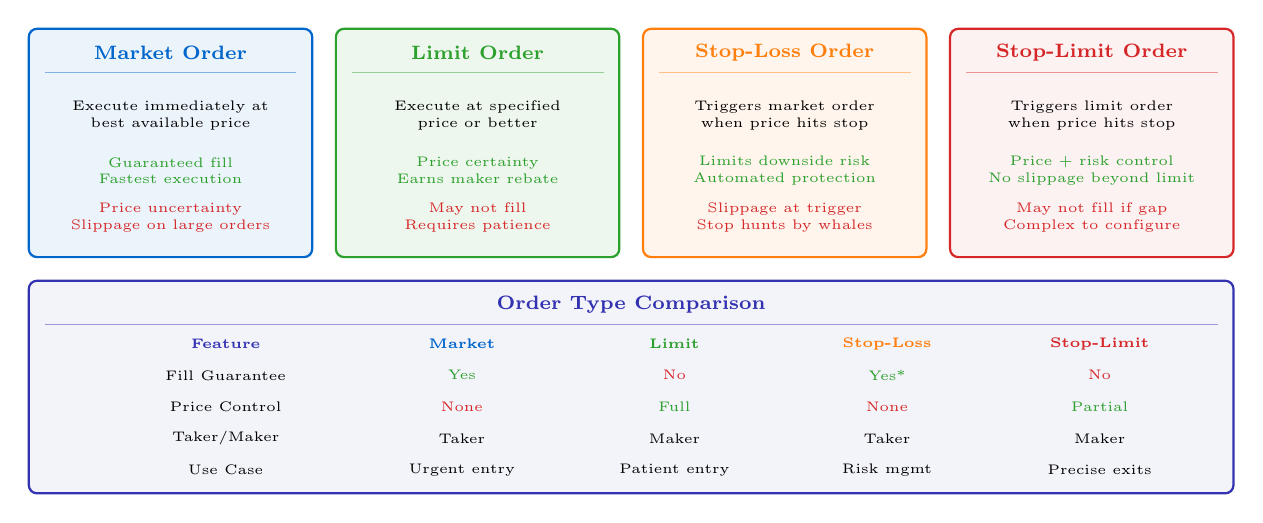
\begin{tikzpicture}
  % Panel 1: Market Order
  \fill[mlblue!8] (0,3.3) rectangle (3.6,6.2);
  \draw[mlblue, thick, rounded corners=3pt] (0,3.3) rectangle (3.6,6.2);
  \node[font=\scriptsize\bfseries, text=mlblue] at (1.8,5.9) {Market Order};
  \draw[mlblue!50] (0.2,5.65) -- (3.4,5.65);
  \node[font=\tiny, align=center, text width=3.2cm] at (1.8,5.1) {Execute immediately at\\best available price};
  \node[font=\tiny, align=center, text width=3.2cm, text=mlgreen] at (1.8,4.4) {Guaranteed fill\\Fastest execution};
  \node[font=\tiny, align=center, text width=3.2cm, text=mlred] at (1.8,3.8) {Price uncertainty\\Slippage on large orders};

  % Panel 2: Limit Order
  \fill[mlgreen!8] (3.9,3.3) rectangle (7.5,6.2);
  \draw[mlgreen, thick, rounded corners=3pt] (3.9,3.3) rectangle (7.5,6.2);
  \node[font=\scriptsize\bfseries, text=mlgreen] at (5.7,5.9) {Limit Order};
  \draw[mlgreen!50] (4.1,5.65) -- (7.3,5.65);
  \node[font=\tiny, align=center, text width=3.2cm] at (5.7,5.1) {Execute at specified\\price or better};
  \node[font=\tiny, align=center, text width=3.2cm, text=mlgreen] at (5.7,4.4) {Price certainty\\Earns maker rebate};
  \node[font=\tiny, align=center, text width=3.2cm, text=mlred] at (5.7,3.8) {May not fill\\Requires patience};

  % Panel 3: Stop-Loss Order
  \fill[mlorange!8] (7.8,3.3) rectangle (11.4,6.2);
  \draw[mlorange, thick, rounded corners=3pt] (7.8,3.3) rectangle (11.4,6.2);
  \node[font=\scriptsize\bfseries, text=mlorange] at (9.6,5.9) {Stop-Loss Order};
  \draw[mlorange!50] (8.0,5.65) -- (11.2,5.65);
  \node[font=\tiny, align=center, text width=3.2cm] at (9.6,5.1) {Triggers market order\\when price hits stop};
  \node[font=\tiny, align=center, text width=3.2cm, text=mlgreen] at (9.6,4.4) {Limits downside risk\\Automated protection};
  \node[font=\tiny, align=center, text width=3.2cm, text=mlred] at (9.6,3.8) {Slippage at trigger\\Stop hunts by whales};

  % Panel 4: Stop-Limit Order
  \fill[mlred!6] (11.7,3.3) rectangle (15.3,6.2);
  \draw[mlred, thick, rounded corners=3pt] (11.7,3.3) rectangle (15.3,6.2);
  \node[font=\scriptsize\bfseries, text=mlred] at (13.5,5.9) {Stop-Limit Order};
  \draw[mlred!50] (11.9,5.65) -- (15.1,5.65);
  \node[font=\tiny, align=center, text width=3.2cm] at (13.5,5.1) {Triggers limit order\\when price hits stop};
  \node[font=\tiny, align=center, text width=3.2cm, text=mlgreen] at (13.5,4.4) {Price + risk control\\No slippage beyond limit};
  \node[font=\tiny, align=center, text width=3.2cm, text=mlred] at (13.5,3.8) {May not fill if gap\\Complex to configure};

  % Comparison row
  \fill[mlpurple!6] (0,0.3) rectangle (15.3,3.0);
  \draw[mlpurple, thick, rounded corners=3pt] (0,0.3) rectangle (15.3,3.0);
  \node[font=\scriptsize\bfseries, text=mlpurple] at (7.65,2.7) {Order Type Comparison};
  \draw[mlpurple!50] (0.2,2.45) -- (15.1,2.45);

  % Table headers
  \node[font=\tiny\bfseries, text=mlpurple] at (2.5,2.2) {Feature};
  \node[font=\tiny\bfseries, text=mlblue] at (5.5,2.2) {Market};
  \node[font=\tiny\bfseries, text=mlgreen] at (8.2,2.2) {Limit};
  \node[font=\tiny\bfseries, text=mlorange] at (10.9,2.2) {Stop-Loss};
  \node[font=\tiny\bfseries, text=mlred] at (13.6,2.2) {Stop-Limit};

  \node[font=\tiny] at (2.5,1.8) {Fill Guarantee};
  \node[font=\tiny, text=mlgreen] at (5.5,1.8) {Yes};
  \node[font=\tiny, text=mlred] at (8.2,1.8) {No};
  \node[font=\tiny, text=mlgreen] at (10.9,1.8) {Yes*};
  \node[font=\tiny, text=mlred] at (13.6,1.8) {No};

  \node[font=\tiny] at (2.5,1.4) {Price Control};
  \node[font=\tiny, text=mlred] at (5.5,1.4) {None};
  \node[font=\tiny, text=mlgreen] at (8.2,1.4) {Full};
  \node[font=\tiny, text=mlred] at (10.9,1.4) {None};
  \node[font=\tiny, text=mlgreen] at (13.6,1.4) {Partial};

  \node[font=\tiny] at (2.5,1.0) {Taker/Maker};
  \node[font=\tiny] at (5.5,1.0) {Taker};
  \node[font=\tiny] at (8.2,1.0) {Maker};
  \node[font=\tiny] at (10.9,1.0) {Taker};
  \node[font=\tiny] at (13.6,1.0) {Maker};

  \node[font=\tiny] at (2.5,0.6) {Use Case};
  \node[font=\tiny] at (5.5,0.6) {Urgent entry};
  \node[font=\tiny] at (8.2,0.6) {Patient entry};
  \node[font=\tiny] at (10.9,0.6) {Risk mgmt};
  \node[font=\tiny] at (13.6,0.6) {Precise exits};
\end{tikzpicture}%
}%
\bottomnote{Order types: market (immediate, taker), limit (patient, maker), stop-loss (protection), stop-limit (precise protection) | *Stop-loss fills as market order --- slippage possible}
\end{frame}

% Frame 8: Order Matching Engine [FRAGILE] -- CODE FRAME 1
\begin{frame}[fragile]{Order Matching Engine}
\begin{columns}[T]
\column{0.50\textwidth}
\begin{lstlisting}[language=Python, caption={Price-Time Priority Matching}]
# Simple Order Matching Engine
def match_orders(order_book):
    while order_book.has_match():
        best_bid = order_book.top_bid()
        best_ask = order_book.top_ask()

        if best_bid.price >= best_ask.price:
            qty = min(best_bid.qty,
                      best_ask.qty)
            execute_trade(
                price=best_ask.price,
                quantity=qty)
            update_book(best_bid, best_ask,
                        qty)
        else:
            break  # no more matches
\end{lstlisting}
\vspace{1mm}
\begin{alertblock}{Key Principle}
\scriptsize Trades execute at the \textbf{ask price} (price of the passive order). The aggressor (taker) crosses the spread.
\end{alertblock}
\column{0.50\textwidth}
\begin{block}{Price-Time Priority}
\begin{itemize}\setlength{\itemsep}{2pt}
  \item \textbf{Step 1:} Sort bids descending, asks ascending by price
  \item \textbf{Step 2:} Match highest bid against lowest ask
  \item \textbf{Step 3:} If bid $\geq$ ask, a trade occurs
  \item \textbf{Step 4:} Fill at the \emph{passive} side's price
  \item \textbf{Step 5:} Among equal prices, first-in-first-out (FIFO)
\end{itemize}
\end{block}
\vspace{2mm}
\begin{block}{Matching Engine Properties}
\begin{itemize}\setlength{\itemsep}{2pt}
  \item \textbf{Latency:} Top CEXs match in $<$1ms; Binance $\approx$5$\mu$s
  \item \textbf{Throughput:} 100K--1M orders/second
  \item \textbf{Fairness:} FIFO prevents front-running at same price level
  \item \textbf{Partial fills:} Large orders matched incrementally across multiple counterparties
  \item \textbf{DEX difference:} AMMs replace order books with $x \cdot y = k$ invariant
\end{itemize}
\end{block}
\end{columns}
\bottomnote{Price-time priority: standard matching algorithm for CEXs | Execution at passive price | FIFO among equal-price orders | DEXs use AMM curves instead}
\end{frame}

% Frame 9: Bid-Ask Spread Analysis
\begin{frame}{Bid-Ask Spread Analysis}
\begin{columns}[T]
\column{0.44\textwidth}
\begin{block}{Spread Definitions}
\begin{itemize}\setlength{\itemsep}{2pt}
  \item \textbf{Absolute spread:} $S = P_a - P_b$
  \item \textbf{Relative spread:} $S_r = \frac{P_a - P_b}{P_m}$ where $P_m = \frac{P_a + P_b}{2}$
  \item \textbf{Effective spread:} $S_e = 2 \cdot |P_{\text{trade}} - P_m|$
  \item \textbf{Realized spread:} $S_{\text{real}} = 2 \cdot (P_{\text{trade}} - P_{m,t+\Delta t})$
\end{itemize}
\end{block}
\vspace{1mm}
\begin{block}{Spread Determinants}
\begin{itemize}\setlength{\itemsep}{1pt}
  \item \textbf{Volatility:} Higher vol $\Rightarrow$ wider spread (adverse selection)
  \item \textbf{Volume:} More activity $\Rightarrow$ tighter spread
  \item \textbf{Competition:} More market makers $\Rightarrow$ tighter spread
  \item \textbf{Tick size:} Minimum price increment constrains spread
  \item \textbf{Information:} Informed flow widens spread
\end{itemize}
\end{block}
\column{0.56\textwidth}
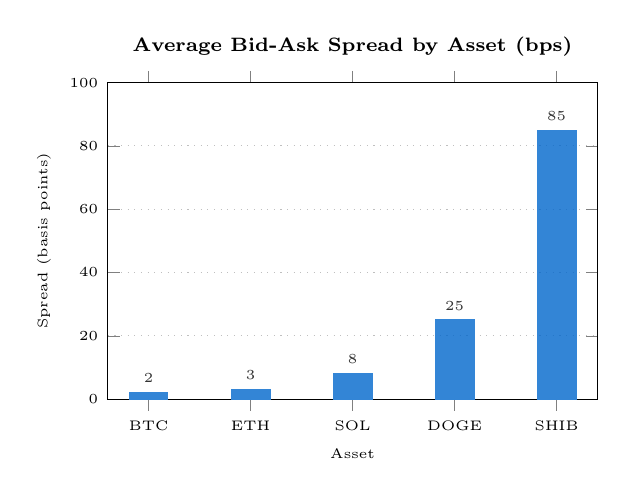
\begin{tikzpicture}
\begin{axis}[
  width=7.8cm, height=5.6cm,
  title={\scriptsize\bfseries Average Bid-Ask Spread by Asset (bps)},
  xlabel={\tiny Asset},
  ylabel={\tiny Spread (basis points)},
  ymin=0, ymax=100,
  symbolic x coords={BTC,ETH,SOL,DOGE,SHIB},
  xtick=data,
  x tick label style={font=\tiny},
  y tick label style={font=\tiny},
  ybar,
  bar width=14pt,
  nodes near coords,
  nodes near coords style={font=\tiny\bfseries},
  every axis plot/.append style={fill opacity=0.8},
  ymajorgrids=true,
  grid style={dotted, mlgray!50},
  legend style={font=\tiny, at={(0.97,0.97)}, anchor=north east}
]
\addplot[fill=mlblue, draw=mlblue!80] coordinates {(BTC,2) (ETH,3) (SOL,8) (DOGE,25) (SHIB,85)};
\end{axis}
\end{tikzpicture}
\vspace{1mm}
\begin{alertblock}{Stylised Fact}
\scriptsize Spreads scale inversely with market cap and volume. BTC spread $\approx$0.02\%; micro-caps can exceed 1\%. This cost is invisible but significant for active traders.
\end{alertblock}
\end{columns}
\bottomnote{Spread = implicit trading cost | BTC: $\sim$2 bps, micro-caps: $>$100 bps | Determinants: volatility, volume, competition, information asymmetry}
\end{frame}

% Frame 10: Market Depth & Liquidity
\begin{frame}{Market Depth \& Liquidity}
\begin{columns}[T]
\column{0.50\textwidth}
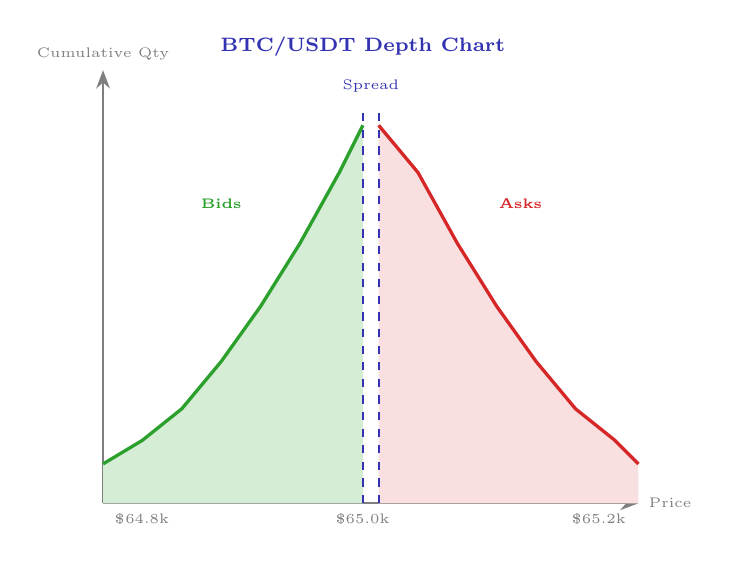
\begin{tikzpicture}
  \node[font=\scriptsize\bfseries, text=mlpurple] at (3.3,5.8) {BTC/USDT Depth Chart};

  % Axes
  \draw[-{Stealth}, thick, mlgray] (0,0) -- (6.8,0) node[right, font=\tiny] {Price};
  \draw[-{Stealth}, thick, mlgray] (0,0) -- (0,5.5) node[above, font=\tiny] {Cumulative Qty};

  % Bid curve (green, left side)
  \fill[mlgreen!20] (0,0) -- (0,0.5) -- (0.5,0.8) -- (1.0,1.2) -- (1.5,1.8) -- (2.0,2.5) -- (2.5,3.3) -- (3.0,4.2) -- (3.3,4.8) -- (3.3,0) -- cycle;
  \draw[mlgreen, very thick] (0,0.5) -- (0.5,0.8) -- (1.0,1.2) -- (1.5,1.8) -- (2.0,2.5) -- (2.5,3.3) -- (3.0,4.2) -- (3.3,4.8);
  \node[font=\tiny\bfseries, text=mlgreen] at (1.5,3.8) {Bids};

  % Ask curve (red, right side)
  \fill[mlred!15] (3.5,4.8) -- (4.0,4.2) -- (4.5,3.3) -- (5.0,2.5) -- (5.5,1.8) -- (6.0,1.2) -- (6.5,0.8) -- (6.8,0.5) -- (6.8,0) -- (3.5,0) -- cycle;
  \draw[mlred, very thick] (3.5,4.8) -- (4.0,4.2) -- (4.5,3.3) -- (5.0,2.5) -- (5.5,1.8) -- (6.0,1.2) -- (6.5,0.8) -- (6.8,0.5);
  \node[font=\tiny\bfseries, text=mlred] at (5.3,3.8) {Asks};

  % Spread zone
  \draw[mlpurple, thick, dashed] (3.3,0) -- (3.3,5.0);
  \draw[mlpurple, thick, dashed] (3.5,0) -- (3.5,5.0);
  \node[font=\tiny, text=mlpurple, align=center] at (3.4,5.3) {Spread};

  % Price labels
  \node[font=\tiny, text=mlgray] at (0.5,0) [below] {\$64.8k};
  \node[font=\tiny, text=mlgray] at (3.3,0) [below] {\$65.0k};
  \node[font=\tiny, text=mlgray] at (6.3,0) [below] {\$65.2k};
\end{tikzpicture}
\column{0.50\textwidth}
\begin{block}{Liquidity Metrics}
\begin{itemize}\setlength{\itemsep}{2pt}
  \item \textbf{Depth at $\pm$2\%:} Total volume within 2\% of mid-price; BTC: \$50--100M on Binance
  \item \textbf{Kyle's Lambda ($\lambda$):}
  \[\Delta P = \lambda \cdot Q + \epsilon\]
  Price impact per unit of order flow
  \item \textbf{Amihud Illiquidity:}
  \[ILLIQ = \frac{|r_t|}{V_t}\]
  Daily absolute return divided by volume
  \item \textbf{Order-to-trade ratio:} Measures market maker activity; typically 10--50$\times$ in crypto
\end{itemize}
\end{block}
\vspace{1mm}
\begin{alertblock}{Liquidity Mirage}
\scriptsize Crypto depth can vanish in seconds during volatile events. The March 2020 crash saw Binance BTC depth drop 80\% in minutes as market makers pulled quotes.
\end{alertblock}
\end{columns}
\bottomnote{Depth chart: cumulative bids (green) vs asks (red) | Key metrics: depth at $\pm$2\%, Kyle's $\lambda$, Amihud ILLIQ | Liquidity can evaporate rapidly in stress}
\end{frame}

% Frame 11: Price Discovery Mechanism
\begin{frame}{Price Discovery Mechanism}
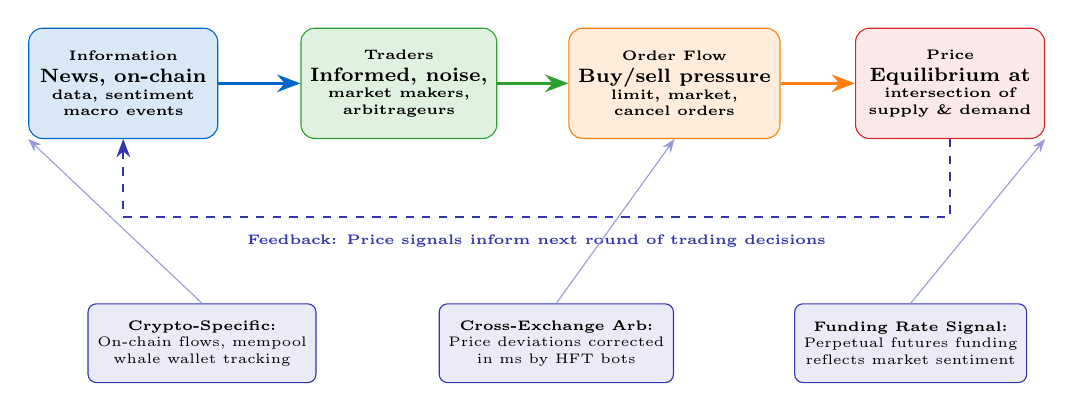
\begin{tikzpicture}
  % Flow: Information -> Traders -> Orders -> Price -> Consensus
  \node[draw=mlblue, fill=mlblue!15, rounded corners=5pt, minimum width=2.4cm, minimum height=1.4cm, align=center, font=\tiny\bfseries] (info) at (1.5,4.5) {Information\\[2pt]\scriptsize News, on-chain\\data, sentiment\\macro events};

  \node[draw=mlgreen, fill=mlgreen!15, rounded corners=5pt, minimum width=2.4cm, minimum height=1.4cm, align=center, font=\tiny\bfseries] (traders) at (5.0,4.5) {Traders\\[2pt]\scriptsize Informed, noise,\\market makers,\\arbitrageurs};

  \node[draw=mlorange, fill=mlorange!15, rounded corners=5pt, minimum width=2.4cm, minimum height=1.4cm, align=center, font=\tiny\bfseries] (orders) at (8.5,4.5) {Order Flow\\[2pt]\scriptsize Buy/sell pressure\\limit, market,\\cancel orders};

  \node[draw=mlred, fill=mlred!10, rounded corners=5pt, minimum width=2.4cm, minimum height=1.4cm, align=center, font=\tiny\bfseries] (price) at (12.0,4.5) {Price\\[2pt]\scriptsize Equilibrium at\\intersection of\\supply \& demand};

  % Arrows between main flow
  \draw[-{Stealth}, very thick, mlblue] (info.east) -- (traders.west);
  \draw[-{Stealth}, very thick, mlgreen] (traders.east) -- (orders.west);
  \draw[-{Stealth}, very thick, mlorange] (orders.east) -- (price.west);

  % Feedback loop
  \draw[-{Stealth}, thick, mlpurple, dashed] (price.south) -- (12.0,2.8) -- (1.5,2.8) -- (info.south);
  \node[font=\tiny\bfseries, text=mlpurple] at (6.75,2.5) {Feedback: Price signals inform next round of trading decisions};

  % Crypto-specific elements
  \node[draw=mlpurple, fill=mlpurple!10, rounded corners=3pt, minimum width=2.8cm, minimum height=1.0cm, align=center, font=\tiny] (crypto1) at (2.5,1.2) {\textbf{Crypto-Specific:}\\On-chain flows, mempool\\whale wallet tracking};

  \node[draw=mlpurple, fill=mlpurple!10, rounded corners=3pt, minimum width=2.8cm, minimum height=1.0cm, align=center, font=\tiny] (crypto2) at (7.0,1.2) {\textbf{Cross-Exchange Arb:}\\Price deviations corrected\\in ms by HFT bots};

  \node[draw=mlpurple, fill=mlpurple!10, rounded corners=3pt, minimum width=2.8cm, minimum height=1.0cm, align=center, font=\tiny] (crypto3) at (11.5,1.2) {\textbf{Funding Rate Signal:}\\Perpetual futures funding\\reflects market sentiment};

  \draw[-{Stealth}, thin, mlpurple!50] (crypto1.north) -- (info.south west);
  \draw[-{Stealth}, thin, mlpurple!50] (crypto2.north) -- (orders.south);
  \draw[-{Stealth}, thin, mlpurple!50] (crypto3.north) -- (price.south east);
\end{tikzpicture}
\bottomnote{Price discovery: information $\to$ traders $\to$ order flow $\to$ price equilibrium $\to$ feedback | Crypto-specific: on-chain data, cross-exchange arbitrage, funding rates}
\end{frame}

% Frame 12: Slippage and Market Impact
\begin{frame}{Slippage and Market Impact}
\begin{columns}[T]
\column{0.48\textwidth}
\begin{block}{Slippage Defined}
\begin{itemize}\setlength{\itemsep}{2pt}
  \item \textbf{Slippage} = difference between expected and actual execution price
  \item Caused by consuming multiple price levels in the order book
  \item $\text{Slippage} = \frac{P_{\text{avg}} - P_{\text{best}}}{P_{\text{best}}} \times 100\%$
\end{itemize}
\end{block}
\vspace{2mm}
\begin{block}{Market Impact Models}
\begin{itemize}\setlength{\itemsep}{2pt}
  \item \textbf{Square-root law} (empirical):
  \[\Delta P \approx \sigma \cdot \sqrt{\frac{Q}{V}}\]
  where $\sigma$ = volatility, $Q$ = order size, $V$ = daily volume
  \item \textbf{Almgren-Chriss:} Optimal execution minimises impact + risk trade-off
  \item \textbf{Crypto twist:} Fragmented liquidity across exchanges magnifies impact
\end{itemize}
\end{block}
\column{0.52\textwidth}
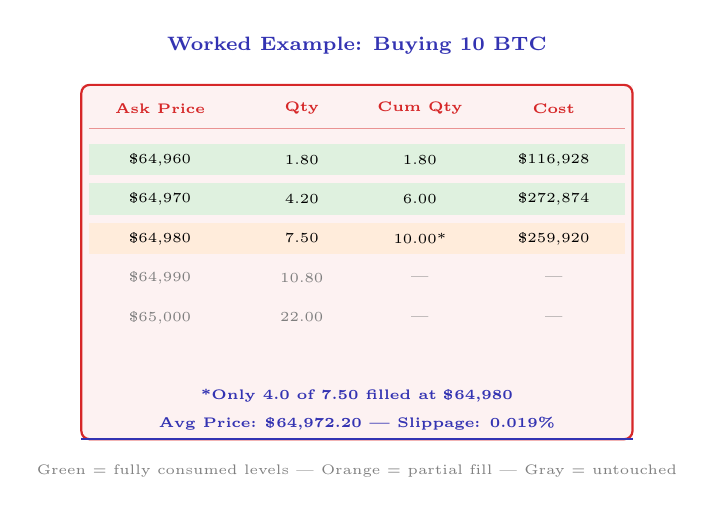
\begin{tikzpicture}
  \node[font=\scriptsize\bfseries, text=mlpurple] at (4.0,6.0) {Worked Example: Buying 10 BTC};

  % Order book representation
  \fill[mlred!6] (0.5,1.0) rectangle (7.5,5.5);
  \draw[mlred, thick, rounded corners=3pt] (0.5,1.0) rectangle (7.5,5.5);

  % Headers
  \node[font=\tiny\bfseries, text=mlred] at (1.5,5.2) {Ask Price};
  \node[font=\tiny\bfseries, text=mlred] at (3.3,5.2) {Qty};
  \node[font=\tiny\bfseries, text=mlred] at (4.8,5.2) {Cum Qty};
  \node[font=\tiny\bfseries, text=mlred] at (6.5,5.2) {Cost};
  \draw[mlred!50] (0.6,4.95) -- (7.4,4.95);

  % Row 1 - filled
  \fill[mlgreen!15] (0.6,4.35) rectangle (7.4,4.75);
  \node[font=\tiny] at (1.5,4.55) {\$64,960};
  \node[font=\tiny] at (3.3,4.55) {1.80};
  \node[font=\tiny] at (4.8,4.55) {1.80};
  \node[font=\tiny] at (6.5,4.55) {\$116,928};

  % Row 2 - filled
  \fill[mlgreen!15] (0.6,3.85) rectangle (7.4,4.25);
  \node[font=\tiny] at (1.5,4.05) {\$64,970};
  \node[font=\tiny] at (3.3,4.05) {4.20};
  \node[font=\tiny] at (4.8,4.05) {6.00};
  \node[font=\tiny] at (6.5,4.05) {\$272,874};

  % Row 3 - partially filled
  \fill[mlorange!15] (0.6,3.35) rectangle (7.4,3.75);
  \node[font=\tiny] at (1.5,3.55) {\$64,980};
  \node[font=\tiny] at (3.3,3.55) {7.50};
  \node[font=\tiny] at (4.8,3.55) {10.00*};
  \node[font=\tiny] at (6.5,3.55) {\$259,920};

  % Remaining rows
  \node[font=\tiny, text=mlgray] at (1.5,3.05) {\$64,990};
  \node[font=\tiny, text=mlgray] at (3.3,3.05) {10.80};
  \node[font=\tiny, text=mlgray] at (4.8,3.05) {---};
  \node[font=\tiny, text=mlgray] at (6.5,3.05) {---};
  \node[font=\tiny, text=mlgray] at (1.5,2.55) {\$65,000};
  \node[font=\tiny, text=mlgray] at (3.3,2.55) {22.00};
  \node[font=\tiny, text=mlgray] at (4.8,2.55) {---};
  \node[font=\tiny, text=mlgray] at (6.5,2.55) {---};

  % Summary
  \draw[mlpurple, thick] (0.5,1.0) -- (7.5,1.0);
  \node[font=\tiny\bfseries, text=mlpurple, align=center] at (4.0,1.55) {*Only 4.0 of 7.50 filled at \$64,980};
  \node[font=\tiny\bfseries, text=mlpurple, align=center] at (4.0,1.2) {Avg Price: \$64,972.20 | Slippage: 0.019\%};

  % Annotation
  \node[font=\tiny, text=mlgray, align=center] at (4.0,0.6) {Green = fully consumed levels | Orange = partial fill | Gray = untouched};
\end{tikzpicture}
\end{columns}
\bottomnote{Slippage: market orders consume multiple levels | Square-root impact law: $\Delta P \propto \sigma\sqrt{Q/V}$ | 10 BTC order: 0.019\% slippage across 3 price levels}
\end{frame}

% Frame 13: Exchange Fee Structures
\begin{frame}{Exchange Fee Structures}
\adjustbox{max width=\textwidth, max totalheight=6.5cm}{%
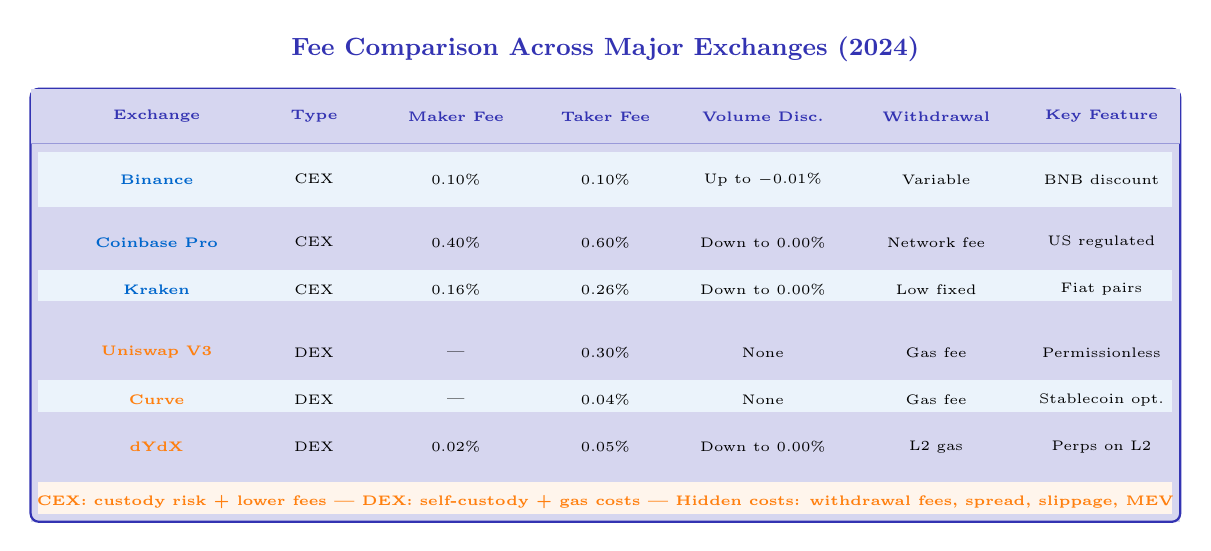
\begin{tikzpicture}
  \node[font=\small\bfseries, text=mlpurple] at (7.5,6.3) {Fee Comparison Across Major Exchanges (2024)};

  % Table background
  \fill[mllavender4] (0.2,0.3) rectangle (14.8,5.8);
  \draw[mlpurple, thick, rounded corners=3pt] (0.2,0.3) rectangle (14.8,5.8);

  % Header row
  \fill[mlpurple!20] (0.2,5.1) rectangle (14.8,5.8);
  \node[font=\tiny\bfseries, text=mlpurple] at (1.8,5.45) {Exchange};
  \node[font=\tiny\bfseries, text=mlpurple] at (3.8,5.45) {Type};
  \node[font=\tiny\bfseries, text=mlpurple] at (5.6,5.45) {Maker Fee};
  \node[font=\tiny\bfseries, text=mlpurple] at (7.5,5.45) {Taker Fee};
  \node[font=\tiny\bfseries, text=mlpurple] at (9.5,5.45) {Volume Disc.};
  \node[font=\tiny\bfseries, text=mlpurple] at (11.7,5.45) {Withdrawal};
  \node[font=\tiny\bfseries, text=mlpurple] at (13.8,5.45) {Key Feature};
  \draw[mlpurple!50] (0.2,5.1) -- (14.8,5.1);

  % Binance
  \fill[mlblue!8] (0.3,4.3) rectangle (14.7,5.0);
  \node[font=\tiny\bfseries, text=mlblue] at (1.8,4.65) {Binance};
  \node[font=\tiny] at (3.8,4.65) {CEX};
  \node[font=\tiny] at (5.6,4.65) {0.10\%};
  \node[font=\tiny] at (7.5,4.65) {0.10\%};
  \node[font=\tiny] at (9.5,4.65) {Up to $-$0.01\%};
  \node[font=\tiny] at (11.7,4.65) {Variable};
  \node[font=\tiny] at (13.8,4.65) {BNB discount};

  % Coinbase
  \node[font=\tiny\bfseries, text=mlblue] at (1.8,3.85) {Coinbase Pro};
  \node[font=\tiny] at (3.8,3.85) {CEX};
  \node[font=\tiny] at (5.6,3.85) {0.40\%};
  \node[font=\tiny] at (7.5,3.85) {0.60\%};
  \node[font=\tiny] at (9.5,3.85) {Down to 0.00\%};
  \node[font=\tiny] at (11.7,3.85) {Network fee};
  \node[font=\tiny] at (13.8,3.85) {US regulated};

  % Kraken
  \fill[mlblue!8] (0.3,3.1) rectangle (14.7,3.5);
  \node[font=\tiny\bfseries, text=mlblue] at (1.8,3.25) {Kraken};
  \node[font=\tiny] at (3.8,3.25) {CEX};
  \node[font=\tiny] at (5.6,3.25) {0.16\%};
  \node[font=\tiny] at (7.5,3.25) {0.26\%};
  \node[font=\tiny] at (9.5,3.25) {Down to 0.00\%};
  \node[font=\tiny] at (11.7,3.25) {Low fixed};
  \node[font=\tiny] at (13.8,3.25) {Fiat pairs};

  % Uniswap
  \node[font=\tiny\bfseries, text=mlorange] at (1.8,2.45) {Uniswap V3};
  \node[font=\tiny] at (3.8,2.45) {DEX};
  \node[font=\tiny] at (5.6,2.45) {---};
  \node[font=\tiny] at (7.5,2.45) {0.30\%};
  \node[font=\tiny] at (9.5,2.45) {None};
  \node[font=\tiny] at (11.7,2.45) {Gas fee};
  \node[font=\tiny] at (13.8,2.45) {Permissionless};

  % Curve
  \fill[mlblue!8] (0.3,1.7) rectangle (14.7,2.1);
  \node[font=\tiny\bfseries, text=mlorange] at (1.8,1.85) {Curve};
  \node[font=\tiny] at (3.8,1.85) {DEX};
  \node[font=\tiny] at (5.6,1.85) {---};
  \node[font=\tiny] at (7.5,1.85) {0.04\%};
  \node[font=\tiny] at (9.5,1.85) {None};
  \node[font=\tiny] at (11.7,1.85) {Gas fee};
  \node[font=\tiny] at (13.8,1.85) {Stablecoin opt.};

  % dYdX
  \node[font=\tiny\bfseries, text=mlorange] at (1.8,1.25) {dYdX};
  \node[font=\tiny] at (3.8,1.25) {DEX};
  \node[font=\tiny] at (5.6,1.25) {0.02\%};
  \node[font=\tiny] at (7.5,1.25) {0.05\%};
  \node[font=\tiny] at (9.5,1.25) {Down to 0.00\%};
  \node[font=\tiny] at (11.7,1.25) {L2 gas};
  \node[font=\tiny] at (13.8,1.25) {Perps on L2};

  % Annotations
  \fill[mlorange!8] (0.3,0.4) rectangle (14.7,0.8);
  \node[font=\tiny\bfseries, text=mlorange, align=center] at (7.5,0.55) {CEX: custody risk + lower fees | DEX: self-custody + gas costs | Hidden costs: withdrawal fees, spread, slippage, MEV};
\end{tikzpicture}%
}%
\bottomnote{Fee comparison: Binance (0.10\%), Coinbase (0.60\%), Uniswap (0.30\%), Curve (0.04\%) | Always consider total cost: fees + spread + slippage + gas}
\end{frame}

% Frame 14: Section 1 Summary
\begin{frame}{Section 1 Summary}
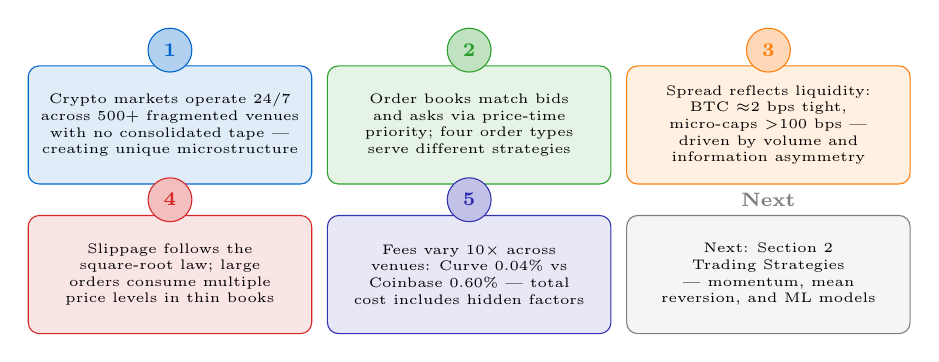
\begin{tikzpicture}
  \node[draw=mlblue, fill=mlblue!12, rounded corners=4pt, minimum width=3.6cm, minimum height=1.5cm, align=center, font=\tiny] (k1) at (1.9,3.2) {Crypto markets operate 24/7\\across 500+ fragmented venues\\with no consolidated tape ---\\creating unique microstructure};
  \node[circle, draw=mlblue, fill=mlblue!30, minimum size=0.55cm, font=\scriptsize\bfseries, text=mlblue] at (1.9,4.15) {1};

  \node[draw=mlgreen, fill=mlgreen!12, rounded corners=4pt, minimum width=3.6cm, minimum height=1.5cm, align=center, font=\tiny] (k2) at (5.7,3.2) {Order books match bids\\and asks via price-time\\priority; four order types\\serve different strategies};
  \node[circle, draw=mlgreen, fill=mlgreen!30, minimum size=0.55cm, font=\scriptsize\bfseries, text=mlgreen] at (5.7,4.15) {2};

  \node[draw=mlorange, fill=mlorange!12, rounded corners=4pt, minimum width=3.6cm, minimum height=1.5cm, align=center, font=\tiny] (k3) at (9.5,3.2) {Spread reflects liquidity:\\BTC $\approx$2 bps tight,\\micro-caps $>$100 bps ---\\driven by volume and\\information asymmetry};
  \node[circle, draw=mlorange, fill=mlorange!30, minimum size=0.55cm, font=\scriptsize\bfseries, text=mlorange] at (9.5,4.15) {3};

  \node[draw=mlred, fill=mlred!12, rounded corners=4pt, minimum width=3.6cm, minimum height=1.5cm, align=center, font=\tiny] (k4) at (1.9,1.3) {Slippage follows the\\square-root law; large\\orders consume multiple\\price levels in thin books};
  \node[circle, draw=mlred, fill=mlred!30, minimum size=0.55cm, font=\scriptsize\bfseries, text=mlred] at (1.9,2.25) {4};

  \node[draw=mlpurple, fill=mlpurple!12, rounded corners=4pt, minimum width=3.6cm, minimum height=1.5cm, align=center, font=\tiny] (k5) at (5.7,1.3) {Fees vary 10$\times$ across\\venues: Curve 0.04\% vs\\Coinbase 0.60\% --- total\\cost includes hidden factors};
  \node[circle, draw=mlpurple, fill=mlpurple!30, minimum size=0.55cm, font=\scriptsize\bfseries, text=mlpurple] at (5.7,2.25) {5};

  \node[draw=mlgray, fill=mlgray!8, rounded corners=4pt, minimum width=3.6cm, minimum height=1.5cm, align=center, font=\tiny] (k6) at (9.5,1.3) {Next: Section 2\\Trading Strategies\\--- momentum, mean\\reversion, and ML models};
  \node[font=\scriptsize\bfseries, text=mlgray] at (9.5,2.25) {Next};
\end{tikzpicture}
\bottomnote{Section 1 complete | 5 key takeaways | Proceed to Section 2: Trading Strategies for quantitative strategy deep dive}
\end{frame}

%% ============================================================
%% SECTION 2: TRADING STRATEGIES
%% ============================================================
\section{Trading Strategies}

% Frame 15: Section 2 Divider
\begin{frame}{Section 2: Trading Strategies}
\begin{beamercolorbox}[sep=12pt,center,rounded=true,shadow=true]{palette quaternary}
  {\Large\bfseries Section 2: Trading Strategies}\\[4pt]
  {\normalsize Systematic approaches to profiting from crypto market dynamics}
\end{beamercolorbox}

\vspace{4mm}
\begin{columns}[T]
\column{0.55\textwidth}
\begin{block}{What You Will Learn}
\begin{itemize}\setlength{\itemsep}{2pt}
  \item Momentum and trend-following strategies with moving averages
  \item Mean-reversion and statistical arbitrage techniques
  \item Cross-exchange and triangular arbitrage mechanics
  \item Technical indicators and backtesting principles
\end{itemize}
\end{block}
\column{0.45\textwidth}
\begin{block}{Frames in This Section}
\begin{itemize}\setlength{\itemsep}{2pt}
  \item Frame 16: Trading Strategy Taxonomy
  \item Frame 17: Momentum \& Trend Following
  \item Frame 18: Moving Average Crossover
  \item Frame 19: Bollinger Bands \& Mean Reversion
  \item Frame 20: Strategy Implementation
  \item Frame 21: Cross-Exchange Arbitrage
  \item Frame 22: Triangular Arbitrage
  \item Frame 23: Statistical Arbitrage
  \item Frame 24: Technical Indicators Overview
  \item Frame 25: Backtesting Principles
  \item Frame 26: Section 2 Summary
\end{itemize}
\end{block}
\end{columns}
\bottomnote{Section 2 of 5 | Frames 15--26 | From taxonomy to implementation of systematic crypto trading strategies}
\end{frame}

% Frame 16: Trading Strategy Taxonomy
\begin{frame}{Trading Strategy Taxonomy}
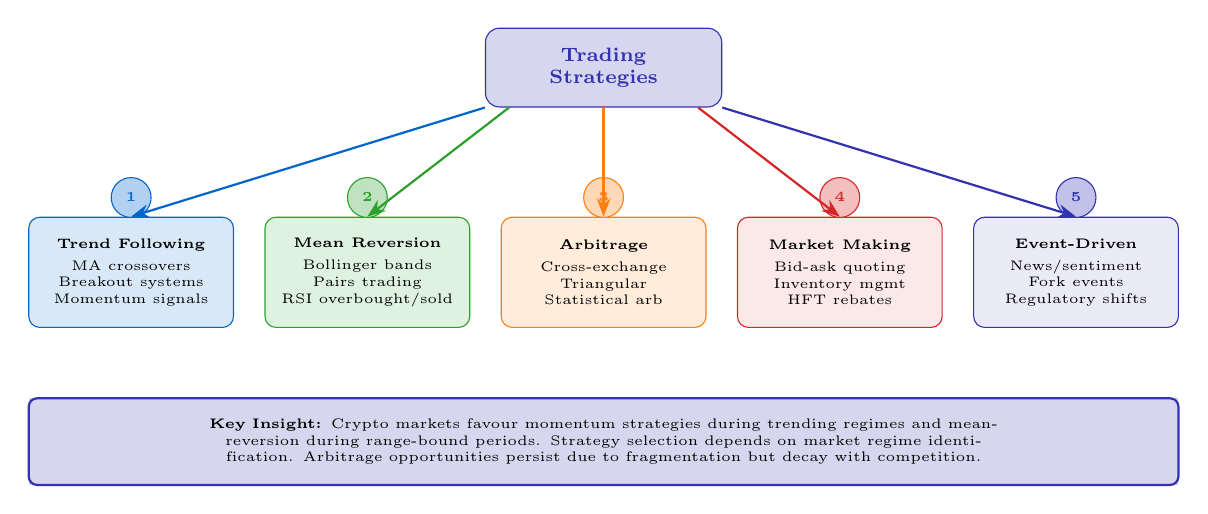
\begin{tikzpicture}
  % Root node
  \node[draw=mlpurple, fill=mlpurple!20, rounded corners=5pt, minimum width=3.0cm, minimum height=1.0cm, align=center, font=\scriptsize\bfseries, text=mlpurple] (root) at (7.5,5.8) {Trading\\Strategies};

  % Branch 1: Trend Following
  \node[draw=mlblue, fill=mlblue!15, rounded corners=4pt, minimum width=2.6cm, minimum height=1.4cm, align=center, font=\tiny] (b1) at (1.5,3.2) {\textbf{Trend Following}\\[2pt]MA crossovers\\Breakout systems\\Momentum signals};
  \node[circle, draw=mlblue, fill=mlblue!30, minimum size=0.45cm, font=\tiny\bfseries, text=mlblue] at (1.5,4.15) {1};

  % Branch 2: Mean Reversion
  \node[draw=mlgreen, fill=mlgreen!15, rounded corners=4pt, minimum width=2.6cm, minimum height=1.4cm, align=center, font=\tiny] (b2) at (4.5,3.2) {\textbf{Mean Reversion}\\[2pt]Bollinger bands\\Pairs trading\\RSI overbought/sold};
  \node[circle, draw=mlgreen, fill=mlgreen!30, minimum size=0.45cm, font=\tiny\bfseries, text=mlgreen] at (4.5,4.15) {2};

  % Branch 3: Arbitrage
  \node[draw=mlorange, fill=mlorange!15, rounded corners=4pt, minimum width=2.6cm, minimum height=1.4cm, align=center, font=\tiny] (b3) at (7.5,3.2) {\textbf{Arbitrage}\\[2pt]Cross-exchange\\Triangular\\Statistical arb};
  \node[circle, draw=mlorange, fill=mlorange!30, minimum size=0.45cm, font=\tiny\bfseries, text=mlorange] at (7.5,4.15) {3};

  % Branch 4: Market Making
  \node[draw=mlred, fill=mlred!10, rounded corners=4pt, minimum width=2.6cm, minimum height=1.4cm, align=center, font=\tiny] (b4) at (10.5,3.2) {\textbf{Market Making}\\[2pt]Bid-ask quoting\\Inventory mgmt\\HFT rebates};
  \node[circle, draw=mlred, fill=mlred!30, minimum size=0.45cm, font=\tiny\bfseries, text=mlred] at (10.5,4.15) {4};

  % Branch 5: Event-Driven
  \node[draw=mlpurple, fill=mlpurple!10, rounded corners=4pt, minimum width=2.6cm, minimum height=1.4cm, align=center, font=\tiny] (b5) at (13.5,3.2) {\textbf{Event-Driven}\\[2pt]News/sentiment\\Fork events\\Regulatory shifts};
  \node[circle, draw=mlpurple, fill=mlpurple!30, minimum size=0.45cm, font=\tiny\bfseries, text=mlpurple] at (13.5,4.15) {5};

  % Arrows from root to branches
  \draw[-{Stealth}, thick, mlblue] (root.south west) -- (b1.north);
  \draw[-{Stealth}, thick, mlgreen] (root.south) +(-1.2,0) -- (b2.north);
  \draw[-{Stealth}, thick, mlorange] (root.south) -- (b3.north);
  \draw[-{Stealth}, thick, mlred] (root.south) +(1.2,0) -- (b4.north);
  \draw[-{Stealth}, thick, mlpurple] (root.south east) -- (b5.north);

  % Bottom annotation bar
  \fill[mllavender4] (0.2,0.5) rectangle (14.8,1.6);
  \draw[mlpurple, thick, rounded corners=3pt] (0.2,0.5) rectangle (14.8,1.6);
  \node[font=\tiny, align=center, text width=14cm] at (7.5,1.05) {\textbf{Key Insight:} Crypto markets favour momentum strategies during trending regimes and mean-reversion during range-bound periods. Strategy selection depends on market regime identification. Arbitrage opportunities persist due to fragmentation but decay with competition.};
\end{tikzpicture}
\bottomnote{5 strategy families: trend following, mean reversion, arbitrage, market making, event-driven | Regime-dependent selection is critical}
\end{frame}

% Frame 17: Momentum & Trend Following
\begin{frame}{Momentum \& Trend Following}
\begin{columns}[T]
\column{0.42\textwidth}
\begin{block}{Core Concept}
\begin{itemize}\setlength{\itemsep}{2pt}
  \item \textbf{Premise:} Assets that have risen tend to continue rising (and vice versa)
  \item \textbf{Time horizon:} Days to months
  \item \textbf{Signal:} Fast MA crosses above slow MA $\Rightarrow$ bullish
  \item \textbf{Crypto edge:} Strong momentum effects due to retail-driven hype cycles and low institutional mean-reversion
\end{itemize}
\end{block}
\vspace{1mm}
\begin{alertblock}{Golden Cross / Death Cross}
\scriptsize \textbf{Golden Cross:} 50-day MA crosses above 200-day MA --- historically bullish signal. \textbf{Death Cross:} 50-day MA crosses below 200-day MA --- bearish signal. Crypto traders use shorter windows (20/50) due to faster cycles.
\end{alertblock}
\column{0.58\textwidth}
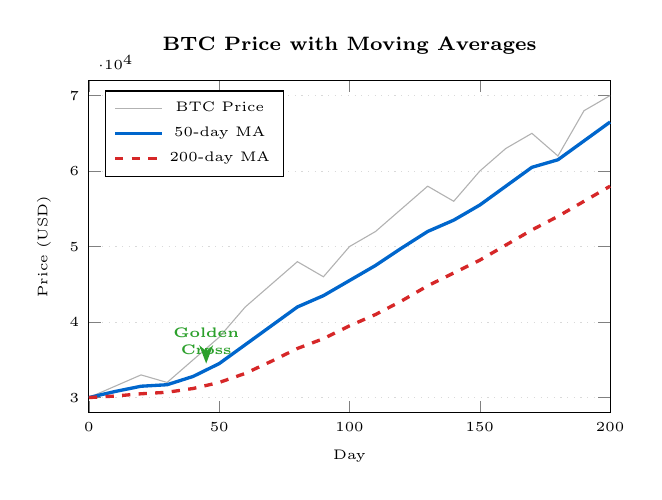
\begin{tikzpicture}
\begin{axis}[
  width=8.2cm, height=5.8cm,
  title={\scriptsize\bfseries BTC Price with Moving Averages},
  xlabel={\tiny Day},
  ylabel={\tiny Price (USD)},
  xmin=0, xmax=200,
  ymin=28000, ymax=72000,
  x tick label style={font=\tiny},
  y tick label style={font=\tiny},
  ymajorgrids=true,
  grid style={dotted, mlgray!30},
  legend style={font=\tiny, at={(0.03,0.97)}, anchor=north west},
  every axis plot/.append style={thick},
  clip=false
]
% BTC price (simulated trend with noise)
\addplot[mlgray!60, thin] coordinates {
  (0,30000) (10,31500) (20,33000) (30,32000) (40,35000)
  (50,38000) (60,42000) (70,45000) (80,48000) (90,46000)
  (100,50000) (110,52000) (120,55000) (130,58000) (140,56000)
  (150,60000) (160,63000) (170,65000) (180,62000) (190,68000)
  (200,70000)
};
\addlegendentry{BTC Price}
% 50-day MA (fast)
\addplot[mlblue, very thick] coordinates {
  (0,30000) (10,30800) (20,31500) (30,31700) (40,32800)
  (50,34500) (60,37000) (70,39500) (80,42000) (90,43500)
  (100,45500) (110,47500) (120,49800) (130,52000) (140,53500)
  (150,55500) (160,58000) (170,60500) (180,61500) (190,64000)
  (200,66500)
};
\addlegendentry{50-day MA}
% 200-day MA (slow)
\addplot[mlred, very thick, dashed] coordinates {
  (0,30000) (10,30200) (20,30500) (30,30700) (40,31200)
  (50,32000) (60,33200) (70,34800) (80,36500) (90,37800)
  (100,39500) (110,41000) (120,42800) (130,44800) (140,46500)
  (150,48200) (160,50200) (170,52200) (180,54000) (190,56000)
  (200,58000)
};
\addlegendentry{200-day MA}
% Golden cross annotation
\node[font=\tiny\bfseries, text=mlgreen, align=center] at (axis cs:45,37500) {Golden\\Cross};
\draw[-{Stealth}, thick, mlgreen] (axis cs:45,36500) -- (axis cs:45,34500);
\end{axis}
\end{tikzpicture}
\end{columns}
\bottomnote{Momentum: ``trend is your friend'' | Golden cross (50MA $>$ 200MA) = bullish | Death cross = bearish | Crypto momentum amplified by retail-driven cycles}
\end{frame}

% Frame 18: Moving Average Crossover
\begin{frame}{Moving Average Crossover}
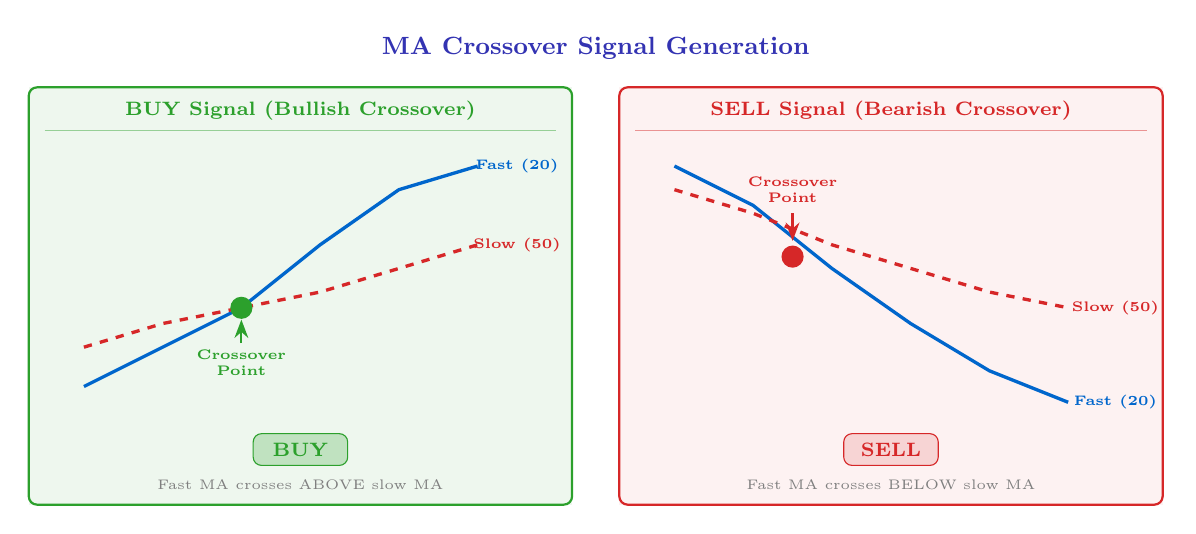
\begin{tikzpicture}
  % Title
  \node[font=\small\bfseries, text=mlpurple] at (7.5,6.3) {MA Crossover Signal Generation};

  % Left panel: BUY signal
  \fill[mlgreen!8] (0.3,0.5) rectangle (7.2,5.8);
  \draw[mlgreen, thick, rounded corners=3pt] (0.3,0.5) rectangle (7.2,5.8);
  \node[font=\scriptsize\bfseries, text=mlgreen] at (3.75,5.5) {BUY Signal (Bullish Crossover)};
  \draw[mlgreen!50] (0.5,5.25) -- (7.0,5.25);

  % Fast MA line going up, crossing slow MA
  \draw[mlblue, very thick] (1.0,2.0) -- (2.0,2.5) -- (3.0,3.0) -- (4.0,3.8) -- (5.0,4.5) -- (6.0,4.8);
  \node[font=\tiny\bfseries, text=mlblue] at (6.5,4.8) {Fast (20)};

  \draw[mlred, very thick, dashed] (1.0,2.5) -- (2.0,2.8) -- (3.0,3.0) -- (4.0,3.2) -- (5.0,3.5) -- (6.0,3.8);
  \node[font=\tiny\bfseries, text=mlred] at (6.5,3.8) {Slow (50)};

  % Crossover point
  \fill[mlgreen] (3.0,3.0) circle (4pt);
  \node[font=\tiny\bfseries, text=mlgreen, align=center] at (3.0,2.3) {Crossover\\Point};
  \draw[-{Stealth}, thick, mlgreen] (3.0,2.55) -- (3.0,2.85);

  % BUY arrow
  \node[draw=mlgreen, fill=mlgreen!30, rounded corners=3pt, font=\scriptsize\bfseries, text=mlgreen, minimum width=1.2cm] at (3.75,1.2) {BUY};
  \node[font=\tiny, text=mlgray, align=center] at (3.75,0.75) {Fast MA crosses ABOVE slow MA};

  % Right panel: SELL signal
  \fill[mlred!6] (7.8,0.5) rectangle (14.7,5.8);
  \draw[mlred, thick, rounded corners=3pt] (7.8,0.5) rectangle (14.7,5.8);
  \node[font=\scriptsize\bfseries, text=mlred] at (11.25,5.5) {SELL Signal (Bearish Crossover)};
  \draw[mlred!50] (8.0,5.25) -- (14.5,5.25);

  % Fast MA line going down, crossing slow MA
  \draw[mlblue, very thick] (8.5,4.8) -- (9.5,4.3) -- (10.5,3.5) -- (11.5,2.8) -- (12.5,2.2) -- (13.5,1.8);
  \node[font=\tiny\bfseries, text=mlblue] at (14.1,1.8) {Fast (20)};

  \draw[mlred, very thick, dashed] (8.5,4.5) -- (9.5,4.2) -- (10.5,3.8) -- (11.5,3.5) -- (12.5,3.2) -- (13.5,3.0);
  \node[font=\tiny\bfseries, text=mlred] at (14.1,3.0) {Slow (50)};

  % Crossover point
  \fill[mlred] (10.0,3.65) circle (4pt);
  \node[font=\tiny\bfseries, text=mlred, align=center] at (10.0,4.5) {Crossover\\Point};
  \draw[-{Stealth}, thick, mlred] (10.0,4.2) -- (10.0,3.85);

  % SELL arrow
  \node[draw=mlred, fill=mlred!20, rounded corners=3pt, font=\scriptsize\bfseries, text=mlred, minimum width=1.2cm] at (11.25,1.2) {SELL};
  \node[font=\tiny, text=mlgray, align=center] at (11.25,0.75) {Fast MA crosses BELOW slow MA};
\end{tikzpicture}
\bottomnote{MA crossover: fast (20-day) vs slow (50-day) | Fast above slow = BUY | Fast below slow = SELL | Sensitive to parameter choice and whipsaws}
\end{frame}

% Frame 19: Bollinger Bands & Mean Reversion
\begin{frame}{Bollinger Bands \& Mean Reversion}
\begin{columns}[T]
\column{0.42\textwidth}
\begin{block}{Bollinger Bands Definition}
\begin{itemize}\setlength{\itemsep}{2pt}
  \item \textbf{Middle band:} $\text{SMA}(n)$ --- typically $n=20$
  \item \textbf{Upper band:} $\text{SMA} + k\sigma$
  \item \textbf{Lower band:} $\text{SMA} - k\sigma$
  \item Standard: $k=2$ captures $\approx$95\% of price action
\end{itemize}
\end{block}
\vspace{1mm}
\begin{block}{Mean-Reversion Logic}
\begin{itemize}\setlength{\itemsep}{2pt}
  \item Price touches \textbf{upper band} $\Rightarrow$ overbought $\Rightarrow$ potential sell
  \item Price touches \textbf{lower band} $\Rightarrow$ oversold $\Rightarrow$ potential buy
  \item \textbf{Squeeze:} Bands narrow $\Rightarrow$ low volatility $\Rightarrow$ breakout imminent
  \item Works best in \textbf{range-bound} markets; fails during strong trends
\end{itemize}
\end{block}
\column{0.58\textwidth}
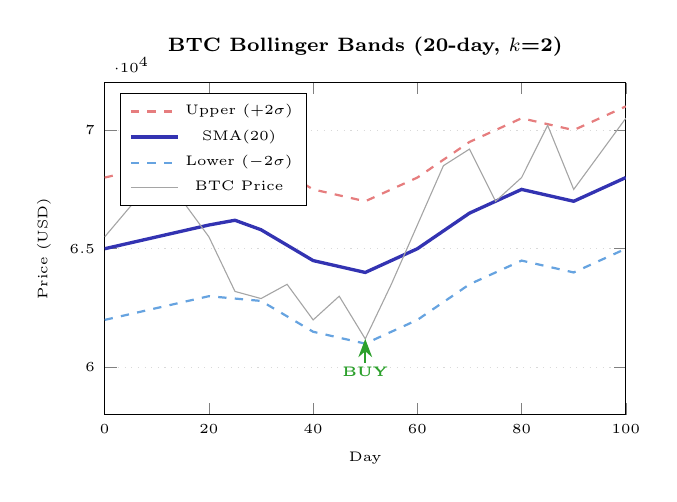
\begin{tikzpicture}
\begin{axis}[
  width=8.2cm, height=5.8cm,
  title={\scriptsize\bfseries BTC Bollinger Bands (20-day, $k$=2)},
  xlabel={\tiny Day},
  ylabel={\tiny Price (USD)},
  xmin=0, xmax=100,
  ymin=58000, ymax=72000,
  x tick label style={font=\tiny},
  y tick label style={font=\tiny},
  ymajorgrids=true,
  grid style={dotted, mlgray!30},
  legend style={font=\tiny, at={(0.03,0.97)}, anchor=north west},
  every axis plot/.append style={thick}
]
% Upper band
\addplot[mlred!60, thick, dashed] coordinates {
  (0,68000) (10,68500) (20,69000) (25,69500) (30,68800)
  (40,67500) (50,67000) (60,68000) (70,69500) (80,70500)
  (90,70000) (100,71000)
};
\addlegendentry{Upper ($+2\sigma$)}
% SMA (middle)
\addplot[mlpurple, very thick] coordinates {
  (0,65000) (10,65500) (20,66000) (25,66200) (30,65800)
  (40,64500) (50,64000) (60,65000) (70,66500) (80,67500)
  (90,67000) (100,68000)
};
\addlegendentry{SMA(20)}
% Lower band
\addplot[mlblue!60, thick, dashed] coordinates {
  (0,62000) (10,62500) (20,63000) (25,62900) (30,62800)
  (40,61500) (50,61000) (60,62000) (70,63500) (80,64500)
  (90,64000) (100,65000)
};
\addlegendentry{Lower ($-2\sigma$)}
% BTC price bouncing within bands
\addplot[mlgray!70, thin] coordinates {
  (0,65500) (5,66800) (10,68200) (15,67000) (20,65500)
  (25,63200) (30,62900) (35,63500) (40,62000) (45,63000)
  (50,61200) (55,63500) (60,66000) (65,68500) (70,69200)
  (75,67000) (80,68000) (85,70200) (90,67500) (95,69000)
  (100,70500)
};
\addlegendentry{BTC Price}
% Buy signal annotation
\node[font=\tiny\bfseries, text=mlgreen] at (axis cs:50,59800) {BUY};
\draw[-{Stealth}, thick, mlgreen] (axis cs:50,60200) -- (axis cs:50,61200);
% Sell signal annotation
\node[font=\tiny\bfseries, text=mlred] at (axis cs:10,70200) {SELL};
\draw[-{Stealth}, thick, mlred] (axis cs:10,69800) -- (axis cs:10,68700);
\end{axis}
\end{tikzpicture}
\end{columns}
\bottomnote{Bollinger Bands: SMA $\pm$ $k\sigma$ | Touch upper = overbought (sell), touch lower = oversold (buy) | Squeeze signals volatility breakout | Best in range-bound markets}
\end{frame}

% Frame 20: Strategy Implementation [FRAGILE] -- CODE FRAME 2
\begin{frame}[fragile]{Strategy Implementation}
\begin{columns}[T]
\column{0.50\textwidth}
\begin{lstlisting}[language=Python, caption={Moving Average Crossover Strategy}]
# Moving Average Crossover Strategy
import numpy as np

def ma_crossover(prices, fast=20,
                 slow=50):
    fast_ma = sma(prices, fast)
    slow_ma = sma(prices, slow)
    signals = []

    for i in range(1, len(prices)):
        if (fast_ma[i] > slow_ma[i] and
            fast_ma[i-1] <= slow_ma[i-1]):
            signals.append(("BUY", i))
        elif (fast_ma[i] < slow_ma[i] and
              fast_ma[i-1] >= slow_ma[i-1]):
            signals.append(("SELL", i))
    return signals
\end{lstlisting}
\vspace{1mm}
\begin{alertblock}{Key Principle}
\scriptsize Crossover strategies detect \textbf{regime changes}: the moment short-term momentum diverges from the long-term trend. Signal quality depends heavily on parameter selection.
\end{alertblock}
\column{0.50\textwidth}
\begin{block}{Signal Generation Logic}
\begin{itemize}\setlength{\itemsep}{2pt}
  \item \textbf{BUY:} Fast MA crosses above slow MA at time $t$ (bullish momentum shift)
  \item \textbf{SELL:} Fast MA crosses below slow MA at time $t$ (bearish momentum shift)
  \item \textbf{Detection:} Compare current and previous bar to identify exact crossover point
\end{itemize}
\end{block}
\vspace{2mm}
\begin{block}{Parameter Sensitivity}
\begin{itemize}\setlength{\itemsep}{2pt}
  \item \textbf{Fast window (20):} Shorter = more signals but more whipsaws; longer = fewer but later signals
  \item \textbf{Slow window (50):} Anchors the trend baseline; 50/200 is traditional, 20/50 common in crypto
  \item \textbf{Overfitting risk:} Optimising parameters on historical data often fails out-of-sample
  \item \textbf{Mitigation:} Walk-forward optimisation, cross-validation across market regimes
\end{itemize}
\end{block}
\end{columns}
\bottomnote{MA crossover implementation: detect fast/slow MA crossings | Parameters: fast=20, slow=50 | Risk: overfitting to historical data | Use walk-forward validation}
\end{frame}

% Frame 21: Cross-Exchange Arbitrage
\begin{frame}{Cross-Exchange Arbitrage}
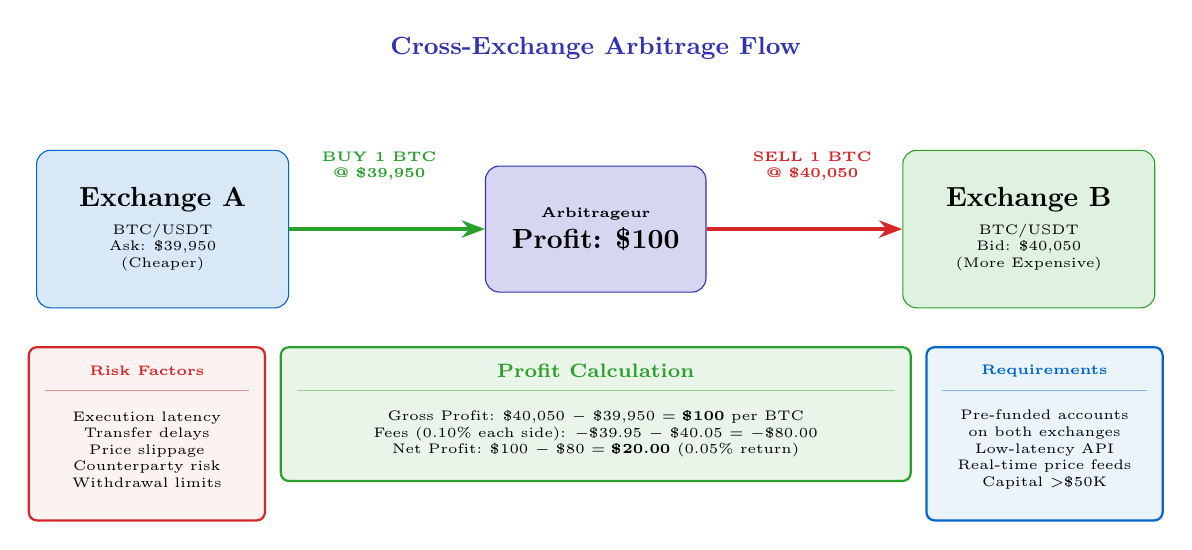
\begin{tikzpicture}
  % Title
  \node[font=\small\bfseries, text=mlpurple] at (7.5,6.3) {Cross-Exchange Arbitrage Flow};

  % Exchange A
  \node[draw=mlblue, fill=mlblue!15, rounded corners=5pt, minimum width=3.2cm, minimum height=2.0cm, align=center, font=\tiny] (exA) at (2.0,4.0) {\textbf{\normalsize Exchange A}\\[4pt]BTC/USDT\\Ask: \$39,950\\(Cheaper)};

  % Exchange B
  \node[draw=mlgreen, fill=mlgreen!15, rounded corners=5pt, minimum width=3.2cm, minimum height=2.0cm, align=center, font=\tiny] (exB) at (13.0,4.0) {\textbf{\normalsize Exchange B}\\[4pt]BTC/USDT\\Bid: \$40,050\\(More Expensive)};

  % Arbitrageur
  \node[draw=mlpurple, fill=mlpurple!20, rounded corners=5pt, minimum width=2.8cm, minimum height=1.6cm, align=center, font=\tiny\bfseries] (arb) at (7.5,4.0) {Arbitrageur\\[2pt]\normalsize Profit: \$100};

  % Buy arrow
  \draw[-{Stealth}, very thick, mlgreen] (exA.east) -- (arb.west);
  \node[font=\tiny\bfseries, text=mlgreen, align=center] at (4.75,4.8) {BUY 1 BTC\\@ \$39,950};

  % Sell arrow
  \draw[-{Stealth}, very thick, mlred] (arb.east) -- (exB.west);
  \node[font=\tiny\bfseries, text=mlred, align=center] at (10.25,4.8) {SELL 1 BTC\\@ \$40,050};

  % Profit calculation
  \fill[mlgreen!10] (3.5,0.8) rectangle (11.5,2.5);
  \draw[mlgreen, thick, rounded corners=3pt] (3.5,0.8) rectangle (11.5,2.5);
  \node[font=\scriptsize\bfseries, text=mlgreen] at (7.5,2.2) {Profit Calculation};
  \draw[mlgreen!50] (3.7,1.95) -- (11.3,1.95);
  \node[font=\tiny, align=center] at (7.5,1.4) {Gross Profit: \$40,050 $-$ \$39,950 = \textbf{\$100} per BTC\\Fees (0.10\% each side): $-$\$39.95 $-$ \$40.05 = $-$\$80.00\\Net Profit: \$100 $-$ \$80 = \textbf{\$20.00} (0.05\% return)};

  % Risk factors
  \fill[mlred!6] (0.3,0.3) rectangle (3.3,2.5);
  \draw[mlred, thick, rounded corners=3pt] (0.3,0.3) rectangle (3.3,2.5);
  \node[font=\tiny\bfseries, text=mlred] at (1.8,2.2) {Risk Factors};
  \draw[mlred!50] (0.5,1.95) -- (3.1,1.95);
  \node[font=\tiny, align=center, text width=2.6cm] at (1.8,1.2) {Execution latency\\Transfer delays\\Price slippage\\Counterparty risk\\Withdrawal limits};

  % Requirements
  \fill[mlblue!8] (11.7,0.3) rectangle (14.7,2.5);
  \draw[mlblue, thick, rounded corners=3pt] (11.7,0.3) rectangle (14.7,2.5);
  \node[font=\tiny\bfseries, text=mlblue] at (13.2,2.2) {Requirements};
  \draw[mlblue!50] (11.9,1.95) -- (14.5,1.95);
  \node[font=\tiny, align=center, text width=2.6cm] at (13.2,1.2) {Pre-funded accounts\\on both exchanges\\Low-latency API\\Real-time price feeds\\Capital $>$\$50K};
\end{tikzpicture}
\bottomnote{Cross-exchange arb: buy low on Exchange A, sell high on Exchange B simultaneously | Net profit after fees: $\sim$0.05\% | Requires pre-funded accounts and fast execution}
\end{frame}

% Frame 22: Triangular Arbitrage
\begin{frame}{Triangular Arbitrage}
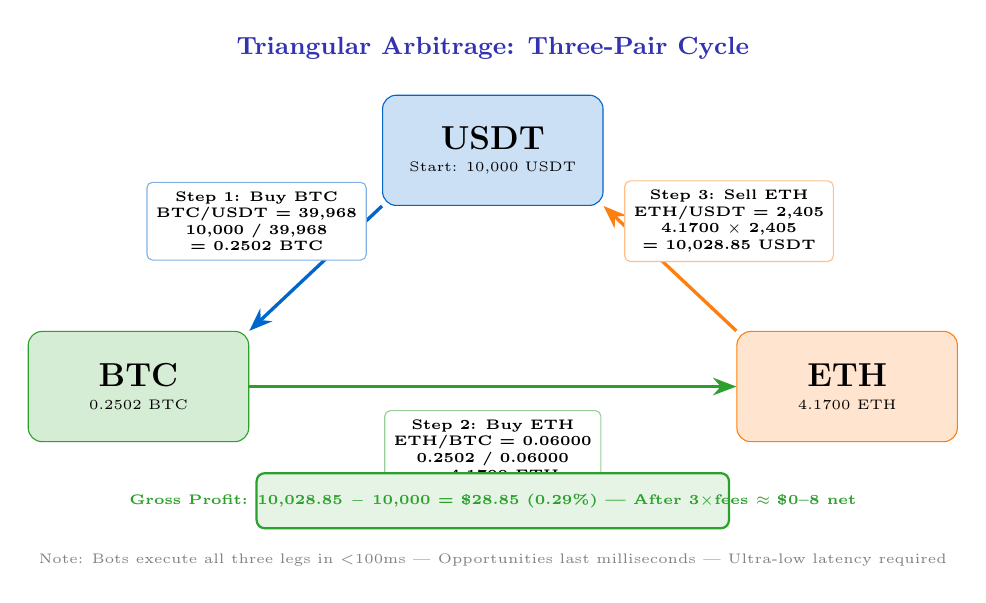
\begin{tikzpicture}
  % Title
  \node[font=\small\bfseries, text=mlpurple] at (7.5,6.3) {Triangular Arbitrage: Three-Pair Cycle};

  % Triangle vertices
  \node[draw=mlblue, fill=mlblue!20, rounded corners=5pt, minimum width=2.8cm, minimum height=1.4cm, align=center, font=\tiny] (usdt) at (7.5,5.0) {\textbf{\large USDT}\\[2pt]Start: 10{,}000 USDT};

  \node[draw=mlgreen, fill=mlgreen!20, rounded corners=5pt, minimum width=2.8cm, minimum height=1.4cm, align=center, font=\tiny] (btc) at (3.0,2.0) {\textbf{\large BTC}\\[2pt]0.2502 BTC};

  \node[draw=mlorange, fill=mlorange!20, rounded corners=5pt, minimum width=2.8cm, minimum height=1.4cm, align=center, font=\tiny] (eth) at (12.0,2.0) {\textbf{\large ETH}\\[2pt]4.1700 ETH};

  % Step 1: USDT -> BTC
  \draw[-{Stealth}, very thick, mlblue] (usdt.south west) -- (btc.north east);
  \node[draw=mlblue!50, fill=white, rounded corners=2pt, font=\tiny\bfseries, align=center] at (4.5,4.1) {Step 1: Buy BTC\\BTC/USDT = 39{,}968\\10{,}000 / 39{,}968\\= 0.2502 BTC};

  % Step 2: BTC -> ETH
  \draw[-{Stealth}, very thick, mlgreen] (btc.east) -- (eth.west);
  \node[draw=mlgreen!50, fill=white, rounded corners=2pt, font=\tiny\bfseries, align=center] at (7.5,1.2) {Step 2: Buy ETH\\ETH/BTC = 0.06000\\0.2502 / 0.06000\\= 4.1700 ETH};

  % Step 3: ETH -> USDT
  \draw[-{Stealth}, very thick, mlorange] (eth.north west) -- (usdt.south east);
  \node[draw=mlorange!50, fill=white, rounded corners=2pt, font=\tiny\bfseries, align=center] at (10.5,4.1) {Step 3: Sell ETH\\ETH/USDT = 2{,}405\\4.1700 $\times$ 2{,}405\\= 10{,}028.85 USDT};

  % Profit box
  \fill[mlgreen!12] (4.5,0.2) rectangle (10.5,0.9);
  \draw[mlgreen, thick, rounded corners=3pt] (4.5,0.2) rectangle (10.5,0.9);
  \node[font=\tiny\bfseries, text=mlgreen, align=center] at (7.5,0.55) {Gross Profit: 10{,}028.85 $-$ 10{,}000 = \$28.85 (0.29\%) | After 3$\times$fees $\approx$ \$0--8 net};

  % Note
  \node[font=\tiny, text=mlgray, align=center] at (7.5,-0.2) {Note: Bots execute all three legs in $<$100ms | Opportunities last milliseconds | Ultra-low latency required};
\end{tikzpicture}
\bottomnote{Triangular arb: USDT $\to$ BTC $\to$ ETH $\to$ USDT cycle exploiting cross-pair mispricing | Gross 0.29\% but fees erode profit | Bot-only, $<$100ms execution}
\end{frame}

% Frame 23: Statistical Arbitrage (Pairs Trading)
\begin{frame}{Statistical Arbitrage (Pairs Trading)}
\begin{columns}[T]
\column{0.42\textwidth}
\begin{block}{Pairs Trading Concept}
\begin{itemize}\setlength{\itemsep}{2pt}
  \item \textbf{Idea:} Two correlated assets (e.g., BTC and ETH) tend to move together
  \item \textbf{Spread:} $S_t = P_t^{\text{BTC}} - \beta \cdot P_t^{\text{ETH}}$
  \item \textbf{Signal:} When spread deviates $>2\sigma$ from mean, bet on convergence
  \item \textbf{Entry:} Long the underperformer, short the outperformer
  \item \textbf{Exit:} Spread returns to mean (or stop-loss at $3\sigma$)
\end{itemize}
\end{block}
\vspace{1mm}
\begin{alertblock}{Crypto Pairs}
\scriptsize Popular pairs: BTC/ETH, SOL/AVAX, stablecoin depegs (USDT/USDC). Crypto pairs show higher correlation during drawdowns (correlation breakdown risk).
\end{alertblock}
\column{0.58\textwidth}
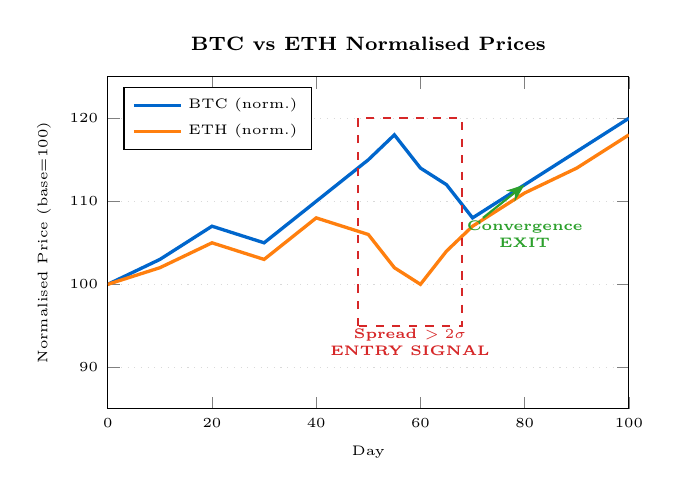
\begin{tikzpicture}
\begin{axis}[
  width=8.2cm, height=5.8cm,
  title={\scriptsize\bfseries BTC vs ETH Normalised Prices},
  xlabel={\tiny Day},
  ylabel={\tiny Normalised Price (base=100)},
  xmin=0, xmax=100,
  ymin=85, ymax=125,
  x tick label style={font=\tiny},
  y tick label style={font=\tiny},
  ymajorgrids=true,
  grid style={dotted, mlgray!30},
  legend style={font=\tiny, at={(0.03,0.97)}, anchor=north west},
  every axis plot/.append style={thick}
]
% BTC normalised
\addplot[mlblue, very thick] coordinates {
  (0,100) (10,103) (20,107) (30,105) (40,110)
  (50,115) (55,118) (60,114) (65,112) (70,108)
  (80,112) (90,116) (100,120)
};
\addlegendentry{BTC (norm.)}
% ETH normalised -- diverges then converges
\addplot[mlorange, very thick] coordinates {
  (0,100) (10,102) (20,105) (30,103) (40,108)
  (50,106) (55,102) (60,100) (65,104) (70,107)
  (80,111) (90,114) (100,118)
};
\addlegendentry{ETH (norm.)}
% Divergence zone
\draw[mlred, thick, dashed] (axis cs:48,95) rectangle (axis cs:68,120);
\node[font=\tiny\bfseries, text=mlred, align=center] at (axis cs:58,93) {Spread $> 2\sigma$\\ENTRY SIGNAL};
% Convergence annotation
\draw[-{Stealth}, thick, mlgreen] (axis cs:72,108) -- (axis cs:80,112);
\node[font=\tiny\bfseries, text=mlgreen, align=center] at (axis cs:80,106) {Convergence\\EXIT};
\end{axis}
\end{tikzpicture}
\end{columns}
\bottomnote{Stat arb: long underperformer + short outperformer when spread $> 2\sigma$ | Exit on mean reversion | Risk: regime change breaks correlation}
\end{frame}

% Frame 24: Technical Indicators Overview
\begin{frame}{Technical Indicators Overview}
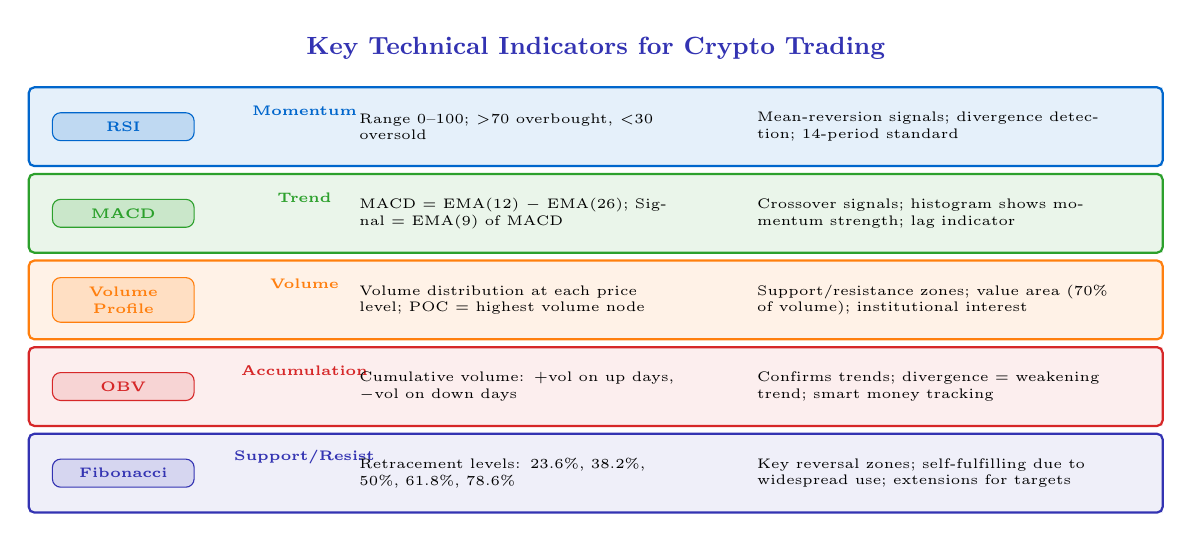
\begin{tikzpicture}
  % Title
  \node[font=\small\bfseries, text=mlpurple] at (7.5,6.3) {Key Technical Indicators for Crypto Trading};

  % Row 1: RSI
  \fill[mlblue!10] (0.3,4.8) rectangle (14.7,5.8);
  \draw[mlblue, thick, rounded corners=2pt] (0.3,4.8) rectangle (14.7,5.8);
  \node[draw=mlblue, fill=mlblue!25, rounded corners=3pt, font=\tiny\bfseries, text=mlblue, minimum width=1.8cm, align=center] at (1.5,5.3) {RSI};
  \node[font=\tiny\bfseries, text=mlblue] at (3.8,5.5) {Momentum};
  \node[font=\tiny, text width=4.0cm] at (6.5,5.3) {Range 0--100; $>$70 overbought, $<$30 oversold};
  \node[font=\tiny, text width=4.5cm] at (11.8,5.3) {Mean-reversion signals; divergence detection; 14-period standard};

  % Row 2: MACD
  \fill[mlgreen!10] (0.3,3.7) rectangle (14.7,4.7);
  \draw[mlgreen, thick, rounded corners=2pt] (0.3,3.7) rectangle (14.7,4.7);
  \node[draw=mlgreen, fill=mlgreen!25, rounded corners=3pt, font=\tiny\bfseries, text=mlgreen, minimum width=1.8cm, align=center] at (1.5,4.2) {MACD};
  \node[font=\tiny\bfseries, text=mlgreen] at (3.8,4.4) {Trend};
  \node[font=\tiny, text width=4.0cm] at (6.5,4.2) {MACD = EMA(12) $-$ EMA(26); Signal = EMA(9) of MACD};
  \node[font=\tiny, text width=4.5cm] at (11.8,4.2) {Crossover signals; histogram shows momentum strength; lag indicator};

  % Row 3: Volume Profile
  \fill[mlorange!10] (0.3,2.6) rectangle (14.7,3.6);
  \draw[mlorange, thick, rounded corners=2pt] (0.3,2.6) rectangle (14.7,3.6);
  \node[draw=mlorange, fill=mlorange!25, rounded corners=3pt, font=\tiny\bfseries, text=mlorange, minimum width=1.8cm, align=center] at (1.5,3.1) {Volume\\Profile};
  \node[font=\tiny\bfseries, text=mlorange] at (3.8,3.3) {Volume};
  \node[font=\tiny, text width=4.0cm] at (6.5,3.1) {Volume distribution at each price level; POC = highest volume node};
  \node[font=\tiny, text width=4.5cm] at (11.8,3.1) {Support/resistance zones; value area (70\% of volume); institutional interest};

  % Row 4: OBV
  \fill[mlred!8] (0.3,1.5) rectangle (14.7,2.5);
  \draw[mlred, thick, rounded corners=2pt] (0.3,1.5) rectangle (14.7,2.5);
  \node[draw=mlred, fill=mlred!20, rounded corners=3pt, font=\tiny\bfseries, text=mlred, minimum width=1.8cm, align=center] at (1.5,2.0) {OBV};
  \node[font=\tiny\bfseries, text=mlred] at (3.8,2.2) {Accumulation};
  \node[font=\tiny, text width=4.0cm] at (6.5,2.0) {Cumulative volume: +vol on up days, $-$vol on down days};
  \node[font=\tiny, text width=4.5cm] at (11.8,2.0) {Confirms trends; divergence = weakening trend; smart money tracking};

  % Row 5: Fibonacci
  \fill[mlpurple!8] (0.3,0.4) rectangle (14.7,1.4);
  \draw[mlpurple, thick, rounded corners=2pt] (0.3,0.4) rectangle (14.7,1.4);
  \node[draw=mlpurple, fill=mlpurple!20, rounded corners=3pt, font=\tiny\bfseries, text=mlpurple, minimum width=1.8cm, align=center] at (1.5,0.9) {Fibonacci};
  \node[font=\tiny\bfseries, text=mlpurple] at (3.8,1.1) {Support/Resist};
  \node[font=\tiny, text width=4.0cm] at (6.5,0.9) {Retracement levels: 23.6\%, 38.2\%, 50\%, 61.8\%, 78.6\%};
  \node[font=\tiny, text width=4.5cm] at (11.8,0.9) {Key reversal zones; self-fulfilling due to widespread use; extensions for targets};
\end{tikzpicture}
\bottomnote{5 indicator families: RSI (momentum), MACD (trend), Volume Profile (structure), OBV (accumulation), Fibonacci (levels) | Combine multiple for confluence}
\end{frame}

% Frame 25: Backtesting Principles
\begin{frame}{Backtesting Principles}
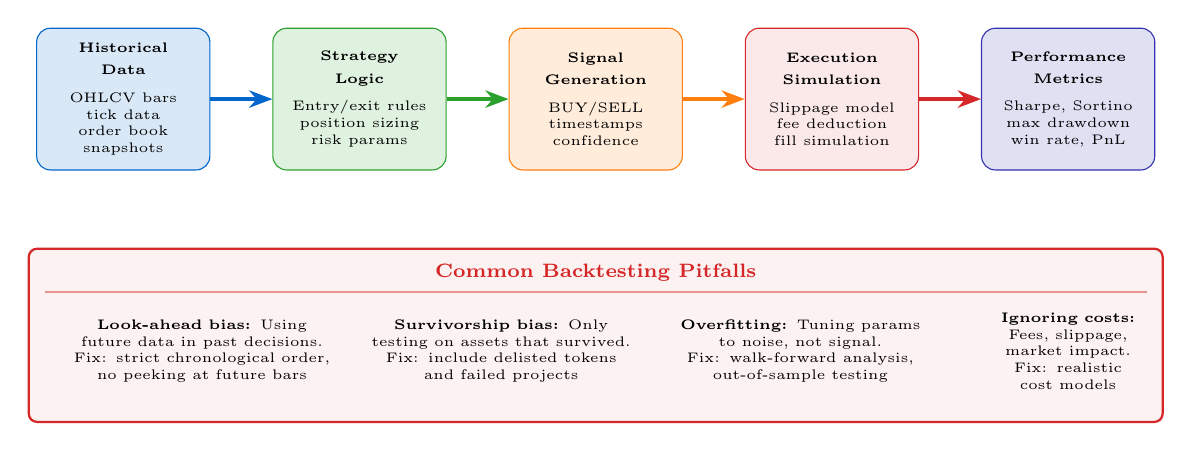
\begin{tikzpicture}
  % Pipeline: 5 stages
  \node[draw=mlblue, fill=mlblue!15, rounded corners=5pt, minimum width=2.2cm, minimum height=1.8cm, align=center, font=\tiny] (s1) at (1.5,4.5) {\textbf{Historical}\\[2pt]\textbf{Data}\\[4pt]OHLCV bars\\tick data\\order book\\snapshots};

  \node[draw=mlgreen, fill=mlgreen!15, rounded corners=5pt, minimum width=2.2cm, minimum height=1.8cm, align=center, font=\tiny] (s2) at (4.5,4.5) {\textbf{Strategy}\\[2pt]\textbf{Logic}\\[4pt]Entry/exit rules\\position sizing\\risk params};

  \node[draw=mlorange, fill=mlorange!15, rounded corners=5pt, minimum width=2.2cm, minimum height=1.8cm, align=center, font=\tiny] (s3) at (7.5,4.5) {\textbf{Signal}\\[2pt]\textbf{Generation}\\[4pt]BUY/SELL\\timestamps\\confidence};

  \node[draw=mlred, fill=mlred!10, rounded corners=5pt, minimum width=2.2cm, minimum height=1.8cm, align=center, font=\tiny] (s4) at (10.5,4.5) {\textbf{Execution}\\[2pt]\textbf{Simulation}\\[4pt]Slippage model\\fee deduction\\fill simulation};

  \node[draw=mlpurple, fill=mlpurple!15, rounded corners=5pt, minimum width=2.2cm, minimum height=1.8cm, align=center, font=\tiny] (s5) at (13.5,4.5) {\textbf{Performance}\\[2pt]\textbf{Metrics}\\[4pt]Sharpe, Sortino\\max drawdown\\win rate, PnL};

  % Arrows between stages
  \draw[-{Stealth}, very thick, mlblue] (s1.east) -- (s2.west);
  \draw[-{Stealth}, very thick, mlgreen] (s2.east) -- (s3.west);
  \draw[-{Stealth}, very thick, mlorange] (s3.east) -- (s4.west);
  \draw[-{Stealth}, very thick, mlred] (s4.east) -- (s5.west);

  % Pitfalls section
  \fill[mlred!6] (0.3,0.4) rectangle (14.7,2.6);
  \draw[mlred, thick, rounded corners=3pt] (0.3,0.4) rectangle (14.7,2.6);
  \node[font=\scriptsize\bfseries, text=mlred] at (7.5,2.3) {Common Backtesting Pitfalls};
  \draw[mlred!50] (0.5,2.05) -- (14.5,2.05);

  \node[font=\tiny, align=center, text width=3.8cm] at (2.5,1.3) {\textbf{Look-ahead bias:} Using\\future data in past decisions.\\Fix: strict chronological order,\\no peeking at future bars};

  \node[font=\tiny, align=center, text width=3.8cm] at (6.3,1.3) {\textbf{Survivorship bias:} Only\\testing on assets that survived.\\Fix: include delisted tokens\\and failed projects};

  \node[font=\tiny, align=center, text width=3.8cm] at (10.1,1.3) {\textbf{Overfitting:} Tuning params\\to noise, not signal.\\Fix: walk-forward analysis,\\out-of-sample testing};

  \node[font=\tiny, align=center, text width=2.0cm] at (13.5,1.3) {\textbf{Ignoring costs:}\\Fees, slippage,\\market impact.\\Fix: realistic\\cost models};
\end{tikzpicture}
\bottomnote{Backtesting pipeline: data $\to$ strategy $\to$ signals $\to$ execution sim $\to$ metrics | Key pitfalls: look-ahead bias, survivorship bias, overfitting, ignoring costs}
\end{frame}

% Frame 26: Section 2 Summary
\begin{frame}{Section 2 Summary}
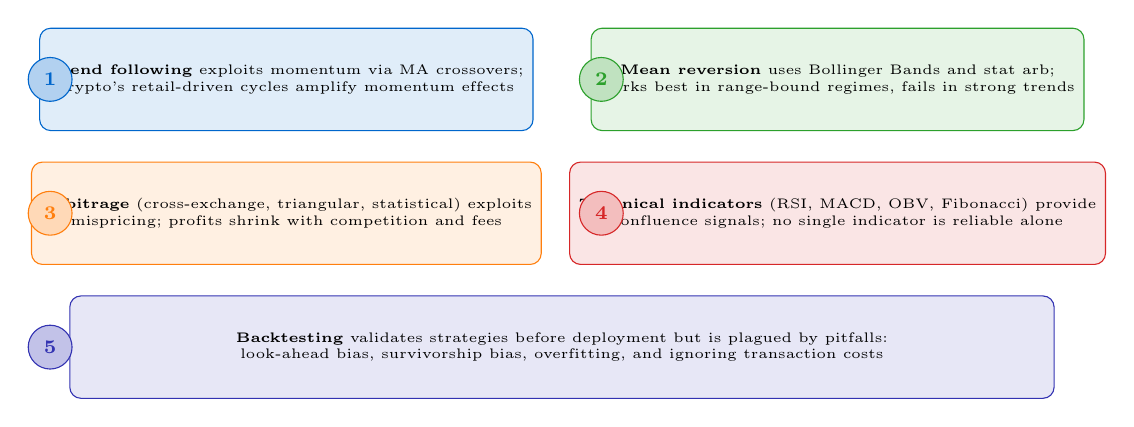
\begin{tikzpicture}
  \node[draw=mlblue, fill=mlblue!12, rounded corners=4pt, minimum width=5.5cm, minimum height=1.3cm, align=center, font=\tiny] (k1) at (4.0,5.0) {\textbf{Trend following} exploits momentum via MA crossovers;\\crypto's retail-driven cycles amplify momentum effects};
  \node[circle, draw=mlblue, fill=mlblue!30, minimum size=0.55cm, font=\scriptsize\bfseries, text=mlblue] at (1.0,5.0) {1};

  \node[draw=mlgreen, fill=mlgreen!12, rounded corners=4pt, minimum width=5.5cm, minimum height=1.3cm, align=center, font=\tiny] (k2) at (11.0,5.0) {\textbf{Mean reversion} uses Bollinger Bands and stat arb;\\works best in range-bound regimes, fails in strong trends};
  \node[circle, draw=mlgreen, fill=mlgreen!30, minimum size=0.55cm, font=\scriptsize\bfseries, text=mlgreen] at (8.0,5.0) {2};

  \node[draw=mlorange, fill=mlorange!12, rounded corners=4pt, minimum width=5.5cm, minimum height=1.3cm, align=center, font=\tiny] (k3) at (4.0,3.3) {\textbf{Arbitrage} (cross-exchange, triangular, statistical) exploits\\mispricing; profits shrink with competition and fees};
  \node[circle, draw=mlorange, fill=mlorange!30, minimum size=0.55cm, font=\scriptsize\bfseries, text=mlorange] at (1.0,3.3) {3};

  \node[draw=mlred, fill=mlred!12, rounded corners=4pt, minimum width=5.5cm, minimum height=1.3cm, align=center, font=\tiny] (k4) at (11.0,3.3) {\textbf{Technical indicators} (RSI, MACD, OBV, Fibonacci) provide\\confluence signals; no single indicator is reliable alone};
  \node[circle, draw=mlred, fill=mlred!30, minimum size=0.55cm, font=\scriptsize\bfseries, text=mlred] at (8.0,3.3) {4};

  \node[draw=mlpurple, fill=mlpurple!12, rounded corners=4pt, minimum width=12.5cm, minimum height=1.3cm, align=center, font=\tiny] (k5) at (7.5,1.6) {\textbf{Backtesting} validates strategies before deployment but is plagued by pitfalls:\\look-ahead bias, survivorship bias, overfitting, and ignoring transaction costs};
  \node[circle, draw=mlpurple, fill=mlpurple!30, minimum size=0.55cm, font=\scriptsize\bfseries, text=mlpurple] at (1.0,1.6) {5};
\end{tikzpicture}
\bottomnote{Section 2 complete | 5 key takeaways | Proceed to Section 3: Portfolio Theory \& Risk Management}
\end{frame}

%% ============================================================
%% SECTION 3: PORTFOLIO THEORY & RISK MANAGEMENT
%% ============================================================
\section{Portfolio Theory \& Risk Management}

% Frame 27: Section 3 Divider
\begin{frame}{Section 3: Portfolio Theory \& Risk Management}
\begin{beamercolorbox}[sep=12pt,center,rounded=true,shadow=true]{palette quaternary}
  {\Large\bfseries Section 3: Portfolio Theory \& Risk Management}\\[4pt]
  {\normalsize Quantitative frameworks for constructing and managing crypto portfolios}
\end{beamercolorbox}

\vspace{4mm}
\begin{columns}[T]
\column{0.55\textwidth}
\begin{block}{What You Will Learn}
\begin{itemize}\setlength{\itemsep}{2pt}
  \item Modern Portfolio Theory applied to crypto asset classes
  \item Value at Risk (VaR) and Conditional VaR (Expected Shortfall)
  \item Sharpe ratio, Sortino ratio, and risk-adjusted performance
  \item Maximum drawdown analysis and position sizing strategies
\end{itemize}
\end{block}
\column{0.45\textwidth}
\begin{block}{Frames in This Section}
\begin{itemize}\setlength{\itemsep}{2pt}
  \item Frame 28: Modern Portfolio Theory in Crypto
  \item Frame 29: Crypto Correlation Matrix
  \item Frame 30: Value at Risk (VaR)
  \item Frame 31: Expected Shortfall (CVaR)
  \item Frame 32: Sharpe Ratio \& Risk-Adjusted Returns
  \item Frame 33: Sortino Ratio \& Downside Risk
  \item Frame 34: Maximum Drawdown
  \item Frame 35: Position Sizing
  \item Frame 36: Portfolio Construction
  \item Frame 37: Risk Monitoring Dashboard
  \item Frame 38: Section 3 Summary
\end{itemize}
\end{block}
\end{columns}
\bottomnote{Section 3 of 5 | Frames 27--38 | Quantitative risk and portfolio management for digital assets}
\end{frame}

% Frame 28: Modern Portfolio Theory in Crypto
\begin{frame}{Modern Portfolio Theory in Crypto}
\begin{columns}[T]
\column{0.45\textwidth}
\begin{block}{MPT Core Concepts}
\begin{itemize}\setlength{\itemsep}{2pt}
  \item \textbf{Diversification:} Combine assets with imperfect correlations to reduce portfolio variance
  \item \textbf{Efficient frontier:} Set of portfolios offering maximum return for each risk level
  \item \textbf{Optimal portfolio:} Tangency point with the Capital Market Line (highest Sharpe ratio)
  \item \textbf{Inputs:} Expected returns $\mu_i$, volatilities $\sigma_i$, correlations $\rho_{ij}$
\end{itemize}
\end{block}
\vspace{1mm}
\begin{alertblock}{Crypto Challenge}
\scriptsize MPT assumes stationary returns and normal distributions. Crypto returns exhibit \textbf{fat tails}, \textbf{regime shifts}, and \textbf{high intra-class correlation}---limiting diversification benefits during crashes.
\end{alertblock}
\column{0.55\textwidth}
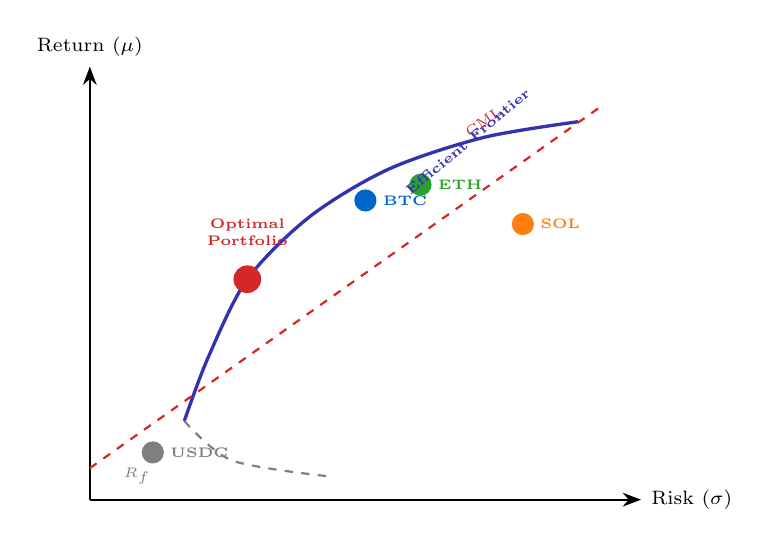
\begin{tikzpicture}
  % Axes
  \draw[-{Stealth}, thick] (0,0) -- (7.0,0) node[right, font=\scriptsize] {Risk ($\sigma$)};
  \draw[-{Stealth}, thick] (0,0) -- (0,5.5) node[above, font=\scriptsize] {Return ($\mu$)};

  % Efficient frontier curve
  \draw[mlpurple, very thick, smooth] plot coordinates {(1.2,1.0) (1.5,1.8) (2.0,2.8) (2.8,3.6) (3.8,4.2) (5.0,4.6) (6.2,4.8)};

  % Inefficient portion (dashed)
  \draw[mlgray, thick, dashed, smooth] plot coordinates {(1.2,1.0) (1.8,0.5) (3.0,0.3)};

  % Individual assets
  \fill[mlblue] (3.5,3.8) circle (4pt);
  \node[font=\tiny\bfseries, text=mlblue, right] at (3.6,3.8) {BTC};

  \fill[mlgreen] (4.2,4.0) circle (4pt);
  \node[font=\tiny\bfseries, text=mlgreen, right] at (4.3,4.0) {ETH};

  \fill[mlorange] (5.5,3.5) circle (4pt);
  \node[font=\tiny\bfseries, text=mlorange, right] at (5.6,3.5) {SOL};

  \fill[mlgray] (0.8,0.6) circle (4pt);
  \node[font=\tiny\bfseries, text=mlgray, right] at (0.9,0.6) {USDC};

  % Optimal portfolio (tangency)
  \fill[mlred] (2.0,2.8) circle (5pt);
  \node[font=\tiny\bfseries, text=mlred, align=center] at (2.0,3.4) {Optimal\\Portfolio};

  % Capital Market Line
  \draw[mlred, thick, dashed] (0,0.4) -- (6.5,5.0);
  \node[font=\tiny, text=mlred, rotate=35] at (5.0,4.8) {CML};

  % Risk-free rate
  \node[font=\tiny, text=mlgray] at (0.6,0.3) {$R_f$};

  % Label
  \node[font=\tiny\bfseries, text=mlpurple, rotate=40] at (4.8,4.55) {Efficient Frontier};
\end{tikzpicture}
\end{columns}
\bottomnote{MPT: Markowitz (1952) | Efficient frontier maximises return per unit risk | Crypto's high correlation limits diversification, especially in drawdowns}
\end{frame}

% Frame 29: Crypto Correlation Matrix
\begin{frame}{Crypto Correlation Matrix}
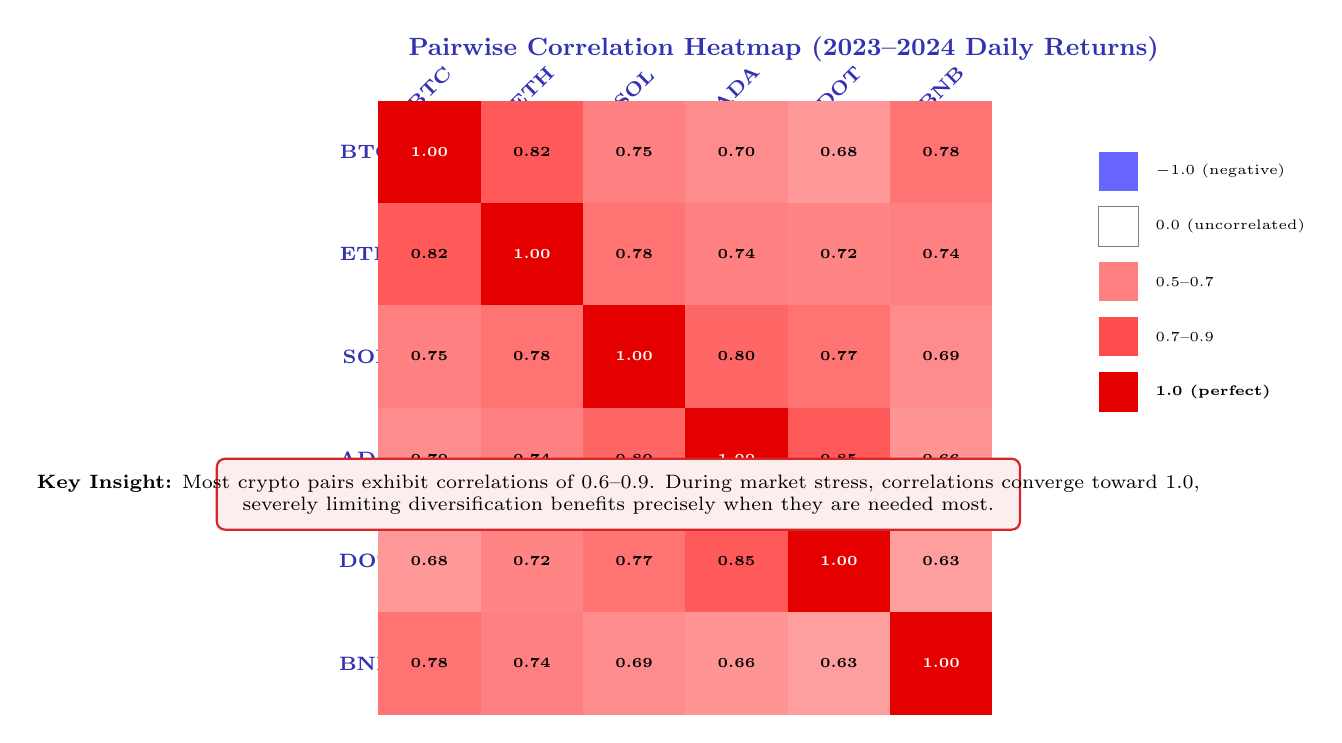
\begin{tikzpicture}
  % Title
  \node[font=\small\bfseries, text=mlpurple] at (7.5,6.3) {Pairwise Correlation Heatmap (2023--2024 Daily Returns)};

  % Assets
  \def\assets{{"BTC","ETH","SOL","ADA","DOT","BNB"}}

  % Grid parameters
  \def\cellsize{1.3}
  \def\startx{3.0}
  \def\starty{5.0}

  % Row/column labels
  \node[font=\scriptsize\bfseries, text=mlpurple] at (\startx - 0.8, \starty - 0*\cellsize) {BTC};
  \node[font=\scriptsize\bfseries, text=mlpurple] at (\startx - 0.8, \starty - 1*\cellsize) {ETH};
  \node[font=\scriptsize\bfseries, text=mlpurple] at (\startx - 0.8, \starty - 2*\cellsize) {SOL};
  \node[font=\scriptsize\bfseries, text=mlpurple] at (\startx - 0.8, \starty - 3*\cellsize) {ADA};
  \node[font=\scriptsize\bfseries, text=mlpurple] at (\startx - 0.8, \starty - 4*\cellsize) {DOT};
  \node[font=\scriptsize\bfseries, text=mlpurple] at (\startx - 0.8, \starty - 5*\cellsize) {BNB};

  \node[font=\scriptsize\bfseries, text=mlpurple, rotate=45] at (\startx + 0*\cellsize, \starty + 0.8) {BTC};
  \node[font=\scriptsize\bfseries, text=mlpurple, rotate=45] at (\startx + 1*\cellsize, \starty + 0.8) {ETH};
  \node[font=\scriptsize\bfseries, text=mlpurple, rotate=45] at (\startx + 2*\cellsize, \starty + 0.8) {SOL};
  \node[font=\scriptsize\bfseries, text=mlpurple, rotate=45] at (\startx + 3*\cellsize, \starty + 0.8) {ADA};
  \node[font=\scriptsize\bfseries, text=mlpurple, rotate=45] at (\startx + 4*\cellsize, \starty + 0.8) {DOT};
  \node[font=\scriptsize\bfseries, text=mlpurple, rotate=45] at (\startx + 5*\cellsize, \starty + 0.8) {BNB};

  % Row 0: BTC
  \fill[red!90!black] (\startx - 0.5*\cellsize, \starty - 0*\cellsize - 0.5*\cellsize) rectangle (\startx + 0.5*\cellsize, \starty - 0*\cellsize + 0.5*\cellsize);
  \node[font=\tiny\bfseries, text=white] at (\startx + 0*\cellsize, \starty - 0*\cellsize) {1.00};

  \fill[red!65] (\startx + 0.5*\cellsize, \starty - 0*\cellsize - 0.5*\cellsize) rectangle (\startx + 1.5*\cellsize, \starty - 0*\cellsize + 0.5*\cellsize);
  \node[font=\tiny\bfseries] at (\startx + 1*\cellsize, \starty - 0*\cellsize) {0.82};

  \fill[red!50] (\startx + 1.5*\cellsize, \starty - 0*\cellsize - 0.5*\cellsize) rectangle (\startx + 2.5*\cellsize, \starty - 0*\cellsize + 0.5*\cellsize);
  \node[font=\tiny\bfseries] at (\startx + 2*\cellsize, \starty - 0*\cellsize) {0.75};

  \fill[red!45] (\startx + 2.5*\cellsize, \starty - 0*\cellsize - 0.5*\cellsize) rectangle (\startx + 3.5*\cellsize, \starty - 0*\cellsize + 0.5*\cellsize);
  \node[font=\tiny\bfseries] at (\startx + 3*\cellsize, \starty - 0*\cellsize) {0.70};

  \fill[red!40] (\startx + 3.5*\cellsize, \starty - 0*\cellsize - 0.5*\cellsize) rectangle (\startx + 4.5*\cellsize, \starty - 0*\cellsize + 0.5*\cellsize);
  \node[font=\tiny\bfseries] at (\startx + 4*\cellsize, \starty - 0*\cellsize) {0.68};

  \fill[red!55] (\startx + 4.5*\cellsize, \starty - 0*\cellsize - 0.5*\cellsize) rectangle (\startx + 5.5*\cellsize, \starty - 0*\cellsize + 0.5*\cellsize);
  \node[font=\tiny\bfseries] at (\startx + 5*\cellsize, \starty - 0*\cellsize) {0.78};

  % Row 1: ETH
  \fill[red!65] (\startx - 0.5*\cellsize, \starty - 1*\cellsize - 0.5*\cellsize) rectangle (\startx + 0.5*\cellsize, \starty - 1*\cellsize + 0.5*\cellsize);
  \node[font=\tiny\bfseries] at (\startx + 0*\cellsize, \starty - 1*\cellsize) {0.82};

  \fill[red!90!black] (\startx + 0.5*\cellsize, \starty - 1*\cellsize - 0.5*\cellsize) rectangle (\startx + 1.5*\cellsize, \starty - 1*\cellsize + 0.5*\cellsize);
  \node[font=\tiny\bfseries, text=white] at (\startx + 1*\cellsize, \starty - 1*\cellsize) {1.00};

  \fill[red!55] (\startx + 1.5*\cellsize, \starty - 1*\cellsize - 0.5*\cellsize) rectangle (\startx + 2.5*\cellsize, \starty - 1*\cellsize + 0.5*\cellsize);
  \node[font=\tiny\bfseries] at (\startx + 2*\cellsize, \starty - 1*\cellsize) {0.78};

  \fill[red!50] (\startx + 2.5*\cellsize, \starty - 1*\cellsize - 0.5*\cellsize) rectangle (\startx + 3.5*\cellsize, \starty - 1*\cellsize + 0.5*\cellsize);
  \node[font=\tiny\bfseries] at (\startx + 3*\cellsize, \starty - 1*\cellsize) {0.74};

  \fill[red!48] (\startx + 3.5*\cellsize, \starty - 1*\cellsize - 0.5*\cellsize) rectangle (\startx + 4.5*\cellsize, \starty - 1*\cellsize + 0.5*\cellsize);
  \node[font=\tiny\bfseries] at (\startx + 4*\cellsize, \starty - 1*\cellsize) {0.72};

  \fill[red!50] (\startx + 4.5*\cellsize, \starty - 1*\cellsize - 0.5*\cellsize) rectangle (\startx + 5.5*\cellsize, \starty - 1*\cellsize + 0.5*\cellsize);
  \node[font=\tiny\bfseries] at (\startx + 5*\cellsize, \starty - 1*\cellsize) {0.74};

  % Row 2: SOL
  \fill[red!50] (\startx - 0.5*\cellsize, \starty - 2*\cellsize - 0.5*\cellsize) rectangle (\startx + 0.5*\cellsize, \starty - 2*\cellsize + 0.5*\cellsize);
  \node[font=\tiny\bfseries] at (\startx + 0*\cellsize, \starty - 2*\cellsize) {0.75};

  \fill[red!55] (\startx + 0.5*\cellsize, \starty - 2*\cellsize - 0.5*\cellsize) rectangle (\startx + 1.5*\cellsize, \starty - 2*\cellsize + 0.5*\cellsize);
  \node[font=\tiny\bfseries] at (\startx + 1*\cellsize, \starty - 2*\cellsize) {0.78};

  \fill[red!90!black] (\startx + 1.5*\cellsize, \starty - 2*\cellsize - 0.5*\cellsize) rectangle (\startx + 2.5*\cellsize, \starty - 2*\cellsize + 0.5*\cellsize);
  \node[font=\tiny\bfseries, text=white] at (\startx + 2*\cellsize, \starty - 2*\cellsize) {1.00};

  \fill[red!60] (\startx + 2.5*\cellsize, \starty - 2*\cellsize - 0.5*\cellsize) rectangle (\startx + 3.5*\cellsize, \starty - 2*\cellsize + 0.5*\cellsize);
  \node[font=\tiny\bfseries] at (\startx + 3*\cellsize, \starty - 2*\cellsize) {0.80};

  \fill[red!55] (\startx + 3.5*\cellsize, \starty - 2*\cellsize - 0.5*\cellsize) rectangle (\startx + 4.5*\cellsize, \starty - 2*\cellsize + 0.5*\cellsize);
  \node[font=\tiny\bfseries] at (\startx + 4*\cellsize, \starty - 2*\cellsize) {0.77};

  \fill[red!45] (\startx + 4.5*\cellsize, \starty - 2*\cellsize - 0.5*\cellsize) rectangle (\startx + 5.5*\cellsize, \starty - 2*\cellsize + 0.5*\cellsize);
  \node[font=\tiny\bfseries] at (\startx + 5*\cellsize, \starty - 2*\cellsize) {0.69};

  % Row 3: ADA
  \fill[red!45] (\startx - 0.5*\cellsize, \starty - 3*\cellsize - 0.5*\cellsize) rectangle (\startx + 0.5*\cellsize, \starty - 3*\cellsize + 0.5*\cellsize);
  \node[font=\tiny\bfseries] at (\startx + 0*\cellsize, \starty - 3*\cellsize) {0.70};

  \fill[red!50] (\startx + 0.5*\cellsize, \starty - 3*\cellsize - 0.5*\cellsize) rectangle (\startx + 1.5*\cellsize, \starty - 3*\cellsize + 0.5*\cellsize);
  \node[font=\tiny\bfseries] at (\startx + 1*\cellsize, \starty - 3*\cellsize) {0.74};

  \fill[red!60] (\startx + 1.5*\cellsize, \starty - 3*\cellsize - 0.5*\cellsize) rectangle (\startx + 2.5*\cellsize, \starty - 3*\cellsize + 0.5*\cellsize);
  \node[font=\tiny\bfseries] at (\startx + 2*\cellsize, \starty - 3*\cellsize) {0.80};

  \fill[red!90!black] (\startx + 2.5*\cellsize, \starty - 3*\cellsize - 0.5*\cellsize) rectangle (\startx + 3.5*\cellsize, \starty - 3*\cellsize + 0.5*\cellsize);
  \node[font=\tiny\bfseries, text=white] at (\startx + 3*\cellsize, \starty - 3*\cellsize) {1.00};

  \fill[red!65] (\startx + 3.5*\cellsize, \starty - 3*\cellsize - 0.5*\cellsize) rectangle (\startx + 4.5*\cellsize, \starty - 3*\cellsize + 0.5*\cellsize);
  \node[font=\tiny\bfseries] at (\startx + 4*\cellsize, \starty - 3*\cellsize) {0.85};

  \fill[red!42] (\startx + 4.5*\cellsize, \starty - 3*\cellsize - 0.5*\cellsize) rectangle (\startx + 5.5*\cellsize, \starty - 3*\cellsize + 0.5*\cellsize);
  \node[font=\tiny\bfseries] at (\startx + 5*\cellsize, \starty - 3*\cellsize) {0.66};

  % Row 4: DOT
  \fill[red!40] (\startx - 0.5*\cellsize, \starty - 4*\cellsize - 0.5*\cellsize) rectangle (\startx + 0.5*\cellsize, \starty - 4*\cellsize + 0.5*\cellsize);
  \node[font=\tiny\bfseries] at (\startx + 0*\cellsize, \starty - 4*\cellsize) {0.68};

  \fill[red!48] (\startx + 0.5*\cellsize, \starty - 4*\cellsize - 0.5*\cellsize) rectangle (\startx + 1.5*\cellsize, \starty - 4*\cellsize + 0.5*\cellsize);
  \node[font=\tiny\bfseries] at (\startx + 1*\cellsize, \starty - 4*\cellsize) {0.72};

  \fill[red!55] (\startx + 1.5*\cellsize, \starty - 4*\cellsize - 0.5*\cellsize) rectangle (\startx + 2.5*\cellsize, \starty - 4*\cellsize + 0.5*\cellsize);
  \node[font=\tiny\bfseries] at (\startx + 2*\cellsize, \starty - 4*\cellsize) {0.77};

  \fill[red!65] (\startx + 2.5*\cellsize, \starty - 4*\cellsize - 0.5*\cellsize) rectangle (\startx + 3.5*\cellsize, \starty - 4*\cellsize + 0.5*\cellsize);
  \node[font=\tiny\bfseries] at (\startx + 3*\cellsize, \starty - 4*\cellsize) {0.85};

  \fill[red!90!black] (\startx + 3.5*\cellsize, \starty - 4*\cellsize - 0.5*\cellsize) rectangle (\startx + 4.5*\cellsize, \starty - 4*\cellsize + 0.5*\cellsize);
  \node[font=\tiny\bfseries, text=white] at (\startx + 4*\cellsize, \starty - 4*\cellsize) {1.00};

  \fill[red!38] (\startx + 4.5*\cellsize, \starty - 4*\cellsize - 0.5*\cellsize) rectangle (\startx + 5.5*\cellsize, \starty - 4*\cellsize + 0.5*\cellsize);
  \node[font=\tiny\bfseries] at (\startx + 5*\cellsize, \starty - 4*\cellsize) {0.63};

  % Row 5: BNB
  \fill[red!55] (\startx - 0.5*\cellsize, \starty - 5*\cellsize - 0.5*\cellsize) rectangle (\startx + 0.5*\cellsize, \starty - 5*\cellsize + 0.5*\cellsize);
  \node[font=\tiny\bfseries] at (\startx + 0*\cellsize, \starty - 5*\cellsize) {0.78};

  \fill[red!50] (\startx + 0.5*\cellsize, \starty - 5*\cellsize - 0.5*\cellsize) rectangle (\startx + 1.5*\cellsize, \starty - 5*\cellsize + 0.5*\cellsize);
  \node[font=\tiny\bfseries] at (\startx + 1*\cellsize, \starty - 5*\cellsize) {0.74};

  \fill[red!45] (\startx + 1.5*\cellsize, \starty - 5*\cellsize - 0.5*\cellsize) rectangle (\startx + 2.5*\cellsize, \starty - 5*\cellsize + 0.5*\cellsize);
  \node[font=\tiny\bfseries] at (\startx + 2*\cellsize, \starty - 5*\cellsize) {0.69};

  \fill[red!42] (\startx + 2.5*\cellsize, \starty - 5*\cellsize - 0.5*\cellsize) rectangle (\startx + 3.5*\cellsize, \starty - 5*\cellsize + 0.5*\cellsize);
  \node[font=\tiny\bfseries] at (\startx + 3*\cellsize, \starty - 5*\cellsize) {0.66};

  \fill[red!38] (\startx + 3.5*\cellsize, \starty - 5*\cellsize - 0.5*\cellsize) rectangle (\startx + 4.5*\cellsize, \starty - 5*\cellsize + 0.5*\cellsize);
  \node[font=\tiny\bfseries] at (\startx + 4*\cellsize, \starty - 5*\cellsize) {0.63};

  \fill[red!90!black] (\startx + 4.5*\cellsize, \starty - 5*\cellsize - 0.5*\cellsize) rectangle (\startx + 5.5*\cellsize, \starty - 5*\cellsize + 0.5*\cellsize);
  \node[font=\tiny\bfseries, text=white] at (\startx + 5*\cellsize, \starty - 5*\cellsize) {1.00};

  % Color scale legend
  \fill[blue!60] (11.5,4.5) rectangle (12.0,5.0);
  \node[font=\tiny, right] at (12.1,4.75) {$-$1.0 (negative)};
  \fill[white, draw=mlgray] (11.5,3.8) rectangle (12.0,4.3);
  \node[font=\tiny, right] at (12.1,4.05) {0.0 (uncorrelated)};
  \fill[red!50] (11.5,3.1) rectangle (12.0,3.6);
  \node[font=\tiny, right] at (12.1,3.35) {0.5--0.7};
  \fill[red!70] (11.5,2.4) rectangle (12.0,2.9);
  \node[font=\tiny, right] at (12.1,2.65) {0.7--0.9};
  \fill[red!90!black] (11.5,1.7) rectangle (12.0,2.2);
  \node[font=\tiny\bfseries, right] at (12.1,1.95) {1.0 (perfect)};

  % Key insight box
  \fill[mlred!8] (0.3,0.2) rectangle (10.5,1.1);
  \draw[mlred, thick, rounded corners=3pt] (0.3,0.2) rectangle (10.5,1.1);
  \node[font=\scriptsize, align=center] at (5.4,0.65) {\textbf{Key Insight:} Most crypto pairs exhibit correlations of 0.6--0.9. During market stress, correlations converge toward 1.0,\\severely limiting diversification benefits precisely when they are needed most.};
\end{tikzpicture}
\bottomnote{Correlation heatmap: 2023--24 daily returns | Most pairs 0.6--0.9 | Correlations spike during crashes | True diversification requires non-crypto assets}
\end{frame}

% Frame 30: Value at Risk (VaR) --- CODE FRAME 3
\begin{frame}[fragile]{Value at Risk (VaR)}
\begin{columns}[T]
\column{0.50\textwidth}
\begin{lstlisting}[language=Python, caption={Historical VaR Calculation}]
# Historical VaR Calculation
import numpy as np

def calculate_var(returns,
                  confidence=0.95,
                  horizon=1):
    sorted_returns = np.sort(returns)
    index = int((1 - confidence)
                * len(sorted_returns))
    var_1d = abs(sorted_returns[index])

    # Scale to horizon (sqrt-T rule)
    var_hd = var_1d * np.sqrt(horizon)

    # Portfolio VaR
    portfolio_value = 100000  # USD
    dollar_var = portfolio_value * var_hd
    return var_hd, dollar_var
\end{lstlisting}
\vspace{1mm}
\begin{alertblock}{Key Principle}
\scriptsize VaR answers: ``What is the \textbf{maximum loss} I should expect at a given confidence level over a given horizon?'' It does \emph{not} tell you how bad things can get beyond that threshold.
\end{alertblock}
\column{0.50\textwidth}
\begin{block}{VaR Interpretation}
\begin{itemize}\setlength{\itemsep}{2pt}
  \item \textbf{95\% 1-day VaR = 5\%:} On 95\% of days, the portfolio loses $\leq$5\%; on 5\% of days, losses exceed 5\%
  \item \textbf{99\% VaR:} More conservative; captures extreme tail events but requires more data
  \item \textbf{Horizon scaling:} $\text{VaR}_T = \text{VaR}_1 \times \sqrt{T}$ assumes i.i.d.\ returns (often violated in crypto)
\end{itemize}
\end{block}
\vspace{2mm}
\begin{block}{Confidence Levels}
\begin{itemize}\setlength{\itemsep}{2pt}
  \item \textbf{95\%:} Standard for internal risk management; 1 breach per 20 trading days
  \item \textbf{99\%:} Basel regulatory standard; 1 breach per 100 days
  \item \textbf{Crypto caveat:} Fat tails mean breaches occur 2--5$\times$ more often than predicted
\end{itemize}
\end{block}
\vspace{2mm}
\begin{block}{Limitations}
\begin{itemize}\setlength{\itemsep}{2pt}
  \item Not sub-additive (portfolio VaR can exceed sum of parts)
  \item Ignores magnitude of losses beyond threshold
  \item Assumes historical patterns persist---fragile in regime shifts
\end{itemize}
\end{block}
\end{columns}
\bottomnote{VaR: most widely used risk metric | 95\%/99\% confidence standard | sqrt-T scaling assumes i.i.d. | Use CVaR for tail risk | Code Frame 3}
\end{frame}

% Frame 31: Expected Shortfall (CVaR)
\begin{frame}{Expected Shortfall (CVaR)}
\begin{columns}[T]
\column{0.45\textwidth}
\begin{block}{Definition}
\begin{itemize}\setlength{\itemsep}{2pt}
  \item \textbf{CVaR} (Conditional VaR) = average loss \emph{given that} the loss exceeds VaR
  \item Also called \textbf{Expected Shortfall} (ES) or \textbf{Tail VaR}
  \item Answers: ``When things go wrong, \emph{how wrong} do they go?''
\end{itemize}
\end{block}
\vspace{2mm}
\begin{block}{Formula}
$$\text{ES}_\alpha = \mathbb{E}\bigl[L \;\big|\; L > \text{VaR}_\alpha\bigr]$$
\begin{itemize}\setlength{\itemsep}{2pt}
  \item $\alpha$ = confidence level (e.g., 0.95)
  \item $L$ = loss random variable
  \item ES is always $\geq$ VaR at same confidence
\end{itemize}
\end{block}
\vspace{2mm}
\begin{alertblock}{Why CVaR $>$ VaR}
\scriptsize CVaR is \textbf{sub-additive} (satisfies coherent risk measure axioms), making it suitable for portfolio optimisation. Basel III/IV mandate ES for market risk capital.
\end{alertblock}
\column{0.55\textwidth}
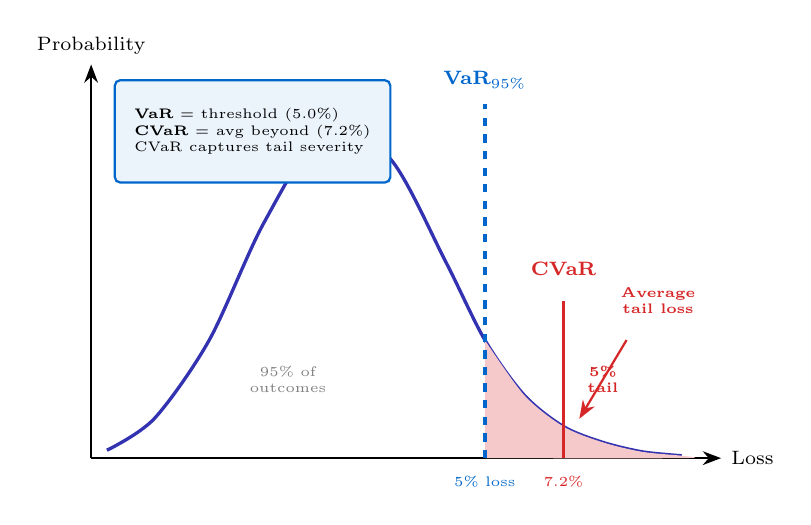
\begin{tikzpicture}
  % Axes
  \draw[-{Stealth}, thick] (0,0) -- (8.0,0) node[right, font=\scriptsize] {Loss};
  \draw[-{Stealth}, thick] (0,0) -- (0,5.0) node[above, font=\scriptsize] {Probability};

  % Distribution curve (bell-like, slightly skewed)
  \draw[mlpurple, very thick, smooth] plot coordinates {(0.2,0.1) (0.8,0.5) (1.5,1.5) (2.2,3.0) (3.0,4.2) (3.8,3.8) (4.5,2.5) (5.0,1.5) (5.5,0.8) (6.0,0.4) (6.5,0.2) (7.0,0.08) (7.5,0.03)};

  % Shaded tail beyond VaR
  \fill[mlred!25, smooth] plot coordinates {(5.0,1.5) (5.5,0.8) (6.0,0.4) (6.5,0.2) (7.0,0.08) (7.5,0.03) (7.5,0) (5.0,0)} -- cycle;

  % VaR line
  \draw[mlblue, very thick, dashed] (5.0,0) -- (5.0,4.5);
  \node[font=\scriptsize\bfseries, text=mlblue, align=center] at (5.0,4.8) {VaR$_{95\%}$};
  \node[font=\tiny, text=mlblue] at (5.0,-0.3) {5\% loss};

  % CVaR marker
  \draw[mlred, very thick] (6.0,0) -- (6.0,2.0);
  \node[font=\scriptsize\bfseries, text=mlred, align=center] at (6.0,2.4) {CVaR};
  \node[font=\tiny, text=mlred] at (6.0,-0.3) {7.2\%};

  % Annotation arrow for tail
  \draw[-{Stealth}, thick, mlred] (6.8,1.5) -- (6.2,0.5);
  \node[font=\tiny\bfseries, text=mlred, align=center] at (7.2,2.0) {Average\\tail loss};

  % 95% region label
  \node[font=\tiny, text=mlgray, align=center] at (2.5,1.0) {95\% of\\outcomes};

  % 5% tail label
  \node[font=\tiny\bfseries, text=mlred, align=center] at (6.5,1.0) {5\%\\tail};

  % Comparison box
  \fill[mlblue!8] (0.3,3.5) rectangle (3.8,4.8);
  \draw[mlblue, thick, rounded corners=2pt] (0.3,3.5) rectangle (3.8,4.8);
  \node[font=\tiny, align=left] at (2.05,4.15) {\textbf{VaR} = threshold (5.0\%)\\\textbf{CVaR} = avg beyond (7.2\%)\\CVaR captures tail severity};
\end{tikzpicture}
\end{columns}
\bottomnote{CVaR = Expected Shortfall = average loss beyond VaR | Sub-additive (coherent risk measure) | Basel III/IV standard | Always $\geq$ VaR at same confidence}
\end{frame}

% Frame 32: Sharpe Ratio & Risk-Adjusted Returns
\begin{frame}{Sharpe Ratio \& Risk-Adjusted Returns}
\begin{columns}[T]
\column{0.40\textwidth}
\begin{block}{Sharpe Ratio Formula}
$$S = \frac{R_p - R_f}{\sigma_p}$$
\begin{itemize}\setlength{\itemsep}{2pt}
  \item $R_p$ = portfolio return (annualised)
  \item $R_f$ = risk-free rate (T-bills, $\approx$4--5\%)
  \item $\sigma_p$ = portfolio volatility (annualised)
\end{itemize}
\end{block}
\vspace{2mm}
\begin{block}{Interpretation}
\begin{itemize}\setlength{\itemsep}{2pt}
  \item $S < 0$: Worse than risk-free
  \item $0 < S < 1$: Positive but mediocre
  \item $1 < S < 2$: Good risk-adjusted return
  \item $S > 2$: Very good (rare in crypto)
  \item $S > 3$: Exceptional or likely overfitted
\end{itemize}
\end{block}
\column{0.60\textwidth}
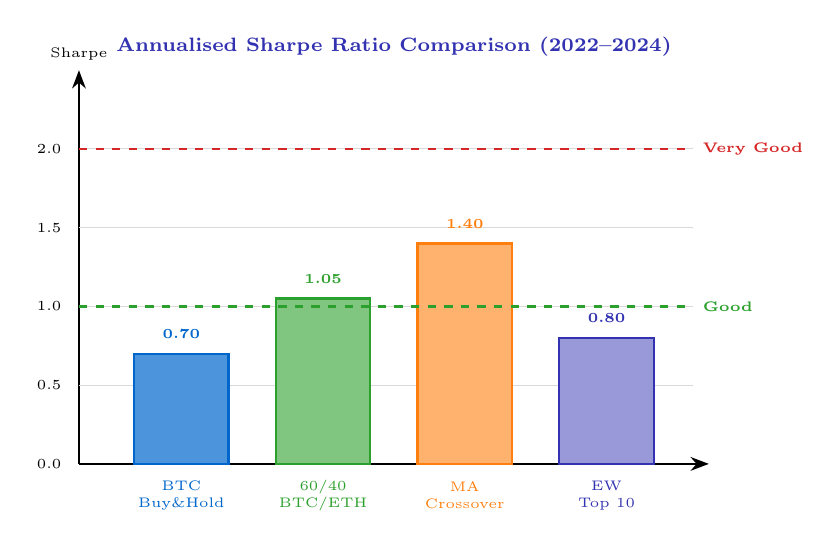
\begin{tikzpicture}
  % Title
  \node[font=\scriptsize\bfseries, text=mlpurple] at (4.5,5.8) {Annualised Sharpe Ratio Comparison (2022--2024)};

  % Axes
  \draw[-{Stealth}, thick] (0.5,0.5) -- (8.5,0.5) node[right, font=\tiny] {};
  \draw[-{Stealth}, thick] (0.5,0.5) -- (0.5,5.5) node[above, font=\tiny] {Sharpe};

  % Y-axis labels
  \node[font=\tiny, left] at (0.4,0.5) {0.0};
  \draw[mlgray!30] (0.5,1.5) -- (8.3,1.5);
  \node[font=\tiny, left] at (0.4,1.5) {0.5};
  \draw[mlgray!30] (0.5,2.5) -- (8.3,2.5);
  \node[font=\tiny, left] at (0.4,2.5) {1.0};
  \draw[mlgray!30] (0.5,3.5) -- (8.3,3.5);
  \node[font=\tiny, left] at (0.4,3.5) {1.5};
  \draw[mlgray!30] (0.5,4.5) -- (8.3,4.5);
  \node[font=\tiny, left] at (0.4,4.5) {2.0};

  % Bar 1: Buy-and-hold BTC
  \fill[mlblue!70] (1.2,0.5) rectangle (2.4,1.9);
  \draw[mlblue, thick] (1.2,0.5) rectangle (2.4,1.9);
  \node[font=\tiny\bfseries, text=mlblue] at (1.8,2.15) {0.70};
  \node[font=\tiny, text=mlblue, align=center] at (1.8,0.1) {BTC\\Buy\&Hold};

  % Bar 2: 60/40 BTC/ETH
  \fill[mlgreen!60] (3.0,0.5) rectangle (4.2,2.6);
  \draw[mlgreen, thick] (3.0,0.5) rectangle (4.2,2.6);
  \node[font=\tiny\bfseries, text=mlgreen] at (3.6,2.85) {1.05};
  \node[font=\tiny, text=mlgreen, align=center] at (3.6,0.1) {60/40\\BTC/ETH};

  % Bar 3: MA Crossover
  \fill[mlorange!60] (4.8,0.5) rectangle (6.0,3.3);
  \draw[mlorange, thick] (4.8,0.5) rectangle (6.0,3.3);
  \node[font=\tiny\bfseries, text=mlorange] at (5.4,3.55) {1.40};
  \node[font=\tiny, text=mlorange, align=center] at (5.4,0.1) {MA\\Crossover};

  % Bar 4: Equal-weight Top 10
  \fill[mlpurple!50] (6.6,0.5) rectangle (7.8,2.1);
  \draw[mlpurple, thick] (6.6,0.5) rectangle (7.8,2.1);
  \node[font=\tiny\bfseries, text=mlpurple] at (7.2,2.35) {0.80};
  \node[font=\tiny, text=mlpurple, align=center] at (7.2,0.1) {EW\\Top 10};

  % Reference lines
  \draw[mlgreen, thick, dashed] (0.5,2.5) -- (8.3,2.5);
  \node[font=\tiny\bfseries, text=mlgreen, right] at (8.3,2.5) {Good};
  \draw[mlred, thick, dashed] (0.5,4.5) -- (8.3,4.5);
  \node[font=\tiny\bfseries, text=mlred, right] at (8.3,4.5) {Very Good};
\end{tikzpicture}
\end{columns}
\bottomnote{Sharpe = excess return per unit risk | $>$1 good, $>$2 very good | Penalises both upside and downside volatility | Use Sortino for asymmetric returns}
\end{frame}

% Frame 33: Sortino Ratio & Downside Risk
\begin{frame}{Sortino Ratio \& Downside Risk}
\begin{columns}[T]
\column{0.45\textwidth}
\begin{block}{Sortino Ratio Formula}
$$\text{Sortino} = \frac{R_p - R_f}{\sigma_{\text{downside}}}$$
\begin{itemize}\setlength{\itemsep}{2pt}
  \item $\sigma_{\text{downside}}$ = standard deviation of \emph{negative} returns only
  \item Does not penalise upside volatility
  \item More appropriate for skewed return distributions
\end{itemize}
\end{block}
\vspace{2mm}
\begin{block}{Why It Matters for Crypto}
\begin{itemize}\setlength{\itemsep}{2pt}
  \item Crypto returns are \textbf{positively skewed}: large upside moves are common
  \item Sharpe penalises these equally to downside moves
  \item Sortino isolates \textbf{harmful volatility} from beneficial volatility
  \item Typical crypto: Sortino $>$ Sharpe (upside $>$ downside vol)
\end{itemize}
\end{block}
\column{0.55\textwidth}
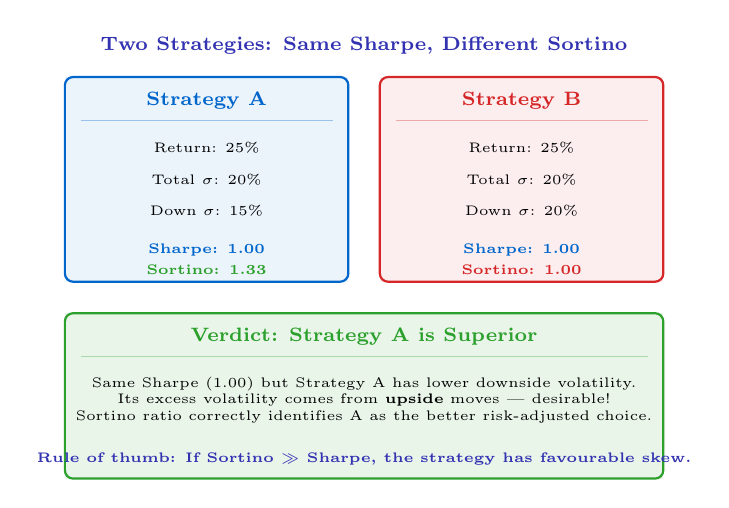
\begin{tikzpicture}
  % Title
  \node[font=\scriptsize\bfseries, text=mlpurple] at (4.0,5.8) {Two Strategies: Same Sharpe, Different Sortino};

  % Strategy A panel
  \fill[mlblue!8] (0.2,2.8) rectangle (3.8,5.4);
  \draw[mlblue, thick, rounded corners=3pt] (0.2,2.8) rectangle (3.8,5.4);
  \node[font=\scriptsize\bfseries, text=mlblue] at (2.0,5.1) {Strategy A};
  \draw[mlblue!40] (0.4,4.85) -- (3.6,4.85);
  \node[font=\tiny, align=left] at (2.0,4.5) {Return: 25\%};
  \node[font=\tiny, align=left] at (2.0,4.1) {Total $\sigma$: 20\%};
  \node[font=\tiny, align=left] at (2.0,3.7) {Down $\sigma$: 15\%};
  \node[font=\tiny\bfseries, text=mlblue] at (2.0,3.2) {Sharpe: 1.00};
  \node[font=\tiny\bfseries, text=mlgreen] at (2.0,2.95) {Sortino: 1.33};

  % Strategy B panel
  \fill[mlred!8] (4.2,2.8) rectangle (7.8,5.4);
  \draw[mlred, thick, rounded corners=3pt] (4.2,2.8) rectangle (7.8,5.4);
  \node[font=\scriptsize\bfseries, text=mlred] at (6.0,5.1) {Strategy B};
  \draw[mlred!40] (4.4,4.85) -- (7.6,4.85);
  \node[font=\tiny, align=left] at (6.0,4.5) {Return: 25\%};
  \node[font=\tiny, align=left] at (6.0,4.1) {Total $\sigma$: 20\%};
  \node[font=\tiny, align=left] at (6.0,3.7) {Down $\sigma$: 20\%};
  \node[font=\tiny\bfseries, text=mlblue] at (6.0,3.2) {Sharpe: 1.00};
  \node[font=\tiny\bfseries, text=mlred] at (6.0,2.95) {Sortino: 1.00};

  % Verdict box
  \fill[mlgreen!10] (0.2,0.3) rectangle (7.8,2.4);
  \draw[mlgreen, thick, rounded corners=3pt] (0.2,0.3) rectangle (7.8,2.4);
  \node[font=\scriptsize\bfseries, text=mlgreen] at (4.0,2.1) {Verdict: Strategy A is Superior};
  \draw[mlgreen!40] (0.4,1.85) -- (7.6,1.85);
  \node[font=\tiny, align=center] at (4.0,1.3) {Same Sharpe (1.00) but Strategy A has lower downside volatility.\\Its excess volatility comes from \textbf{upside} moves --- desirable!\\Sortino ratio correctly identifies A as the better risk-adjusted choice.};
  \node[font=\tiny\bfseries, text=mlpurple] at (4.0,0.55) {Rule of thumb: If Sortino $\gg$ Sharpe, the strategy has favourable skew.};
\end{tikzpicture}
\end{columns}
\bottomnote{Sortino: penalises only downside vol | Better for skewed crypto returns | If Sortino $\gg$ Sharpe, upside vol dominates | Always report both metrics}
\end{frame}

% Frame 34: Maximum Drawdown
\begin{frame}{Maximum Drawdown}
\begin{columns}[T]
\column{0.35\textwidth}
\begin{block}{Definition}
$$\text{MDD} = \frac{\text{Trough} - \text{Peak}}{\text{Peak}} \times 100\%$$
\begin{itemize}\setlength{\itemsep}{2pt}
  \item Largest peak-to-trough decline
  \item Measures worst-case loss experience
  \item Recovery time equally important
\end{itemize}
\end{block}
\vspace{1mm}
\begin{block}{Historical Crypto MDD}
\begin{itemize}\setlength{\itemsep}{2pt}
  \item \textbf{BTC 2017--18:} $-84\%$
  \item \textbf{BTC 2021--22:} $-77\%$
  \item \textbf{ETH 2022:} $-82\%$
  \item \textbf{LUNA 2022:} $-99.9\%$
  \item Recovery: 2--3 years typical for majors
\end{itemize}
\end{block}
\column{0.65\textwidth}
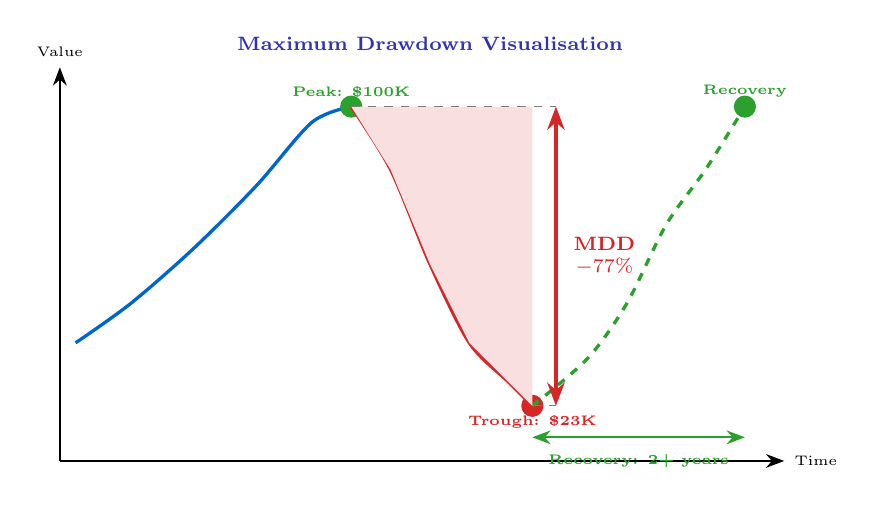
\begin{tikzpicture}
  % Title
  \node[font=\scriptsize\bfseries, text=mlpurple] at (5.0,5.8) {Maximum Drawdown Visualisation};

  % Axes
  \draw[-{Stealth}, thick] (0.3,0.5) -- (9.5,0.5) node[right, font=\tiny] {Time};
  \draw[-{Stealth}, thick] (0.3,0.5) -- (0.3,5.5) node[above, font=\tiny] {Value};

  % Portfolio value line
  \draw[mlblue, very thick, smooth] plot coordinates {(0.5,2.0) (1.2,2.5) (2.0,3.2) (2.8,4.0) (3.5,4.8) (4.0,5.0)};
  % Peak
  \fill[mlgreen] (4.0,5.0) circle (4pt);
  \node[font=\tiny\bfseries, text=mlgreen, above] at (4.0,5.0) {Peak: \$100K};

  % Decline
  \draw[mlred, very thick, smooth] plot coordinates {(4.0,5.0) (4.5,4.2) (5.0,3.0) (5.5,2.0) (6.0,1.5) (6.3,1.2)};
  % Trough
  \fill[mlred] (6.3,1.2) circle (4pt);
  \node[font=\tiny\bfseries, text=mlred, below] at (6.3,1.2) {Trough: \$23K};

  % Recovery
  \draw[mlgreen, very thick, smooth, dashed] plot coordinates {(6.3,1.2) (7.0,1.8) (7.5,2.5) (8.0,3.5) (8.5,4.2) (9.0,5.0)};
  \fill[mlgreen] (9.0,5.0) circle (4pt);
  \node[font=\tiny\bfseries, text=mlgreen, above] at (9.0,5.0) {Recovery};

  % Drawdown shading
  \fill[mlred!15] (4.0,5.0) -- (4.5,4.2) -- (5.0,3.0) -- (5.5,2.0) -- (6.0,1.5) -- (6.3,1.2) -- (6.3,5.0) -- cycle;

  % MDD arrow
  \draw[{Stealth}-{Stealth}, very thick, mlred] (6.6,5.0) -- (6.6,1.2);
  \node[font=\scriptsize\bfseries, text=mlred, right, align=center] at (6.7,3.1) {MDD\\$-77\%$};

  % Peak line
  \draw[mlgray, thin, dashed] (4.0,5.0) -- (6.6,5.0);
  \draw[mlgray, thin, dashed] (6.3,1.2) -- (6.6,1.2);

  % Recovery time
  \draw[{Stealth}-{Stealth}, thick, mlgreen] (6.3,0.8) -- (9.0,0.8);
  \node[font=\tiny\bfseries, text=mlgreen, align=center] at (7.65,0.5) {Recovery: 2+ years};
\end{tikzpicture}
\end{columns}
\bottomnote{MDD: worst peak-to-trough loss | BTC historically $-$77\% to $-$84\% | Recovery takes years | Critical metric for investor psychology and fund survival}
\end{frame}

% Frame 35: Position Sizing
\begin{frame}{Position Sizing}
\begin{columns}[T]
\column{0.45\textwidth}
\begin{block}{Kelly Criterion}
$$f^{*} = \frac{p \cdot b - q}{b}$$
\begin{itemize}\setlength{\itemsep}{2pt}
  \item $f^{*}$ = optimal fraction of capital to bet
  \item $p$ = probability of winning
  \item $q = 1 - p$ = probability of losing
  \item $b$ = win/loss ratio (payoff odds)
\end{itemize}
\end{block}
\vspace{1mm}
\begin{block}{Worked Example}
\begin{itemize}\setlength{\itemsep}{2pt}
  \item Win rate $p = 0.55$, loss rate $q = 0.45$
  \item Win/loss ratio $b = 1.5$ (risk \$1 to make \$1.50)
  \item $f^{*} = \frac{0.55 \times 1.5 - 0.45}{1.5} = \frac{0.375}{1.5} = 0.25$
  \item \textbf{Full Kelly:} Bet 25\% of capital per trade
  \item \textbf{Half-Kelly:} Bet 12.5\% (safer in practice)
\end{itemize}
\end{block}
\column{0.55\textwidth}
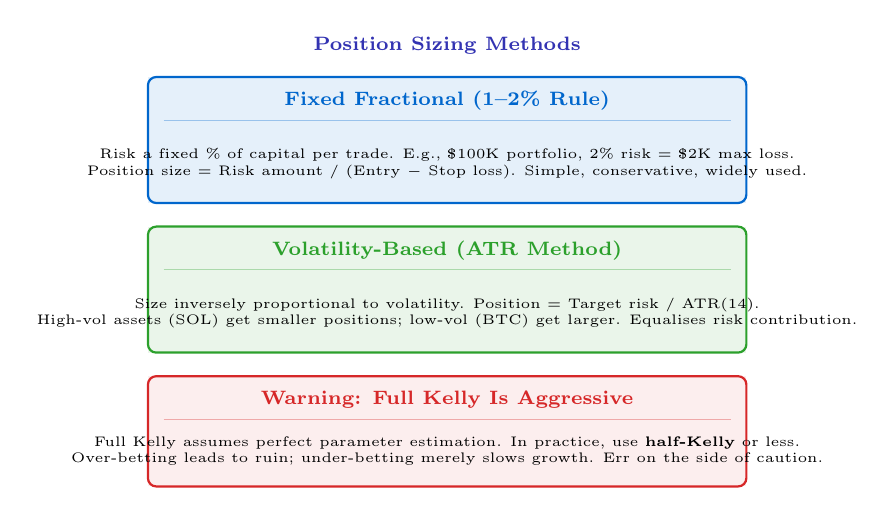
\begin{tikzpicture}
  % Title
  \node[font=\scriptsize\bfseries, text=mlpurple] at (4.0,5.8) {Position Sizing Methods};

  % Method 1: Fixed Fractional
  \fill[mlblue!10] (0.2,3.8) rectangle (7.8,5.4);
  \draw[mlblue, thick, rounded corners=3pt] (0.2,3.8) rectangle (7.8,5.4);
  \node[font=\scriptsize\bfseries, text=mlblue] at (4.0,5.1) {Fixed Fractional (1--2\% Rule)};
  \draw[mlblue!40] (0.4,4.85) -- (7.6,4.85);
  \node[font=\tiny, align=center] at (4.0,4.3) {Risk a fixed \% of capital per trade. E.g., \$100K portfolio, 2\% risk = \$2K max loss.\\Position size = Risk amount / (Entry $-$ Stop loss). Simple, conservative, widely used.};

  % Method 2: Volatility-Based
  \fill[mlgreen!10] (0.2,1.9) rectangle (7.8,3.5);
  \draw[mlgreen, thick, rounded corners=3pt] (0.2,1.9) rectangle (7.8,3.5);
  \node[font=\scriptsize\bfseries, text=mlgreen] at (4.0,3.2) {Volatility-Based (ATR Method)};
  \draw[mlgreen!40] (0.4,2.95) -- (7.6,2.95);
  \node[font=\tiny, align=center] at (4.0,2.4) {Size inversely proportional to volatility. Position = Target risk / ATR(14).\\High-vol assets (SOL) get smaller positions; low-vol (BTC) get larger. Equalises risk contribution.};

  % Warning box
  \fill[mlred!8] (0.2,0.2) rectangle (7.8,1.6);
  \draw[mlred, thick, rounded corners=3pt] (0.2,0.2) rectangle (7.8,1.6);
  \node[font=\scriptsize\bfseries, text=mlred] at (4.0,1.3) {Warning: Full Kelly Is Aggressive};
  \draw[mlred!40] (0.4,1.05) -- (7.6,1.05);
  \node[font=\tiny, align=center] at (4.0,0.65) {Full Kelly assumes perfect parameter estimation. In practice, use \textbf{half-Kelly} or less.\\Over-betting leads to ruin; under-betting merely slows growth. Err on the side of caution.};
\end{tikzpicture}
\end{columns}
\bottomnote{Kelly: optimal growth-rate sizing | Half-Kelly common in practice | Fixed fractional: 1--2\% per trade standard | Volatility-based: equalises risk across assets}
\end{frame}

% Frame 36: Portfolio Construction
\begin{frame}{Portfolio Construction}
\adjustbox{max width=\textwidth, max totalheight=6.5cm}{%
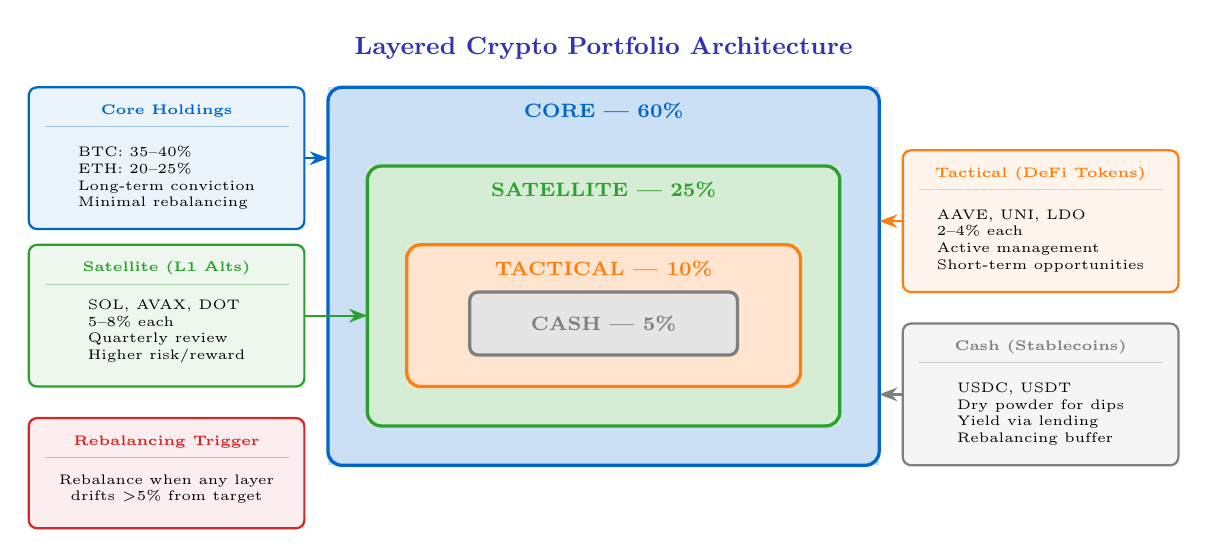
\begin{tikzpicture}
  % Title
  \node[font=\small\bfseries, text=mlpurple] at (7.5,6.3) {Layered Crypto Portfolio Architecture};

  % Core layer (innermost, largest)
  \fill[mlblue!20] (4.0,1.0) rectangle (11.0,5.8);
  \draw[mlblue, very thick, rounded corners=5pt] (4.0,1.0) rectangle (11.0,5.8);
  \node[font=\scriptsize\bfseries, text=mlblue] at (7.5,5.5) {CORE --- 60\%};

  % Satellite layer
  \fill[mlgreen!20] (4.5,1.5) rectangle (10.5,4.8);
  \draw[mlgreen, very thick, rounded corners=5pt] (4.5,1.5) rectangle (10.5,4.8);
  \node[font=\scriptsize\bfseries, text=mlgreen] at (7.5,4.5) {SATELLITE --- 25\%};

  % Tactical layer
  \fill[mlorange!20] (5.0,2.0) rectangle (10.0,3.8);
  \draw[mlorange, very thick, rounded corners=5pt] (5.0,2.0) rectangle (10.0,3.8);
  \node[font=\scriptsize\bfseries, text=mlorange] at (7.5,3.5) {TACTICAL --- 10\%};

  % Cash layer (innermost)
  \fill[mlgray!20] (5.8,2.4) rectangle (9.2,3.2);
  \draw[mlgray, very thick, rounded corners=3pt] (5.8,2.4) rectangle (9.2,3.2);
  \node[font=\scriptsize\bfseries, text=mlgray] at (7.5,2.8) {CASH --- 5\%};

  % Core details (left side)
  \fill[mlblue!8] (0.2,4.0) rectangle (3.7,5.8);
  \draw[mlblue, thick, rounded corners=3pt] (0.2,4.0) rectangle (3.7,5.8);
  \node[font=\tiny\bfseries, text=mlblue] at (1.95,5.5) {Core Holdings};
  \draw[mlblue!40] (0.4,5.3) -- (3.5,5.3);
  \node[font=\tiny, align=left] at (1.95,4.65) {BTC: 35--40\%\\ETH: 20--25\%\\Long-term conviction\\Minimal rebalancing};
  \draw[-{Stealth}, thick, mlblue] (3.7,4.9) -- (4.0,4.9);

  % Satellite details (left side)
  \fill[mlgreen!8] (0.2,2.0) rectangle (3.7,3.8);
  \draw[mlgreen, thick, rounded corners=3pt] (0.2,2.0) rectangle (3.7,3.8);
  \node[font=\tiny\bfseries, text=mlgreen] at (1.95,3.5) {Satellite (L1 Alts)};
  \draw[mlgreen!40] (0.4,3.3) -- (3.5,3.3);
  \node[font=\tiny, align=left] at (1.95,2.7) {SOL, AVAX, DOT\\5--8\% each\\Quarterly review\\Higher risk/reward};
  \draw[-{Stealth}, thick, mlgreen] (3.7,2.9) -- (4.5,2.9);

  % Tactical details (right side)
  \fill[mlorange!8] (11.3,3.2) rectangle (14.8,5.0);
  \draw[mlorange, thick, rounded corners=3pt] (11.3,3.2) rectangle (14.8,5.0);
  \node[font=\tiny\bfseries, text=mlorange] at (13.05,4.7) {Tactical (DeFi Tokens)};
  \draw[mlorange!40] (11.5,4.5) -- (14.6,4.5);
  \node[font=\tiny, align=left] at (13.05,3.85) {AAVE, UNI, LDO\\2--4\% each\\Active management\\Short-term opportunities};
  \draw[-{Stealth}, thick, mlorange] (11.3,4.1) -- (11.0,4.1);

  % Cash details (right side)
  \fill[mlgray!8] (11.3,1.0) rectangle (14.8,2.8);
  \draw[mlgray, thick, rounded corners=3pt] (11.3,1.0) rectangle (14.8,2.8);
  \node[font=\tiny\bfseries, text=mlgray] at (13.05,2.5) {Cash (Stablecoins)};
  \draw[mlgray!40] (11.5,2.3) -- (14.6,2.3);
  \node[font=\tiny, align=left] at (13.05,1.65) {USDC, USDT\\Dry powder for dips\\Yield via lending\\Rebalancing buffer};
  \draw[-{Stealth}, thick, mlgray] (11.3,1.9) -- (11.0,1.9);

  % Rebalancing trigger
  \fill[mlred!8] (0.2,0.2) rectangle (3.7,1.6);
  \draw[mlred, thick, rounded corners=3pt] (0.2,0.2) rectangle (3.7,1.6);
  \node[font=\tiny\bfseries, text=mlred] at (1.95,1.3) {Rebalancing Trigger};
  \draw[mlred!40] (0.4,1.1) -- (3.5,1.1);
  \node[font=\tiny, align=center] at (1.95,0.7) {Rebalance when any layer\\drifts $>$5\% from target};
\end{tikzpicture}%
}%
\bottomnote{Core-satellite: 60\% BTC+ETH, 25\% L1 alts, 10\% DeFi tactical, 5\% stablecoin cash | Rebalance on $>$5\% drift | Layered approach manages risk exposure}
\end{frame}

% Frame 37: Risk Monitoring Dashboard
\begin{frame}{Risk Monitoring Dashboard}
\adjustbox{max width=\textwidth, max totalheight=6.5cm}{%
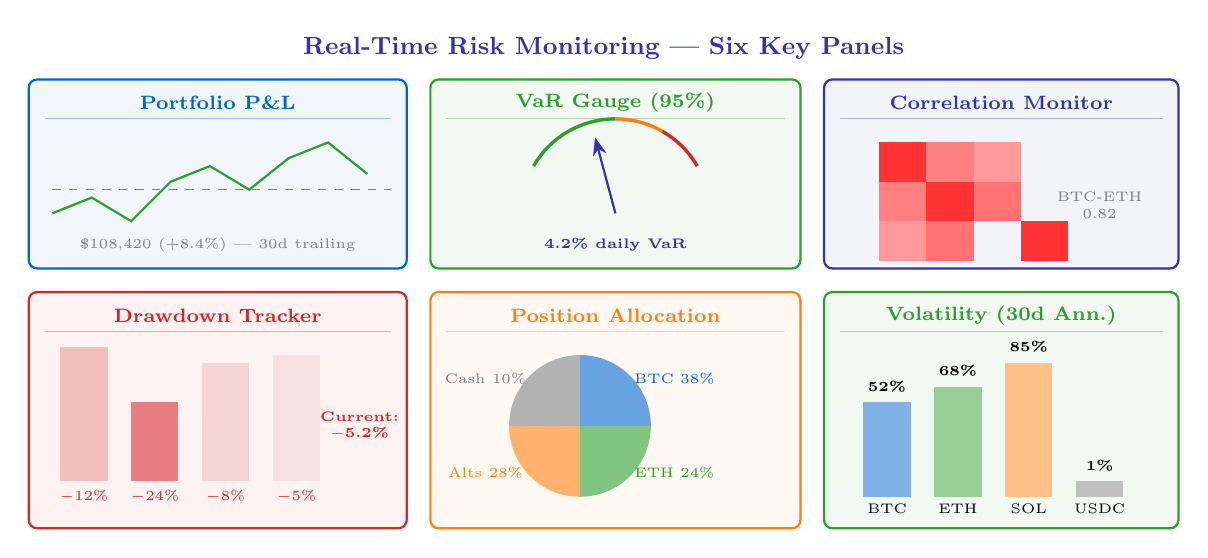
\begin{tikzpicture}
  % Title
  \node[font=\small\bfseries, text=mlpurple] at (7.5,6.3) {Real-Time Risk Monitoring --- Six Key Panels};

  % Panel 1: P&L Chart (top-left)
  \fill[mlblue!6] (0.2,3.5) rectangle (5.0,5.9);
  \draw[mlblue, thick, rounded corners=3pt] (0.2,3.5) rectangle (5.0,5.9);
  \node[font=\scriptsize\bfseries, text=mlblue] at (2.6,5.6) {Portfolio P\&L};
  \draw[mlblue!40] (0.4,5.4) -- (4.8,5.4);
  % Mini P&L line
  \draw[mlgreen, thick] (0.5,4.2) -- (1.0,4.4) -- (1.5,4.1) -- (2.0,4.6) -- (2.5,4.8) -- (3.0,4.5) -- (3.5,4.9) -- (4.0,5.1) -- (4.5,4.7);
  \draw[mlgray, thin, dashed] (0.5,4.5) -- (4.8,4.5);
  \node[font=\tiny, text=mlgray] at (2.6,3.8) {\$108,420 (+8.4\%) | 30d trailing};

  % Panel 2: VaR Gauge (top-center)
  \fill[mlgreen!6] (5.3,3.5) rectangle (10.0,5.9);
  \draw[mlgreen, thick, rounded corners=3pt] (5.3,3.5) rectangle (10.0,5.9);
  \node[font=\scriptsize\bfseries, text=mlgreen] at (7.65,5.6) {VaR Gauge (95\%)};
  \draw[mlgreen!40] (5.5,5.4) -- (9.8,5.4);
  % Gauge arc
  \draw[mlgray!40, very thick] (7.65,4.2) ++(150:1.2) arc (150:30:1.2);
  \draw[mlgreen, very thick] (7.65,4.2) ++(150:1.2) arc (150:90:1.2);
  \draw[mlorange, very thick] (7.65,4.2) ++(90:1.2) arc (90:60:1.2);
  \draw[mlred, very thick] (7.65,4.2) ++(60:1.2) arc (60:30:1.2);
  % Needle
  \draw[mlpurple, thick, -{Stealth}] (7.65,4.2) -- ++(105:1.0);
  \node[font=\tiny\bfseries, text=mlpurple] at (7.65,3.8) {4.2\% daily VaR};

  % Panel 3: Mini Correlation Heatmap (top-right)
  \fill[mlpurple!6] (10.3,3.5) rectangle (14.8,5.9);
  \draw[mlpurple, thick, rounded corners=3pt] (10.3,3.5) rectangle (14.8,5.9);
  \node[font=\scriptsize\bfseries, text=mlpurple] at (12.55,5.6) {Correlation Monitor};
  \draw[mlpurple!40] (10.5,5.4) -- (14.6,5.4);
  % 3x3 mini heatmap
  \fill[red!80] (11.0,4.6) rectangle (11.6,5.1);
  \fill[red!50] (11.6,4.6) rectangle (12.2,5.1);
  \fill[red!40] (12.2,4.6) rectangle (12.8,5.1);
  \fill[red!50] (11.0,4.1) rectangle (11.6,4.6);
  \fill[red!80] (11.6,4.1) rectangle (12.2,4.6);
  \fill[red!55] (12.2,4.1) rectangle (12.8,4.6);
  \fill[red!40] (11.0,3.6) rectangle (11.6,4.1);
  \fill[red!55] (11.6,3.6) rectangle (12.2,4.1);
  \fill[red!80] (12.8,3.6) rectangle (13.4,4.1);
  \node[font=\tiny, text=mlgray, align=center] at (13.8,4.3) {BTC-ETH\\0.82};

  % Panel 4: Drawdown Tracker (bottom-left)
  \fill[mlred!6] (0.2,0.2) rectangle (5.0,3.2);
  \draw[mlred, thick, rounded corners=3pt] (0.2,0.2) rectangle (5.0,3.2);
  \node[font=\scriptsize\bfseries, text=mlred] at (2.6,2.9) {Drawdown Tracker};
  \draw[mlred!40] (0.4,2.7) -- (4.8,2.7);
  % Mini drawdown bars
  \fill[mlred!30] (0.6,0.8) rectangle (1.2,2.5);
  \node[font=\tiny, text=mlred] at (0.9,0.6) {$-$12\%};
  \fill[mlred!60] (1.5,0.8) rectangle (2.1,1.8);
  \node[font=\tiny, text=mlred] at (1.8,0.6) {$-$24\%};
  \fill[mlred!20] (2.4,0.8) rectangle (3.0,2.3);
  \node[font=\tiny, text=mlred] at (2.7,0.6) {$-$8\%};
  \fill[mlred!15] (3.3,0.8) rectangle (3.9,2.4);
  \node[font=\tiny, text=mlred] at (3.6,0.6) {$-$5\%};
  \node[font=\tiny\bfseries, text=mlred, align=center] at (4.4,1.5) {Current:\\$-$5.2\%};

  % Panel 5: Position Allocation Pie (bottom-center)
  \fill[mlorange!6] (5.3,0.2) rectangle (10.0,3.2);
  \draw[mlorange, thick, rounded corners=3pt] (5.3,0.2) rectangle (10.0,3.2);
  \node[font=\scriptsize\bfseries, text=mlorange] at (7.65,2.9) {Position Allocation};
  \draw[mlorange!40] (5.5,2.7) -- (9.8,2.7);
  % Pie chart approximation
  \fill[mlblue!60] (7.2,1.5) -- (7.2,2.4) arc (90:0:0.9) -- cycle;
  \fill[mlgreen!60] (7.2,1.5) -- (8.1,1.5) arc (0:-90:0.9) -- cycle;
  \fill[mlorange!60] (7.2,1.5) -- (7.2,0.6) arc (-90:-180:0.9) -- cycle;
  \fill[mlgray!60] (7.2,1.5) -- (6.3,1.5) arc (180:90:0.9) -- cycle;
  \node[font=\tiny, text=mlblue] at (8.4,2.1) {BTC 38\%};
  \node[font=\tiny, text=mlgreen] at (8.4,0.9) {ETH 24\%};
  \node[font=\tiny, text=mlorange] at (6.0,0.9) {Alts 28\%};
  \node[font=\tiny, text=mlgray] at (6.0,2.1) {Cash 10\%};

  % Panel 6: Volatility Indicator (bottom-right)
  \fill[mlgreen!6] (10.3,0.2) rectangle (14.8,3.2);
  \draw[mlgreen, thick, rounded corners=3pt] (10.3,0.2) rectangle (14.8,3.2);
  \node[font=\scriptsize\bfseries, text=mlgreen] at (12.55,2.9) {Volatility (30d Ann.)};
  \draw[mlgreen!40] (10.5,2.7) -- (14.6,2.7);
  % Mini vol bars
  \fill[mlblue!50] (10.8,0.6) rectangle (11.4,1.8);
  \node[font=\tiny] at (11.1,0.45) {BTC};
  \node[font=\tiny\bfseries] at (11.1,2.0) {52\%};
  \fill[mlgreen!50] (11.7,0.6) rectangle (12.3,2.0);
  \node[font=\tiny] at (12.0,0.45) {ETH};
  \node[font=\tiny\bfseries] at (12.0,2.2) {68\%};
  \fill[mlorange!50] (12.6,0.6) rectangle (13.2,2.3);
  \node[font=\tiny] at (12.9,0.45) {SOL};
  \node[font=\tiny\bfseries] at (12.9,2.5) {85\%};
  \fill[mlgray!50] (13.5,0.6) rectangle (14.1,0.8);
  \node[font=\tiny] at (13.8,0.45) {USDC};
  \node[font=\tiny\bfseries] at (13.8,1.0) {1\%};
\end{tikzpicture}%
}%
\bottomnote{6-panel dashboard: P\&L, VaR gauge, correlation, drawdown, allocation, volatility | Real-time monitoring essential for active crypto portfolio management}
\end{frame}

% Frame 38: Section 3 Summary
\begin{frame}{Section 3 Summary}
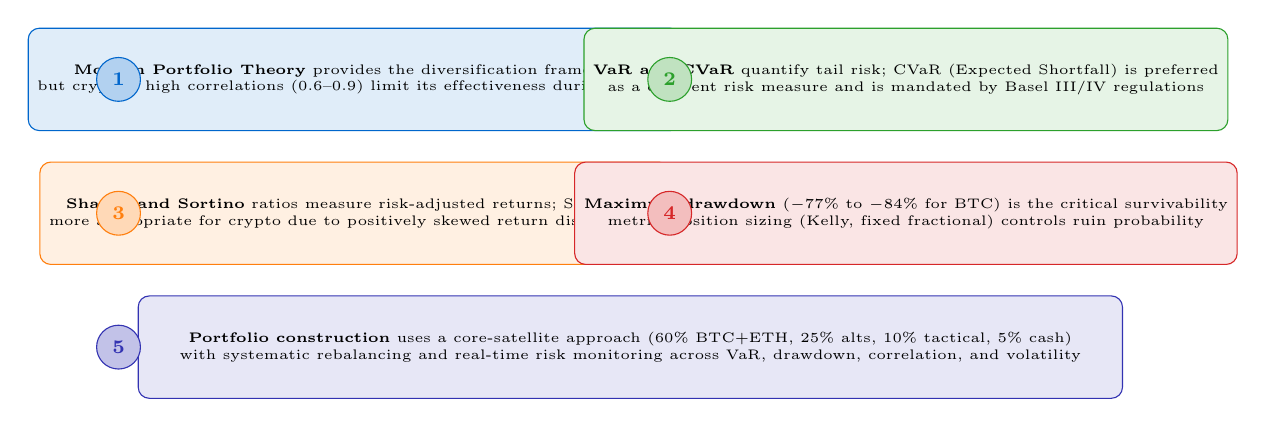
\begin{tikzpicture}
  \node[draw=mlblue, fill=mlblue!12, rounded corners=4pt, minimum width=5.5cm, minimum height=1.3cm, align=center, font=\tiny] (k1) at (4.0,5.0) {\textbf{Modern Portfolio Theory} provides the diversification framework,\\but crypto's high correlations (0.6--0.9) limit its effectiveness during crashes};
  \node[circle, draw=mlblue, fill=mlblue!30, minimum size=0.55cm, font=\scriptsize\bfseries, text=mlblue] at (1.0,5.0) {1};

  \node[draw=mlgreen, fill=mlgreen!12, rounded corners=4pt, minimum width=5.5cm, minimum height=1.3cm, align=center, font=\tiny] (k2) at (11.0,5.0) {\textbf{VaR and CVaR} quantify tail risk; CVaR (Expected Shortfall) is preferred\\as a coherent risk measure and is mandated by Basel III/IV regulations};
  \node[circle, draw=mlgreen, fill=mlgreen!30, minimum size=0.55cm, font=\scriptsize\bfseries, text=mlgreen] at (8.0,5.0) {2};

  \node[draw=mlorange, fill=mlorange!12, rounded corners=4pt, minimum width=5.5cm, minimum height=1.3cm, align=center, font=\tiny] (k3) at (4.0,3.3) {\textbf{Sharpe and Sortino} ratios measure risk-adjusted returns; Sortino is\\more appropriate for crypto due to positively skewed return distributions};
  \node[circle, draw=mlorange, fill=mlorange!30, minimum size=0.55cm, font=\scriptsize\bfseries, text=mlorange] at (1.0,3.3) {3};

  \node[draw=mlred, fill=mlred!12, rounded corners=4pt, minimum width=5.5cm, minimum height=1.3cm, align=center, font=\tiny] (k4) at (11.0,3.3) {\textbf{Maximum drawdown} ($-$77\% to $-$84\% for BTC) is the critical survivability\\metric; position sizing (Kelly, fixed fractional) controls ruin probability};
  \node[circle, draw=mlred, fill=mlred!30, minimum size=0.55cm, font=\scriptsize\bfseries, text=mlred] at (8.0,3.3) {4};

  \node[draw=mlpurple, fill=mlpurple!12, rounded corners=4pt, minimum width=12.5cm, minimum height=1.3cm, align=center, font=\tiny] (k5) at (7.5,1.6) {\textbf{Portfolio construction} uses a core-satellite approach (60\% BTC+ETH, 25\% alts, 10\% tactical, 5\% cash)\\with systematic rebalancing and real-time risk monitoring across VaR, drawdown, correlation, and volatility};
  \node[circle, draw=mlpurple, fill=mlpurple!30, minimum size=0.55cm, font=\scriptsize\bfseries, text=mlpurple] at (1.0,1.6) {5};
\end{tikzpicture}
\bottomnote{Section 3 complete | 5 key takeaways | Proceed to Section 4: DEX vs CEX \& Market Manipulation}
\end{frame}

%% ============================================================
%% SECTION 4: DEX vs CEX & MARKET MANIPULATION
%% ============================================================
\section{DEX vs CEX \& Market Manipulation}

% Frame 39: Section 4 Divider
\begin{frame}{Section 4: DEX vs CEX \& Market Manipulation}
\begin{beamercolorbox}[sep=12pt,center,rounded=true,shadow=true]{palette quaternary}
  {\Large\bfseries Section 4: DEX vs CEX \& Market Manipulation}\\[4pt]
  {\normalsize Exchange architectures and the dark side of crypto markets}
\end{beamercolorbox}

\vspace{4mm}
\begin{columns}[T]
\column{0.55\textwidth}
\begin{block}{What You Will Learn}
\begin{itemize}\setlength{\itemsep}{2pt}
  \item CEX architecture, advantages, and catastrophic failure modes
  \item DEX mechanics: Automated Market Makers (AMMs) and on-chain CLOBs
  \item Manipulation tactics: wash trading, spoofing, and front-running
  \item MEV extraction and sandwich attacks on decentralised exchanges
\end{itemize}
\end{block}
\column{0.45\textwidth}
\begin{block}{Frames in This Section}
\begin{itemize}\setlength{\itemsep}{2pt}
  \item Frame 40: CEX Architecture
  \item Frame 41: CEX Risks \& Failures
  \item Frame 42: DEX Architecture \& AMMs
  \item Frame 43: CEX vs DEX Comparison
  \item Frame 44: Wash Trading
  \item Frame 45: Spoofing \& Layering
  \item Frame 46: Front-Running \& MEV
  \item Frame 47: Market Manipulation Detection
  \item Frame 48: Section 4 Summary
\end{itemize}
\end{block}
\end{columns}
\bottomnote{Section 4 of 5 | Frames 39--48 | Exchange architectures, manipulation tactics, and MEV in crypto markets}
\end{frame}

% Frame 40: CEX Architecture
\begin{frame}{CEX Architecture}
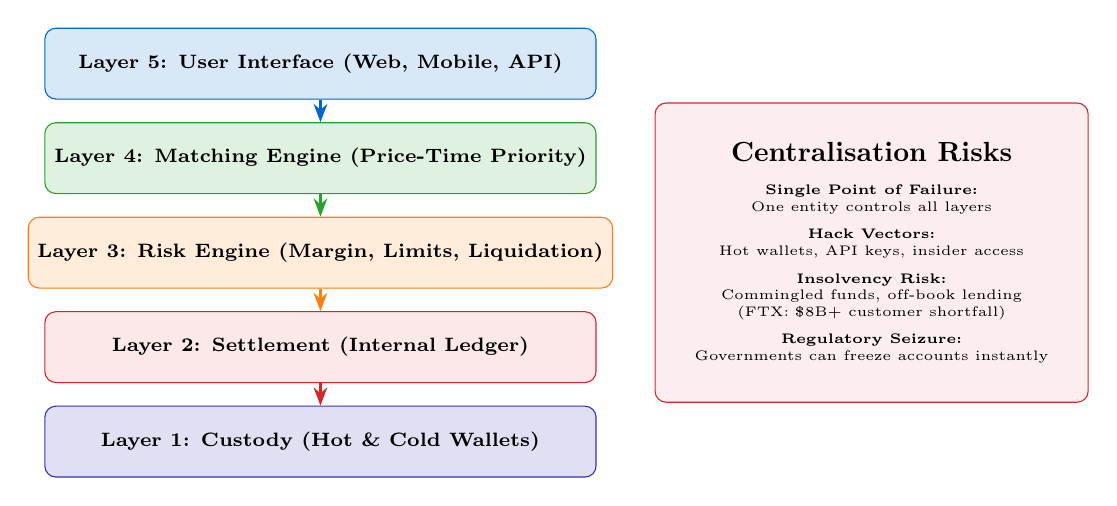
\begin{tikzpicture}
  % 5-layer stack
  \node[draw=mlblue, fill=mlblue!15, rounded corners=4pt, minimum width=7.0cm, minimum height=0.9cm, align=center, font=\scriptsize\bfseries] (l5) at (4.5,5.5) {Layer 5: User Interface (Web, Mobile, API)};
  \node[draw=mlgreen, fill=mlgreen!15, rounded corners=4pt, minimum width=7.0cm, minimum height=0.9cm, align=center, font=\scriptsize\bfseries] (l4) at (4.5,4.3) {Layer 4: Matching Engine (Price-Time Priority)};
  \node[draw=mlorange, fill=mlorange!15, rounded corners=4pt, minimum width=7.0cm, minimum height=0.9cm, align=center, font=\scriptsize\bfseries] (l3) at (4.5,3.1) {Layer 3: Risk Engine (Margin, Limits, Liquidation)};
  \node[draw=mlred, fill=mlred!10, rounded corners=4pt, minimum width=7.0cm, minimum height=0.9cm, align=center, font=\scriptsize\bfseries] (l2) at (4.5,1.9) {Layer 2: Settlement (Internal Ledger)};
  \node[draw=mlpurple, fill=mlpurple!15, rounded corners=4pt, minimum width=7.0cm, minimum height=0.9cm, align=center, font=\scriptsize\bfseries] (l1) at (4.5,0.7) {Layer 1: Custody (Hot \& Cold Wallets)};
  % Arrows between layers
  \draw[-{Stealth}, thick, mlblue] (l5.south) -- (l4.north);
  \draw[-{Stealth}, thick, mlgreen] (l4.south) -- (l3.north);
  \draw[-{Stealth}, thick, mlorange] (l3.south) -- (l2.north);
  \draw[-{Stealth}, thick, mlred] (l2.south) -- (l1.north);
  % Centralization risks on the right
  \node[draw=mlred, fill=mlred!8, rounded corners=4pt, minimum width=5.5cm, minimum height=3.8cm, align=center, font=\tiny] (risks) at (11.5,3.1) {%
    \textbf{\normalsize Centralisation Risks}\\[6pt]
    \textbf{Single Point of Failure:}\\
    One entity controls all layers\\[4pt]
    \textbf{Hack Vectors:}\\
    Hot wallets, API keys, insider access\\[4pt]
    \textbf{Insolvency Risk:}\\
    Commingled funds, off-book lending\\
    (FTX: \$8B+ customer shortfall)\\[4pt]
    \textbf{Regulatory Seizure:}\\
    Governments can freeze accounts instantly};
\end{tikzpicture}
\bottomnote{5-layer CEX stack: UI, matching, risk, settlement, custody | Centralisation creates single-point-of-failure risk across all layers}
\end{frame}

% Frame 41: CEX Risks & Failures
\begin{frame}{CEX Risks \& Failures}
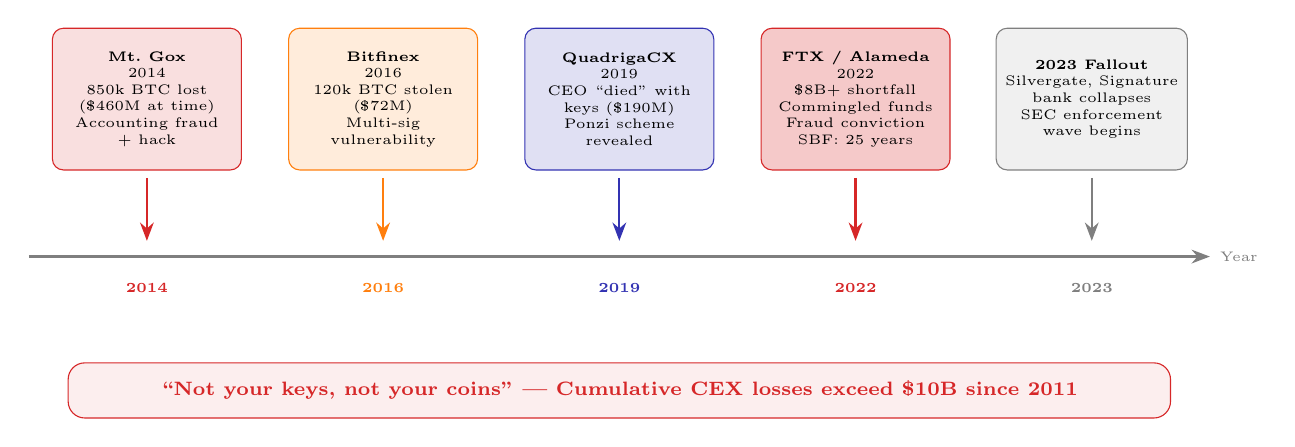
\begin{tikzpicture}
  % Timeline axis
  \draw[-{Stealth}, thick, mlgray] (0.0,2.5) -- (15.0,2.5) node[right, font=\tiny] {Year};
  % 2014 Mt. Gox
  \node[draw=mlred, fill=mlred!15, rounded corners=4pt, minimum width=2.4cm, minimum height=1.8cm, align=center, font=\tiny] (e1) at (1.5,4.5) {\textbf{Mt.\ Gox}\\2014\\850k BTC lost\\(\$460M at time)\\Accounting fraud\\+ hack};
  \draw[-{Stealth}, thick, mlred] (1.5,3.5) -- (1.5,2.7);
  \node[font=\tiny\bfseries, text=mlred] at (1.5,2.1) {2014};
  % 2016 Bitfinex
  \node[draw=mlorange, fill=mlorange!15, rounded corners=4pt, minimum width=2.4cm, minimum height=1.8cm, align=center, font=\tiny] (e2) at (4.5,4.5) {\textbf{Bitfinex}\\2016\\120k BTC stolen\\(\$72M)\\Multi-sig\\vulnerability};
  \draw[-{Stealth}, thick, mlorange] (4.5,3.5) -- (4.5,2.7);
  \node[font=\tiny\bfseries, text=mlorange] at (4.5,2.1) {2016};
  % 2019 QuadrigaCX
  \node[draw=mlpurple, fill=mlpurple!15, rounded corners=4pt, minimum width=2.4cm, minimum height=1.8cm, align=center, font=\tiny] (e3) at (7.5,4.5) {\textbf{QuadrigaCX}\\2019\\CEO ``died'' with\\keys (\$190M)\\Ponzi scheme\\revealed};
  \draw[-{Stealth}, thick, mlpurple] (7.5,3.5) -- (7.5,2.7);
  \node[font=\tiny\bfseries, text=mlpurple] at (7.5,2.1) {2019};
  % 2022 FTX
  \node[draw=mlred, fill=mlred!25, rounded corners=4pt, minimum width=2.4cm, minimum height=1.8cm, align=center, font=\tiny] (e4) at (10.5,4.5) {\textbf{FTX / Alameda}\\2022\\\$8B+ shortfall\\Commingled funds\\Fraud conviction\\SBF: 25 years};
  \draw[-{Stealth}, thick, mlred] (10.5,3.5) -- (10.5,2.7);
  \node[font=\tiny\bfseries, text=mlred] at (10.5,2.1) {2022};
  % 2023 Others
  \node[draw=mlgray, fill=mlgray!12, rounded corners=4pt, minimum width=2.4cm, minimum height=1.8cm, align=center, font=\tiny] (e5) at (13.5,4.5) {\textbf{2023 Fallout}\\Silvergate, Signature\\bank collapses\\SEC enforcement\\wave begins};
  \draw[-{Stealth}, thick, mlgray] (13.5,3.5) -- (13.5,2.7);
  \node[font=\tiny\bfseries, text=mlgray] at (13.5,2.1) {2023};
  % Bottom warning box
  \node[draw=mlred, fill=mlred!8, rounded corners=6pt, minimum width=14.0cm, minimum height=0.7cm, align=center, font=\scriptsize\bfseries, text=mlred] at (7.5,0.8) {``Not your keys, not your coins'' --- Cumulative CEX losses exceed \$10B since 2011};
\end{tikzpicture}
\bottomnote{CEX failure timeline: Mt.\ Gox to FTX | Cumulative losses exceed \$10B | Self-custody eliminates counterparty risk}
\end{frame}

% Frame 42: DEX Architecture & AMMs
\begin{frame}[fragile]{DEX Architecture \& AMMs}
\begin{columns}[T]
\column{0.50\textwidth}
\begin{lstlisting}[language=Python, caption={Constant Product AMM (x * y = k)}]
# Constant Product AMM (x * y = k)
def swap_exact_input(reserve_x,
                     reserve_y,
                     amount_in,
                     fee=0.003):
    amount_in_with_fee = (
        amount_in * (1 - fee))
    k = reserve_x * reserve_y

    new_reserve_x = (
        reserve_x + amount_in_with_fee)
    new_reserve_y = k / new_reserve_x
    amount_out = (
        reserve_y - new_reserve_y)
    return amount_out

# Example: ETH/USDC pool
# reserve_x = 1000 ETH
# reserve_y = 2,000,000 USDC
# k = 2,000,000,000
out = swap_exact_input(
    1000, 2_000_000, 10)
# out ~ 19,880 USDC (0.6% slippage)
\end{lstlisting}
\column{0.50\textwidth}
\begin{block}{Constant Product Invariant}
\begin{itemize}\setlength{\itemsep}{2pt}
  \item \textbf{Formula:} $x \cdot y = k$ (Uniswap V2)
  \item Price $P = \frac{y}{x}$; moves along hyperbola
  \item Larger pools $\Rightarrow$ lower slippage per trade
  \item Fee accrues to liquidity providers (LPs)
\end{itemize}
\end{block}
\vspace{2mm}
\begin{block}{Impermanent Loss}
\begin{itemize}\setlength{\itemsep}{2pt}
  \item LPs lose value vs.\ holding when prices diverge
  \item IL $= 2\frac{\sqrt{r}}{1+r} - 1$ where $r = \frac{P_1}{P_0}$
  \item 2$\times$ price change $\Rightarrow$ 5.7\% loss
  \item 5$\times$ price change $\Rightarrow$ 25.5\% loss
\end{itemize}
\end{block}
\vspace{2mm}
\begin{alertblock}{Concentrated Liquidity (Uniswap V3)}
\scriptsize LPs allocate capital to specific price ranges, increasing capital efficiency up to 4000$\times$ but amplifying impermanent loss within the range.
\end{alertblock}
\end{columns}
\bottomnote{Code Frame 4 | Constant product AMM: x*y=k | Impermanent loss is the hidden cost of passive liquidity provision}
\end{frame}

% Frame 43: CEX vs DEX Comparison
\begin{frame}{CEX vs DEX Comparison}
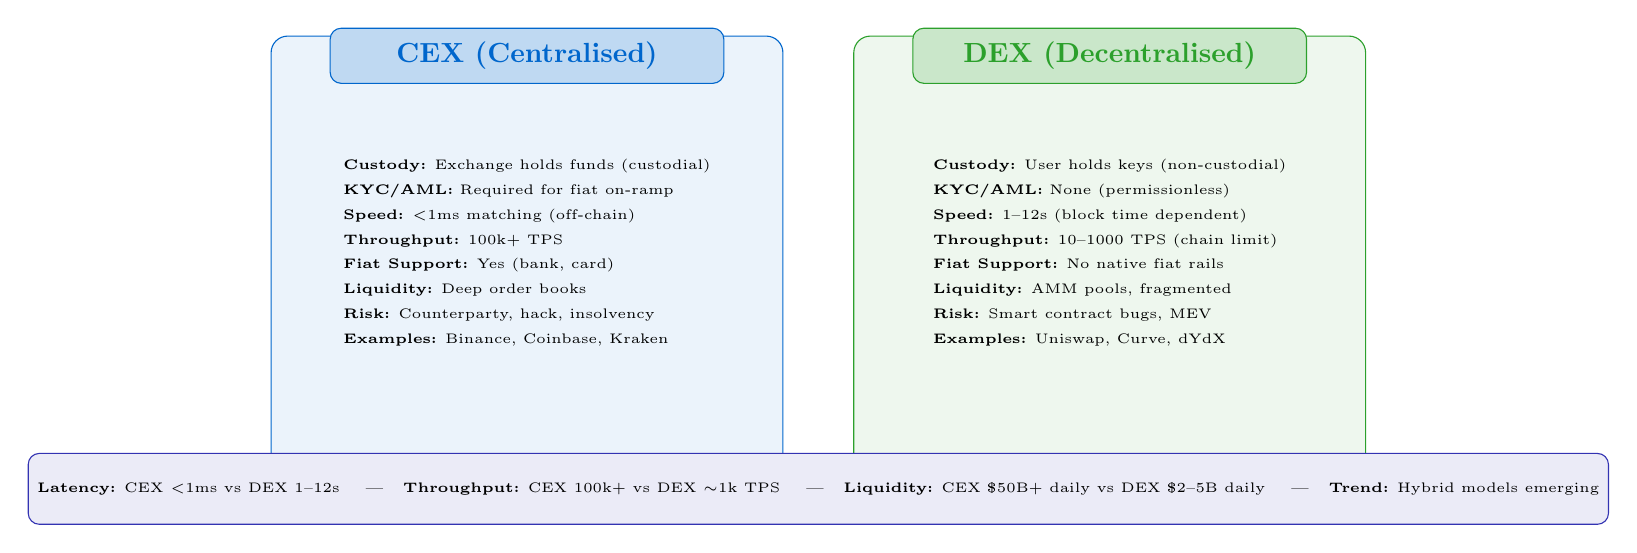
\begin{tikzpicture}
  % CEX panel
  \node[draw=mlblue, fill=mlblue!8, rounded corners=6pt, minimum width=6.5cm, minimum height=5.5cm, align=center] (cex) at (3.8,3.0) {};
  \node[draw=mlblue, fill=mlblue!25, rounded corners=4pt, minimum width=5.0cm, minimum height=0.7cm, align=center, font=\normalsize\bfseries, text=mlblue] at (3.8,5.5) {CEX (Centralised)};
  \node[align=left, font=\tiny] at (3.8,3.0) {%
    \textbf{Custody:} Exchange holds funds (custodial)\\[3pt]
    \textbf{KYC/AML:} Required for fiat on-ramp\\[3pt]
    \textbf{Speed:} $<$1ms matching (off-chain)\\[3pt]
    \textbf{Throughput:} 100k+ TPS\\[3pt]
    \textbf{Fiat Support:} Yes (bank, card)\\[3pt]
    \textbf{Liquidity:} Deep order books\\[3pt]
    \textbf{Risk:} Counterparty, hack, insolvency\\[3pt]
    \textbf{Examples:} Binance, Coinbase, Kraken};
  % DEX panel
  \node[draw=mlgreen, fill=mlgreen!8, rounded corners=6pt, minimum width=6.5cm, minimum height=5.5cm, align=center] (dex) at (11.2,3.0) {};
  \node[draw=mlgreen, fill=mlgreen!25, rounded corners=4pt, minimum width=5.0cm, minimum height=0.7cm, align=center, font=\normalsize\bfseries, text=mlgreen] at (11.2,5.5) {DEX (Decentralised)};
  \node[align=left, font=\tiny] at (11.2,3.0) {%
    \textbf{Custody:} User holds keys (non-custodial)\\[3pt]
    \textbf{KYC/AML:} None (permissionless)\\[3pt]
    \textbf{Speed:} 1--12s (block time dependent)\\[3pt]
    \textbf{Throughput:} 10--1000 TPS (chain limit)\\[3pt]
    \textbf{Fiat Support:} No native fiat rails\\[3pt]
    \textbf{Liquidity:} AMM pools, fragmented\\[3pt]
    \textbf{Risk:} Smart contract bugs, MEV\\[3pt]
    \textbf{Examples:} Uniswap, Curve, dYdX};
  % Comparison metrics at bottom
  \node[draw=mlpurple, fill=mlpurple!10, rounded corners=4pt, minimum width=13.5cm, minimum height=0.9cm, align=center, font=\tiny] at (7.5,0.0) {%
    \textbf{Latency:} CEX $<$1ms vs DEX 1--12s \quad|\quad
    \textbf{Throughput:} CEX 100k+ vs DEX $\sim$1k TPS \quad|\quad
    \textbf{Liquidity:} CEX \$50B+ daily vs DEX \$2--5B daily \quad|\quad
    \textbf{Trend:} Hybrid models emerging};
\end{tikzpicture}
\bottomnote{CEX vs DEX: custodial speed vs non-custodial sovereignty | Trade-off between performance and decentralisation}
\end{frame}

% Frame 44: Wash Trading
\begin{frame}{Wash Trading}
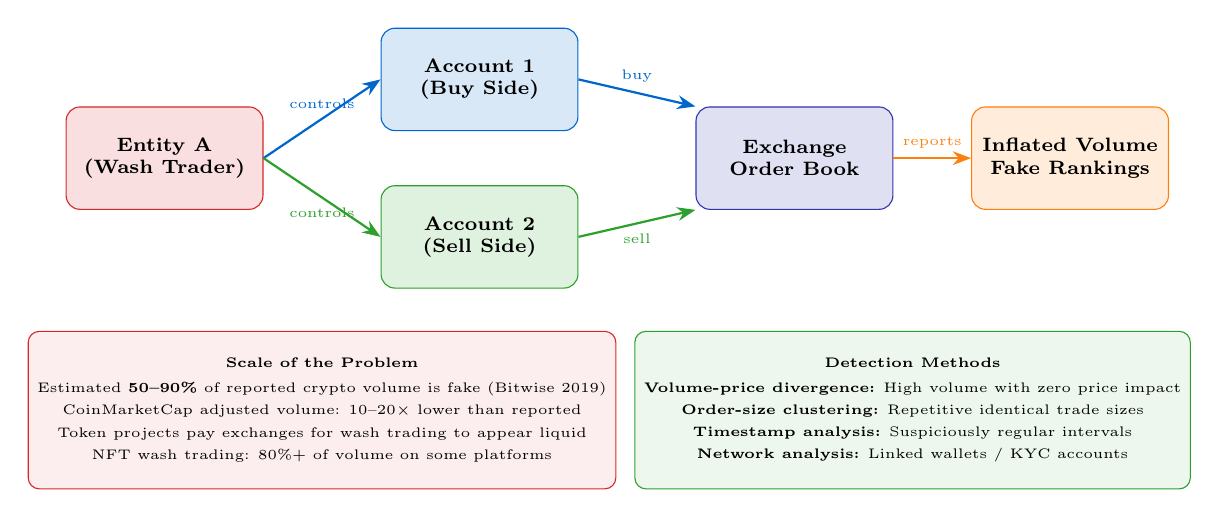
\begin{tikzpicture}
  % Flow: same entity buys/sells
  \node[draw=mlred, fill=mlred!15, rounded corners=5pt, minimum width=2.5cm, minimum height=1.3cm, align=center, font=\scriptsize\bfseries] (trader) at (1.5,4.5) {Entity A\\(Wash Trader)};
  \node[draw=mlblue, fill=mlblue!15, rounded corners=5pt, minimum width=2.5cm, minimum height=1.3cm, align=center, font=\scriptsize\bfseries] (acct1) at (5.5,5.5) {Account 1\\(Buy Side)};
  \node[draw=mlgreen, fill=mlgreen!15, rounded corners=5pt, minimum width=2.5cm, minimum height=1.3cm, align=center, font=\scriptsize\bfseries] (acct2) at (5.5,3.5) {Account 2\\(Sell Side)};
  \node[draw=mlpurple, fill=mlpurple!15, rounded corners=5pt, minimum width=2.5cm, minimum height=1.3cm, align=center, font=\scriptsize\bfseries] (exch) at (9.5,4.5) {Exchange\\Order Book};
  \node[draw=mlorange, fill=mlorange!15, rounded corners=5pt, minimum width=2.5cm, minimum height=1.3cm, align=center, font=\scriptsize\bfseries] (vol) at (13.0,4.5) {Inflated Volume\\Fake Rankings};
  % Arrows
  \draw[-{Stealth}, thick, mlblue] (trader.east) -- (acct1.west) node[midway, above, font=\tiny] {controls};
  \draw[-{Stealth}, thick, mlgreen] (trader.east) -- (acct2.west) node[midway, below, font=\tiny] {controls};
  \draw[-{Stealth}, thick, mlblue] (acct1.east) -- (exch.north west) node[midway, above, font=\tiny] {buy};
  \draw[-{Stealth}, thick, mlgreen] (acct2.east) -- (exch.south west) node[midway, below, font=\tiny] {sell};
  \draw[-{Stealth}, thick, mlorange] (exch.east) -- (vol.west) node[midway, above, font=\tiny] {reports};
  % Statistics box
  \node[draw=mlred, fill=mlred!8, rounded corners=4pt, minimum width=6.5cm, minimum height=2.0cm, align=center, font=\tiny] at (3.5,1.3) {%
    \textbf{Scale of the Problem}\\[3pt]
    Estimated \textbf{50--90\%} of reported crypto volume is fake (Bitwise 2019)\\[2pt]
    CoinMarketCap adjusted volume: 10--20$\times$ lower than reported\\[2pt]
    Token projects pay exchanges for wash trading to appear liquid\\[2pt]
    NFT wash trading: 80\%+ of volume on some platforms};
  % Detection methods box
  \node[draw=mlgreen, fill=mlgreen!8, rounded corners=4pt, minimum width=6.5cm, minimum height=2.0cm, align=center, font=\tiny] at (11.0,1.3) {%
    \textbf{Detection Methods}\\[3pt]
    \textbf{Volume-price divergence:} High volume with zero price impact\\[2pt]
    \textbf{Order-size clustering:} Repetitive identical trade sizes\\[2pt]
    \textbf{Timestamp analysis:} Suspiciously regular intervals\\[2pt]
    \textbf{Network analysis:} Linked wallets / KYC accounts};
\end{tikzpicture}
\bottomnote{Wash trading inflates 50--90\% of crypto volume | Detection: volume-price divergence, order clustering, timestamp regularity}
\end{frame}

% Frame 45: Spoofing & Layering
\begin{frame}{Spoofing \& Layering}
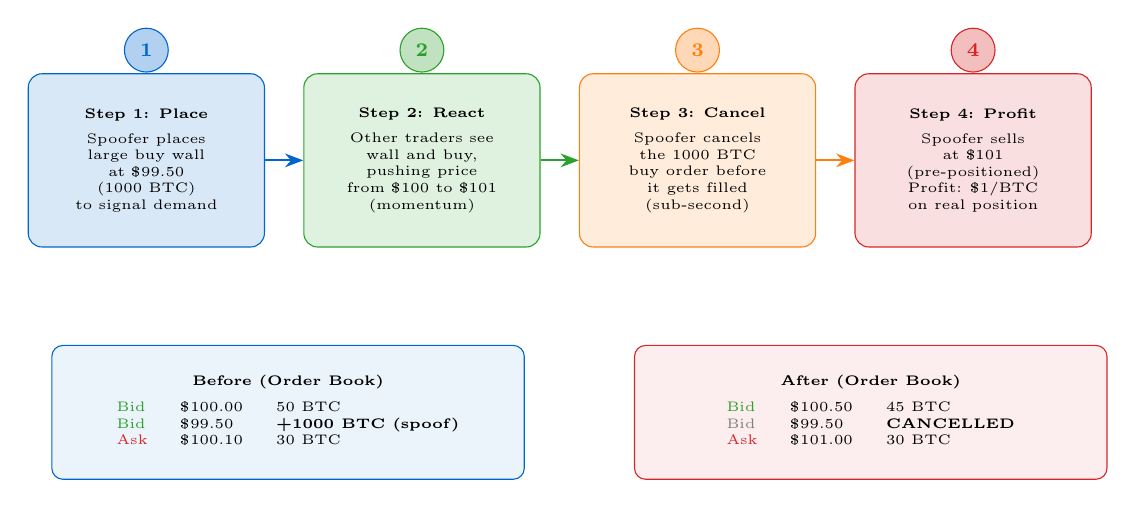
\begin{tikzpicture}
  % Step 1
  \node[draw=mlblue, fill=mlblue!15, rounded corners=5pt, minimum width=3.0cm, minimum height=2.2cm, align=center, font=\tiny] (s1) at (2.0,4.5) {\textbf{Step 1: Place}\\[3pt]Spoofer places\\large buy wall\\at \$99.50\\(1000 BTC)\\to signal demand};
  \node[circle, draw=mlblue, fill=mlblue!30, minimum size=0.55cm, font=\scriptsize\bfseries, text=mlblue] at (2.0,5.9) {1};
  % Step 2
  \node[draw=mlgreen, fill=mlgreen!15, rounded corners=5pt, minimum width=3.0cm, minimum height=2.2cm, align=center, font=\tiny] (s2) at (5.5,4.5) {\textbf{Step 2: React}\\[3pt]Other traders see\\wall and buy,\\pushing price\\from \$100 to \$101\\(momentum)};
  \node[circle, draw=mlgreen, fill=mlgreen!30, minimum size=0.55cm, font=\scriptsize\bfseries, text=mlgreen] at (5.5,5.9) {2};
  % Step 3
  \node[draw=mlorange, fill=mlorange!15, rounded corners=5pt, minimum width=3.0cm, minimum height=2.2cm, align=center, font=\tiny] (s3) at (9.0,4.5) {\textbf{Step 3: Cancel}\\[3pt]Spoofer cancels\\the 1000 BTC\\buy order before\\it gets filled\\(sub-second)};
  \node[circle, draw=mlorange, fill=mlorange!30, minimum size=0.55cm, font=\scriptsize\bfseries, text=mlorange] at (9.0,5.9) {3};
  % Step 4
  \node[draw=mlred, fill=mlred!15, rounded corners=5pt, minimum width=3.0cm, minimum height=2.2cm, align=center, font=\tiny] (s4) at (12.5,4.5) {\textbf{Step 4: Profit}\\[3pt]Spoofer sells\\at \$101\\(pre-positioned)\\Profit: \$1/BTC\\on real position};
  \node[circle, draw=mlred, fill=mlred!30, minimum size=0.55cm, font=\scriptsize\bfseries, text=mlred] at (12.5,5.9) {4};
  % Arrows
  \draw[-{Stealth}, thick, mlblue] (s1.east) -- (s2.west);
  \draw[-{Stealth}, thick, mlgreen] (s2.east) -- (s3.west);
  \draw[-{Stealth}, thick, mlorange] (s3.east) -- (s4.west);
  % Before/after order book
  \node[draw=mlblue, fill=mlblue!8, rounded corners=4pt, minimum width=6.0cm, minimum height=1.7cm, align=center, font=\tiny] at (3.8,1.3) {%
    \textbf{Before (Order Book)}\\[3pt]
    \begin{tabular}{lll}
    \textcolor{mlgreen}{Bid} & \$100.00 & 50 BTC \\
    \textcolor{mlgreen}{Bid} & \$99.50 & \textbf{+1000 BTC (spoof)} \\
    \textcolor{mlred}{Ask} & \$100.10 & 30 BTC \\
    \end{tabular}};
  \node[draw=mlred, fill=mlred!8, rounded corners=4pt, minimum width=6.0cm, minimum height=1.7cm, align=center, font=\tiny] at (11.2,1.3) {%
    \textbf{After (Order Book)}\\[3pt]
    \begin{tabular}{lll}
    \textcolor{mlgreen}{Bid} & \$100.50 & 45 BTC \\
    \textcolor{mlgray}{Bid} & \$99.50 & \textbf{CANCELLED} \\
    \textcolor{mlred}{Ask} & \$101.00 & 30 BTC \\
    \end{tabular}};
\end{tikzpicture}
\bottomnote{4-step spoofing cycle: place wall, trigger reaction, cancel, profit | Layering uses multiple price levels for greater deception}
\end{frame}

% Frame 46: Front-Running & MEV
\begin{frame}{Front-Running \& MEV}
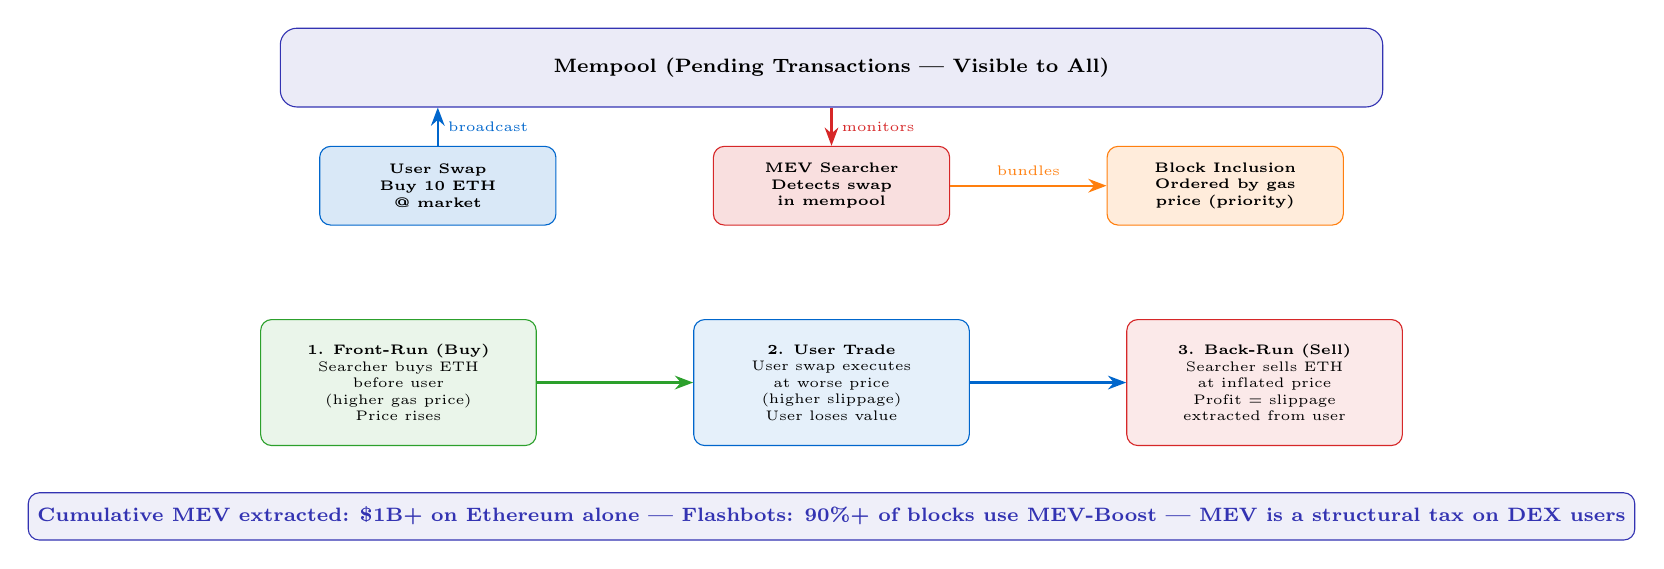
\begin{tikzpicture}
  % Mempool visualization
  \node[draw=mlpurple, fill=mlpurple!10, rounded corners=6pt, minimum width=14.0cm, minimum height=1.0cm, align=center, font=\scriptsize\bfseries] (mempool) at (7.5,6.0) {Mempool (Pending Transactions --- Visible to All)};
  % User transaction
  \node[draw=mlblue, fill=mlblue!15, rounded corners=4pt, minimum width=3.0cm, minimum height=1.0cm, align=center, font=\tiny\bfseries] (user) at (2.5,4.5) {User Swap\\Buy 10 ETH\\@ market};
  % Searcher sees
  \node[draw=mlred, fill=mlred!15, rounded corners=4pt, minimum width=3.0cm, minimum height=1.0cm, align=center, font=\tiny\bfseries] (searcher) at (7.5,4.5) {MEV Searcher\\Detects swap\\in mempool};
  % Sandwich result
  \node[draw=mlorange, fill=mlorange!15, rounded corners=4pt, minimum width=3.0cm, minimum height=1.0cm, align=center, font=\tiny\bfseries] (result) at (12.5,4.5) {Block Inclusion\\Ordered by gas\\price (priority)};
  \draw[-{Stealth}, thick, mlblue] (user.north) -- (user.north |- mempool.south) node[midway, right, font=\tiny] {broadcast};
  \draw[-{Stealth}, thick, mlred] (mempool.south -| searcher.north) -- (searcher.north) node[midway, right, font=\tiny] {monitors};
  \draw[-{Stealth}, thick, mlorange] (searcher.east) -- (result.west) node[midway, above, font=\tiny] {bundles};
  % Sandwich attack detail
  \node[draw=mlgreen, fill=mlgreen!10, rounded corners=4pt, minimum width=3.5cm, minimum height=1.6cm, align=center, font=\tiny] (step1) at (2.0,2.0) {\textbf{1. Front-Run (Buy)}\\Searcher buys ETH\\before user\\(higher gas price)\\Price rises};
  \node[draw=mlblue, fill=mlblue!10, rounded corners=4pt, minimum width=3.5cm, minimum height=1.6cm, align=center, font=\tiny] (step2) at (7.5,2.0) {\textbf{2. User Trade}\\User swap executes\\at worse price\\(higher slippage)\\User loses value};
  \node[draw=mlred, fill=mlred!10, rounded corners=4pt, minimum width=3.5cm, minimum height=1.6cm, align=center, font=\tiny] (step3) at (13.0,2.0) {\textbf{3. Back-Run (Sell)}\\Searcher sells ETH\\at inflated price\\Profit = slippage\\extracted from user};
  \draw[-{Stealth}, thick, mlgreen] (step1.east) -- (step2.west);
  \draw[-{Stealth}, thick, mlblue] (step2.east) -- (step3.west);
  % MEV stats
  \node[draw=mlpurple, fill=mlpurple!8, rounded corners=4pt, minimum width=14.0cm, minimum height=0.6cm, align=center, font=\scriptsize\bfseries, text=mlpurple] at (7.5,0.3) {Cumulative MEV extracted: \$1B+ on Ethereum alone | Flashbots: 90\%+ of blocks use MEV-Boost | MEV is a structural tax on DEX users};
\end{tikzpicture}
\bottomnote{Sandwich attack: front-run buy, user trade at worse price, back-run sell | MEV exceeds \$1B cumulative on Ethereum}
\end{frame}

% Frame 47: Market Manipulation Detection
\begin{frame}{Market Manipulation Detection}
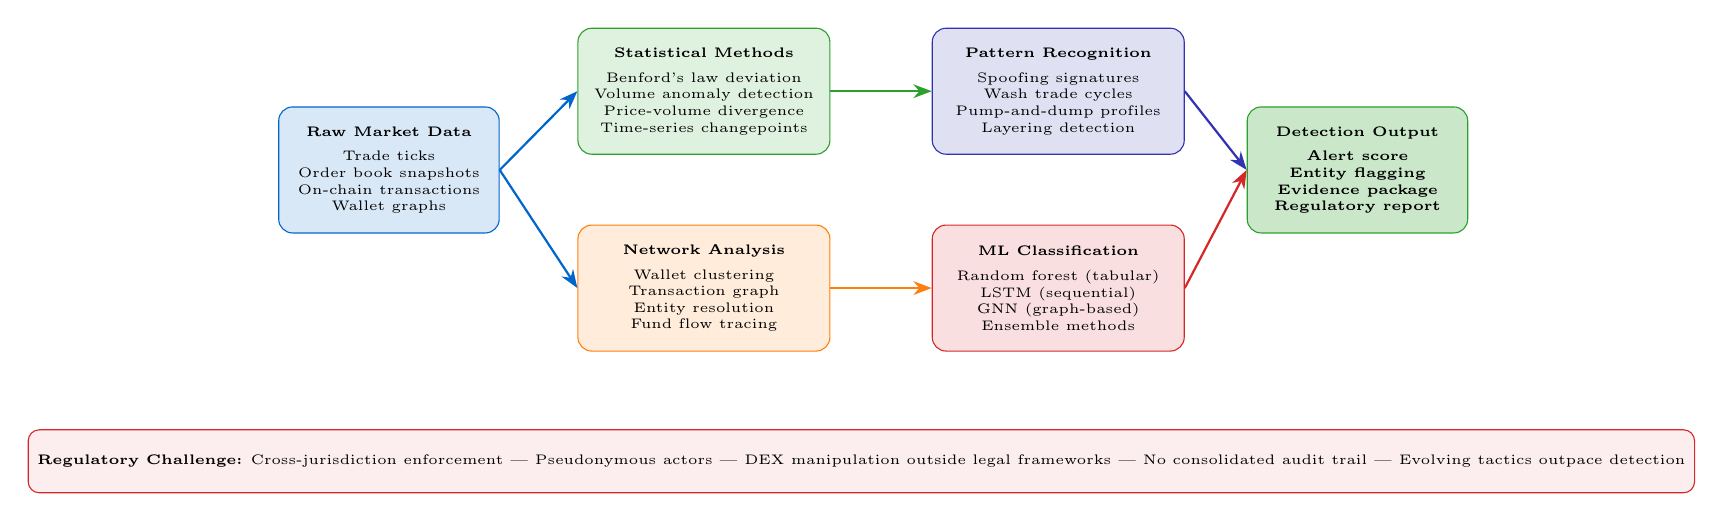
\begin{tikzpicture}
  % Input data
  \node[draw=mlblue, fill=mlblue!15, rounded corners=5pt, minimum width=2.8cm, minimum height=1.6cm, align=center, font=\tiny] (input) at (1.5,4.5) {\textbf{Raw Market Data}\\[3pt]Trade ticks\\Order book snapshots\\On-chain transactions\\Wallet graphs};
  % Statistical methods
  \node[draw=mlgreen, fill=mlgreen!15, rounded corners=5pt, minimum width=3.2cm, minimum height=1.6cm, align=center, font=\tiny] (stat) at (5.5,5.5) {\textbf{Statistical Methods}\\[3pt]Benford's law deviation\\Volume anomaly detection\\Price-volume divergence\\Time-series changepoints};
  % Network analysis
  \node[draw=mlorange, fill=mlorange!15, rounded corners=5pt, minimum width=3.2cm, minimum height=1.6cm, align=center, font=\tiny] (net) at (5.5,3.0) {\textbf{Network Analysis}\\[3pt]Wallet clustering\\Transaction graph\\Entity resolution\\Fund flow tracing};
  % Pattern recognition
  \node[draw=mlpurple, fill=mlpurple!15, rounded corners=5pt, minimum width=3.2cm, minimum height=1.6cm, align=center, font=\tiny] (pat) at (10.0,5.5) {\textbf{Pattern Recognition}\\[3pt]Spoofing signatures\\Wash trade cycles\\Pump-and-dump profiles\\Layering detection};
  % ML models
  \node[draw=mlred, fill=mlred!15, rounded corners=5pt, minimum width=3.2cm, minimum height=1.6cm, align=center, font=\tiny] (ml) at (10.0,3.0) {\textbf{ML Classification}\\[3pt]Random forest (tabular)\\LSTM (sequential)\\GNN (graph-based)\\Ensemble methods};
  % Output
  \node[draw=mlgreen, fill=mlgreen!25, rounded corners=5pt, minimum width=2.8cm, minimum height=1.6cm, align=center, font=\tiny\bfseries] (output) at (13.8,4.5) {\textbf{Detection Output}\\[3pt]Alert score\\Entity flagging\\Evidence package\\Regulatory report};
  % Arrows
  \draw[-{Stealth}, thick, mlblue] (input.east) -- (stat.west);
  \draw[-{Stealth}, thick, mlblue] (input.east) -- (net.west);
  \draw[-{Stealth}, thick, mlgreen] (stat.east) -- (pat.west);
  \draw[-{Stealth}, thick, mlorange] (net.east) -- (ml.west);
  \draw[-{Stealth}, thick, mlpurple] (pat.east) -- (output.west);
  \draw[-{Stealth}, thick, mlred] (ml.east) -- (output.west);
  % Regulatory challenge bar
  \node[draw=mlred, fill=mlred!8, rounded corners=4pt, minimum width=14.0cm, minimum height=0.8cm, align=center, font=\tiny] at (7.5,0.8) {%
    \textbf{Regulatory Challenge:} Cross-jurisdiction enforcement | Pseudonymous actors | DEX manipulation outside legal frameworks | No consolidated audit trail | Evolving tactics outpace detection};
\end{tikzpicture}
\bottomnote{Detection pipeline: raw data, statistical and network analysis, pattern recognition, ML classification | Cross-jurisdiction enforcement remains the core challenge}
\end{frame}

% Frame 48: Section 4 Summary
\begin{frame}{Section 4 Summary}
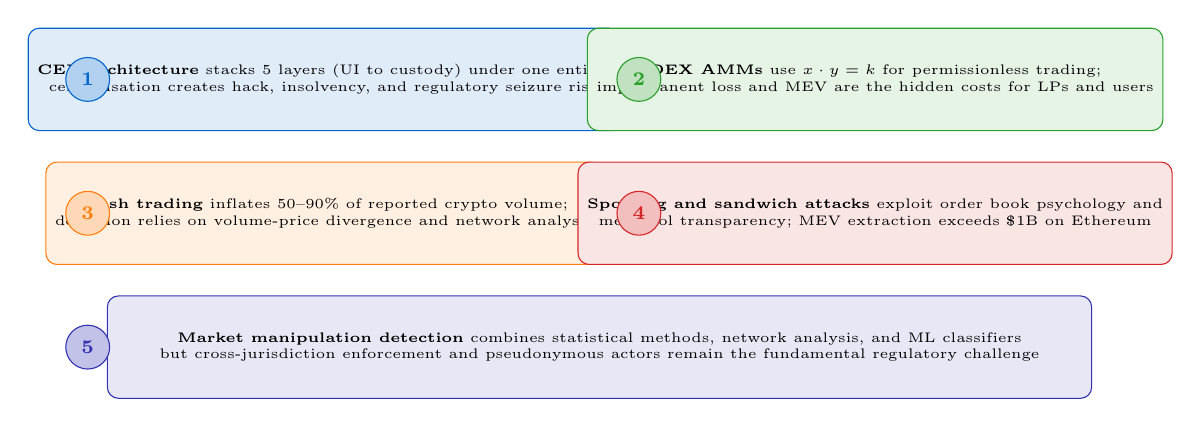
\begin{tikzpicture}
  \node[draw=mlblue, fill=mlblue!12, rounded corners=4pt, minimum width=5.5cm, minimum height=1.3cm, align=center, font=\tiny] (k1) at (4.0,5.0) {\textbf{CEX architecture} stacks 5 layers (UI to custody) under one entity;\\centralisation creates hack, insolvency, and regulatory seizure risk};
  \node[circle, draw=mlblue, fill=mlblue!30, minimum size=0.55cm, font=\scriptsize\bfseries, text=mlblue] at (1.0,5.0) {1};

  \node[draw=mlgreen, fill=mlgreen!12, rounded corners=4pt, minimum width=5.5cm, minimum height=1.3cm, align=center, font=\tiny] (k2) at (11.0,5.0) {\textbf{DEX AMMs} use $x \cdot y = k$ for permissionless trading;\\impermanent loss and MEV are the hidden costs for LPs and users};
  \node[circle, draw=mlgreen, fill=mlgreen!30, minimum size=0.55cm, font=\scriptsize\bfseries, text=mlgreen] at (8.0,5.0) {2};

  \node[draw=mlorange, fill=mlorange!12, rounded corners=4pt, minimum width=5.5cm, minimum height=1.3cm, align=center, font=\tiny] (k3) at (4.0,3.3) {\textbf{Wash trading} inflates 50--90\% of reported crypto volume;\\detection relies on volume-price divergence and network analysis};
  \node[circle, draw=mlorange, fill=mlorange!30, minimum size=0.55cm, font=\scriptsize\bfseries, text=mlorange] at (1.0,3.3) {3};

  \node[draw=mlred, fill=mlred!12, rounded corners=4pt, minimum width=5.5cm, minimum height=1.3cm, align=center, font=\tiny] (k4) at (11.0,3.3) {\textbf{Spoofing and sandwich attacks} exploit order book psychology and\\mempool transparency; MEV extraction exceeds \$1B on Ethereum};
  \node[circle, draw=mlred, fill=mlred!30, minimum size=0.55cm, font=\scriptsize\bfseries, text=mlred] at (8.0,3.3) {4};

  \node[draw=mlpurple, fill=mlpurple!12, rounded corners=4pt, minimum width=12.5cm, minimum height=1.3cm, align=center, font=\tiny] (k5) at (7.5,1.6) {\textbf{Market manipulation detection} combines statistical methods, network analysis, and ML classifiers\\but cross-jurisdiction enforcement and pseudonymous actors remain the fundamental regulatory challenge};
  \node[circle, draw=mlpurple, fill=mlpurple!30, minimum size=0.55cm, font=\scriptsize\bfseries, text=mlpurple] at (1.0,1.6) {5};
\end{tikzpicture}
\bottomnote{Section 4 complete | 5 key takeaways | Proceed to Section 5: Regulation \& Future of Crypto Trading}
\end{frame}

%% ============================================================
%% SECTION 5: REGULATION & FUTURE
%% ============================================================
\section{Regulation \& Future of Crypto Trading}

% Frame 49: Section 5 Divider
\begin{frame}{Section 5: Regulation \& Future of Crypto Trading}
\begin{beamercolorbox}[sep=12pt,center,rounded=true,shadow=true]{palette quaternary}
  {\Large\bfseries Section 5: Regulation \& Future of Crypto Trading}\\[4pt]
  {\normalsize Regulatory frameworks shaping the future of digital asset markets}
\end{beamercolorbox}

\vspace{4mm}
\begin{columns}[T]
\column{0.55\textwidth}
\begin{block}{What You Will Learn}
\begin{itemize}\setlength{\itemsep}{2pt}
  \item Major global regulatory frameworks and their impact on trading
  \item EU MiCA and US SEC/CFTC approaches to crypto markets
  \item Institutional adoption milestones and market structure evolution
  \item Algorithmic trading regulation and the future of crypto markets
\end{itemize}
\end{block}
\column{0.45\textwidth}
\begin{block}{Frames in This Section}
\begin{itemize}\setlength{\itemsep}{2pt}
  \item Frame 50: Global Regulatory Landscape
  \item Frame 51: MiCA Trading Provisions
  \item Frame 52: Institutional Adoption
  \item Frame 53: Algorithmic Trading Regulation
  \item Frame 54: The Future of Crypto Trading
  \item Frame 55: Key Takeaways and Course Summary
\end{itemize}
\end{block}
\end{columns}
\bottomnote{Section 5 of 5 | Frames 49--55 | Regulatory frameworks, institutional adoption, and future market evolution}
\end{frame}

% Frame 50: Global Regulatory Landscape
\begin{frame}{Global Regulatory Landscape}
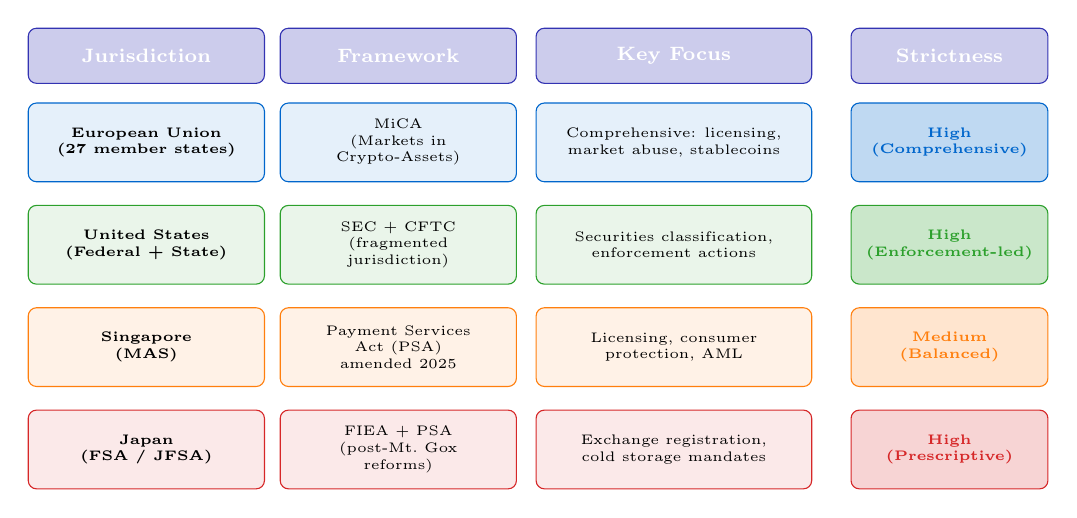
\begin{tikzpicture}
  % Table header
  \node[draw=mlpurple, fill=mlpurple!25, rounded corners=3pt, minimum width=3.0cm, minimum height=0.7cm, align=center, font=\scriptsize\bfseries, text=white] at (1.8,5.8) {Jurisdiction};
  \node[draw=mlpurple, fill=mlpurple!25, rounded corners=3pt, minimum width=3.0cm, minimum height=0.7cm, align=center, font=\scriptsize\bfseries, text=white] at (5.0,5.8) {Framework};
  \node[draw=mlpurple, fill=mlpurple!25, rounded corners=3pt, minimum width=3.5cm, minimum height=0.7cm, align=center, font=\scriptsize\bfseries, text=white] at (8.5,5.8) {Key Focus};
  \node[draw=mlpurple, fill=mlpurple!25, rounded corners=3pt, minimum width=2.5cm, minimum height=0.7cm, align=center, font=\scriptsize\bfseries, text=white] at (12.0,5.8) {Strictness};
  % EU row
  \node[draw=mlblue, fill=mlblue!10, rounded corners=3pt, minimum width=3.0cm, minimum height=1.0cm, align=center, font=\tiny\bfseries] at (1.8,4.7) {European Union\\(27 member states)};
  \node[draw=mlblue, fill=mlblue!10, rounded corners=3pt, minimum width=3.0cm, minimum height=1.0cm, align=center, font=\tiny] at (5.0,4.7) {MiCA\\(Markets in\\Crypto-Assets)};
  \node[draw=mlblue, fill=mlblue!10, rounded corners=3pt, minimum width=3.5cm, minimum height=1.0cm, align=center, font=\tiny] at (8.5,4.7) {Comprehensive: licensing,\\market abuse, stablecoins};
  \node[draw=mlblue, fill=mlblue!25, rounded corners=3pt, minimum width=2.5cm, minimum height=1.0cm, align=center, font=\tiny\bfseries, text=mlblue] at (12.0,4.7) {High\\(Comprehensive)};
  % US row
  \node[draw=mlgreen, fill=mlgreen!10, rounded corners=3pt, minimum width=3.0cm, minimum height=1.0cm, align=center, font=\tiny\bfseries] at (1.8,3.4) {United States\\(Federal + State)};
  \node[draw=mlgreen, fill=mlgreen!10, rounded corners=3pt, minimum width=3.0cm, minimum height=1.0cm, align=center, font=\tiny] at (5.0,3.4) {SEC + CFTC\\(fragmented\\jurisdiction)};
  \node[draw=mlgreen, fill=mlgreen!10, rounded corners=3pt, minimum width=3.5cm, minimum height=1.0cm, align=center, font=\tiny] at (8.5,3.4) {Securities classification,\\enforcement actions};
  \node[draw=mlgreen, fill=mlgreen!25, rounded corners=3pt, minimum width=2.5cm, minimum height=1.0cm, align=center, font=\tiny\bfseries, text=mlgreen] at (12.0,3.4) {High\\(Enforcement-led)};
  % Singapore row
  \node[draw=mlorange, fill=mlorange!10, rounded corners=3pt, minimum width=3.0cm, minimum height=1.0cm, align=center, font=\tiny\bfseries] at (1.8,2.1) {Singapore\\(MAS)};
  \node[draw=mlorange, fill=mlorange!10, rounded corners=3pt, minimum width=3.0cm, minimum height=1.0cm, align=center, font=\tiny] at (5.0,2.1) {Payment Services\\Act (PSA)\\amended 2025};
  \node[draw=mlorange, fill=mlorange!10, rounded corners=3pt, minimum width=3.5cm, minimum height=1.0cm, align=center, font=\tiny] at (8.5,2.1) {Licensing, consumer\\protection, AML};
  \node[draw=mlorange, fill=mlorange!20, rounded corners=3pt, minimum width=2.5cm, minimum height=1.0cm, align=center, font=\tiny\bfseries, text=mlorange] at (12.0,2.1) {Medium\\(Balanced)};
  % Japan row
  \node[draw=mlred, fill=mlred!10, rounded corners=3pt, minimum width=3.0cm, minimum height=1.0cm, align=center, font=\tiny\bfseries] at (1.8,0.8) {Japan\\(FSA / JFSA)};
  \node[draw=mlred, fill=mlred!10, rounded corners=3pt, minimum width=3.0cm, minimum height=1.0cm, align=center, font=\tiny] at (5.0,0.8) {FIEA + PSA\\(post-Mt.\ Gox\\reforms)};
  \node[draw=mlred, fill=mlred!10, rounded corners=3pt, minimum width=3.5cm, minimum height=1.0cm, align=center, font=\tiny] at (8.5,0.8) {Exchange registration,\\cold storage mandates};
  \node[draw=mlred, fill=mlred!20, rounded corners=3pt, minimum width=2.5cm, minimum height=1.0cm, align=center, font=\tiny\bfseries, text=mlred] at (12.0,0.8) {High\\(Prescriptive)};
\end{tikzpicture}
\bottomnote{Global regulatory landscape: EU (MiCA), US (SEC/CFTC), Singapore (MAS), Japan (FSA) | Convergence toward comprehensive frameworks}
\end{frame}

% Frame 51: MiCA Trading Provisions
\begin{frame}{MiCA Trading Provisions}
\begin{columns}[T]
\column{0.50\textwidth}
\begin{block}{Key Provisions}
\begin{itemize}\setlength{\itemsep}{3pt}
  \item \textbf{Market Abuse:} Insider dealing, market manipulation, and unlawful disclosure of inside information prohibited (Title VI)
  \item \textbf{CASP Authorization:} All crypto-asset service providers must obtain authorization from national competent authorities
  \item \textbf{Custody Rules:} Segregation of client assets; CASPs liable for losses including cyber attacks
  \item \textbf{Transparency:} Pre- and post-trade transparency for trading platforms; white paper requirements
  \item \textbf{Stablecoins:} E-money tokens and asset-referenced tokens face reserve and redemption rules
\end{itemize}
\end{block}
\column{0.50\textwidth}
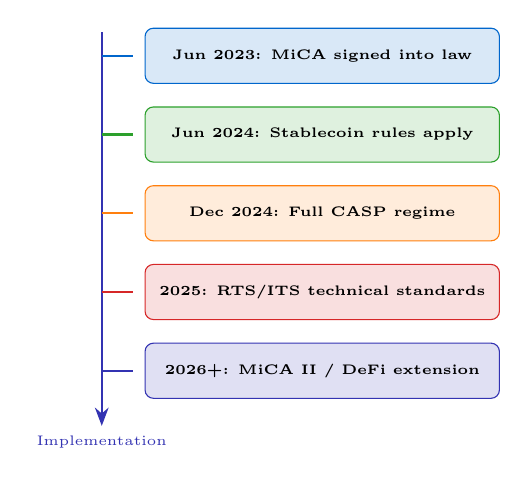
\begin{tikzpicture}
  % Timeline
  \draw[-{Stealth}, thick, mlpurple] (0.0,5.5) -- (0.0,0.5) node[below, font=\tiny] {Implementation};
  % Milestones
  \node[draw=mlblue, fill=mlblue!15, rounded corners=3pt, minimum width=4.5cm, minimum height=0.7cm, align=center, font=\tiny\bfseries] (t1) at (2.8,5.2) {Jun 2023: MiCA signed into law};
  \draw[thick, mlblue] (0.0,5.2) -- (0.4,5.2);
  \node[draw=mlgreen, fill=mlgreen!15, rounded corners=3pt, minimum width=4.5cm, minimum height=0.7cm, align=center, font=\tiny\bfseries] (t2) at (2.8,4.2) {Jun 2024: Stablecoin rules apply};
  \draw[thick, mlgreen] (0.0,4.2) -- (0.4,4.2);
  \node[draw=mlorange, fill=mlorange!15, rounded corners=3pt, minimum width=4.5cm, minimum height=0.7cm, align=center, font=\tiny\bfseries] (t3) at (2.8,3.2) {Dec 2024: Full CASP regime};
  \draw[thick, mlorange] (0.0,3.2) -- (0.4,3.2);
  \node[draw=mlred, fill=mlred!15, rounded corners=3pt, minimum width=4.5cm, minimum height=0.7cm, align=center, font=\tiny\bfseries] (t4) at (2.8,2.2) {2025: RTS/ITS technical standards};
  \draw[thick, mlred] (0.0,2.2) -- (0.4,2.2);
  \node[draw=mlpurple, fill=mlpurple!15, rounded corners=3pt, minimum width=4.5cm, minimum height=0.7cm, align=center, font=\tiny\bfseries] (t5) at (2.8,1.2) {2026+: MiCA II / DeFi extension};
  \draw[thick, mlpurple] (0.0,1.2) -- (0.4,1.2);
\end{tikzpicture}
\end{columns}
\bottomnote{MiCA: first comprehensive crypto regulation | Market abuse, CASP licensing, custody segregation, stablecoin reserves | Full enforcement Dec 2024}
\end{frame}

% Frame 52: Institutional Adoption
\begin{frame}{Institutional Adoption}
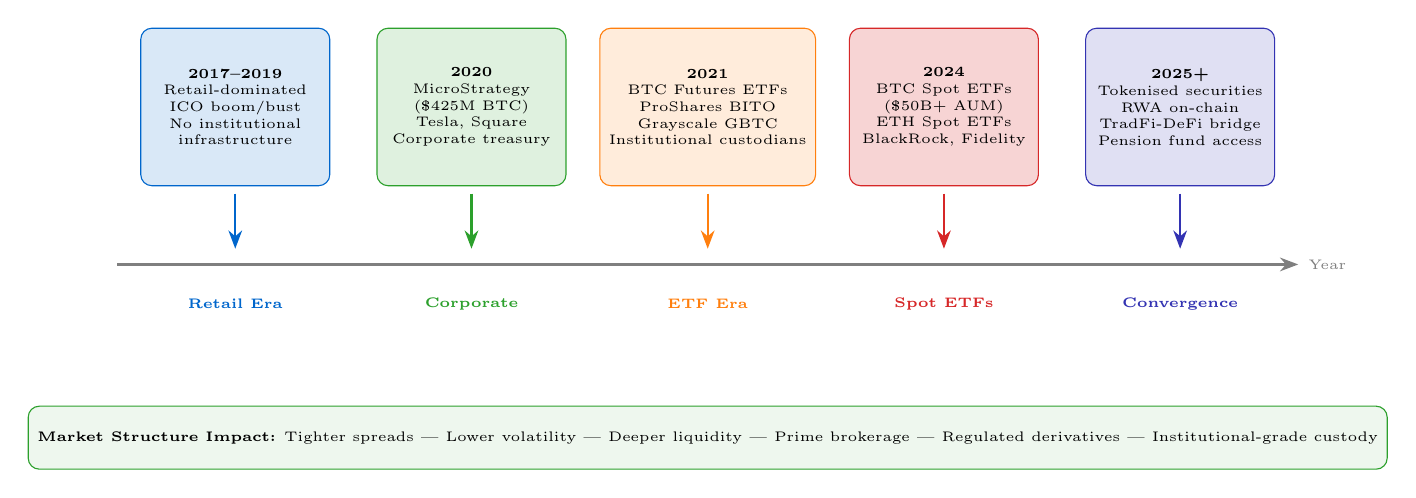
\begin{tikzpicture}
  % Timeline axis
  \draw[-{Stealth}, thick, mlgray] (0.0,3.0) -- (15.0,3.0) node[right, font=\tiny] {Year};
  % 2017 Retail
  \node[draw=mlblue, fill=mlblue!15, rounded corners=4pt, minimum width=2.4cm, minimum height=2.0cm, align=center, font=\tiny] (m1) at (1.5,5.0) {\textbf{2017--2019}\\Retail-dominated\\ICO boom/bust\\No institutional\\infrastructure};
  \draw[-{Stealth}, thick, mlblue] (1.5,3.9) -- (1.5,3.2);
  \node[font=\tiny\bfseries, text=mlblue] at (1.5,2.5) {Retail Era};
  % 2020 Corporate
  \node[draw=mlgreen, fill=mlgreen!15, rounded corners=4pt, minimum width=2.4cm, minimum height=2.0cm, align=center, font=\tiny] (m2) at (4.5,5.0) {\textbf{2020}\\MicroStrategy\\(\$425M BTC)\\Tesla, Square\\Corporate treasury};
  \draw[-{Stealth}, thick, mlgreen] (4.5,3.9) -- (4.5,3.2);
  \node[font=\tiny\bfseries, text=mlgreen] at (4.5,2.5) {Corporate};
  % 2021 ETFs
  \node[draw=mlorange, fill=mlorange!15, rounded corners=4pt, minimum width=2.4cm, minimum height=2.0cm, align=center, font=\tiny] (m3) at (7.5,5.0) {\textbf{2021}\\BTC Futures ETFs\\ProShares BITO\\Grayscale GBTC\\Institutional custodians};
  \draw[-{Stealth}, thick, mlorange] (7.5,3.9) -- (7.5,3.2);
  \node[font=\tiny\bfseries, text=mlorange] at (7.5,2.5) {ETF Era};
  % 2024 Spot ETFs
  \node[draw=mlred, fill=mlred!20, rounded corners=4pt, minimum width=2.4cm, minimum height=2.0cm, align=center, font=\tiny] (m4) at (10.5,5.0) {\textbf{2024}\\BTC Spot ETFs\\(\$50B+ AUM)\\ETH Spot ETFs\\BlackRock, Fidelity};
  \draw[-{Stealth}, thick, mlred] (10.5,3.9) -- (10.5,3.2);
  \node[font=\tiny\bfseries, text=mlred] at (10.5,2.5) {Spot ETFs};
  % 2025+ Future
  \node[draw=mlpurple, fill=mlpurple!15, rounded corners=4pt, minimum width=2.4cm, minimum height=2.0cm, align=center, font=\tiny] (m5) at (13.5,5.0) {\textbf{2025+}\\Tokenised securities\\RWA on-chain\\TradFi-DeFi bridge\\Pension fund access};
  \draw[-{Stealth}, thick, mlpurple] (13.5,3.9) -- (13.5,3.2);
  \node[font=\tiny\bfseries, text=mlpurple] at (13.5,2.5) {Convergence};
  % Impact bar
  \node[draw=mlgreen, fill=mlgreen!8, rounded corners=4pt, minimum width=14.0cm, minimum height=0.8cm, align=center, font=\tiny] at (7.5,0.8) {%
    \textbf{Market Structure Impact:} Tighter spreads | Lower volatility | Deeper liquidity | Prime brokerage | Regulated derivatives | Institutional-grade custody};
\end{tikzpicture}
\bottomnote{Institutional adoption timeline: retail (2017) to spot ETFs (2024) to tokenised securities (2025+) | Each milestone compresses spreads and deepens liquidity}
\end{frame}

% Frame 53: Algorithmic Trading Regulation
\begin{frame}{Algorithmic Trading Regulation}
\begin{columns}[T]
\column{0.50\textwidth}
\begin{block}{TradFi: MiFID II Requirements}
\begin{itemize}\setlength{\itemsep}{3pt}
  \item \textbf{Authorization:} Algo firms must register and maintain capital
  \item \textbf{Kill Switches:} Mandatory circuit breakers to halt runaway algos
  \item \textbf{Risk Limits:} Pre-trade checks on price, size, and credit
  \item \textbf{Testing:} Backtesting and stress testing in sandbox before live
  \item \textbf{Record Keeping:} Full order audit trail retained 5+ years
  \item \textbf{Market Making:} Obligations to provide liquidity continuously
\end{itemize}
\end{block}
\vspace{2mm}
\begin{alertblock}{Key Gap}
\scriptsize Most crypto exchanges have no algo trading regulations. Flash crashes (e.g., BTC $-$87\% on Binance.US, 2021) occur without circuit breakers.
\end{alertblock}
\column{0.50\textwidth}
\begin{block}{Crypto: Emerging Requirements}
\begin{itemize}\setlength{\itemsep}{3pt}
  \item \textbf{MiCA Art.\ 76--80:} Market abuse rules apply to algo trading
  \item \textbf{No Kill Switch Mandate:} Most DEXs have no halt mechanism
  \item \textbf{MEV Regulation:} Not yet addressed in any framework
  \item \textbf{DeFi Bots:} Autonomous smart contracts outside legal scope
  \item \textbf{Cross-Border:} Jurisdiction arbitrage by algo operators
\end{itemize}
\end{block}
\vspace{2mm}
\begin{block}{Future: Convergence Path}
\begin{itemize}\setlength{\itemsep}{3pt}
  \item Kill switches for CASPs under MiCA II
  \item Pre-trade risk controls for API traders
  \item MEV-specific regulation (EIP proposals)
  \item On-chain algo registration requirements
  \item Unified TradFi-crypto surveillance
\end{itemize}
\end{block}
\end{columns}
\bottomnote{Algo trading regulation: TradFi (MiFID II) mature vs crypto (MiCA) emerging | Convergence expected via kill switches, risk controls, and MEV rules}
\end{frame}

% Frame 54: The Future of Crypto Trading
\begin{frame}{The Future of Crypto Trading}
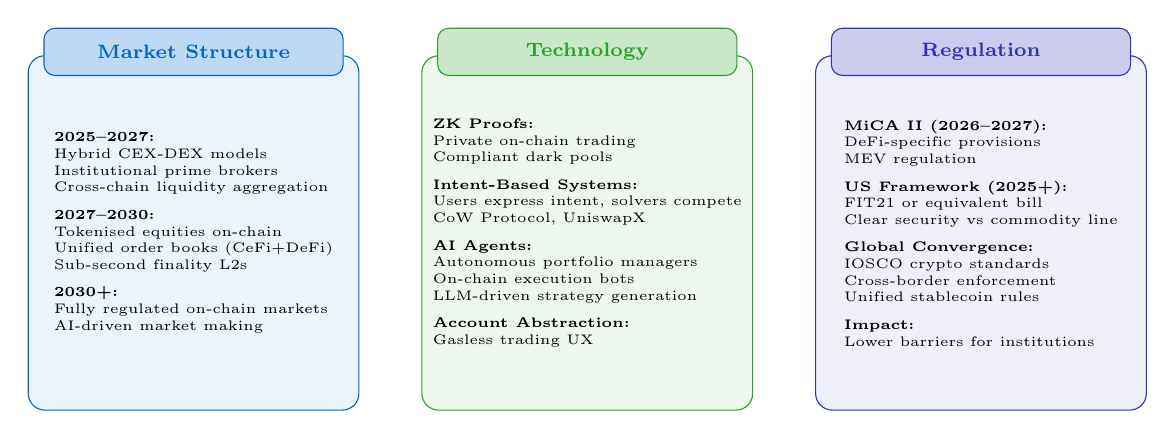
\begin{tikzpicture}
  % Panel 1: Market Structure Evolution
  \node[draw=mlblue, fill=mlblue!8, rounded corners=6pt, minimum width=4.2cm, minimum height=4.5cm, align=center] at (2.5,3.2) {};
  \node[draw=mlblue, fill=mlblue!25, rounded corners=4pt, minimum width=3.8cm, minimum height=0.6cm, align=center, font=\scriptsize\bfseries, text=mlblue] at (2.5,5.5) {Market Structure};
  \node[align=left, font=\tiny] at (2.5,3.2) {%
    \textbf{2025--2027:}\\
    Hybrid CEX-DEX models\\
    Institutional prime brokers\\
    Cross-chain liquidity aggregation\\[4pt]
    \textbf{2027--2030:}\\
    Tokenised equities on-chain\\
    Unified order books (CeFi+DeFi)\\
    Sub-second finality L2s\\[4pt]
    \textbf{2030+:}\\
    Fully regulated on-chain markets\\
    AI-driven market making};
  % Panel 2: Technology Convergence
  \node[draw=mlgreen, fill=mlgreen!8, rounded corners=6pt, minimum width=4.2cm, minimum height=4.5cm, align=center] at (7.5,3.2) {};
  \node[draw=mlgreen, fill=mlgreen!25, rounded corners=4pt, minimum width=3.8cm, minimum height=0.6cm, align=center, font=\scriptsize\bfseries, text=mlgreen] at (7.5,5.5) {Technology};
  \node[align=left, font=\tiny] at (7.5,3.2) {%
    \textbf{ZK Proofs:}\\
    Private on-chain trading\\
    Compliant dark pools\\[4pt]
    \textbf{Intent-Based Systems:}\\
    Users express intent, solvers compete\\
    CoW Protocol, UniswapX\\[4pt]
    \textbf{AI Agents:}\\
    Autonomous portfolio managers\\
    On-chain execution bots\\
    LLM-driven strategy generation\\[4pt]
    \textbf{Account Abstraction:}\\
    Gasless trading UX};
  % Panel 3: Regulatory Clarity
  \node[draw=mlpurple, fill=mlpurple!8, rounded corners=6pt, minimum width=4.2cm, minimum height=4.5cm, align=center] at (12.5,3.2) {};
  \node[draw=mlpurple, fill=mlpurple!25, rounded corners=4pt, minimum width=3.8cm, minimum height=0.6cm, align=center, font=\scriptsize\bfseries, text=mlpurple] at (12.5,5.5) {Regulation};
  \node[align=left, font=\tiny] at (12.5,3.2) {%
    \textbf{MiCA II (2026--2027):}\\
    DeFi-specific provisions\\
    MEV regulation\\[4pt]
    \textbf{US Framework (2025+):}\\
    FIT21 or equivalent bill\\
    Clear security vs commodity line\\[4pt]
    \textbf{Global Convergence:}\\
    IOSCO crypto standards\\
    Cross-border enforcement\\
    Unified stablecoin rules\\[4pt]
    \textbf{Impact:}\\
    Lower barriers for institutions};
\end{tikzpicture}
\bottomnote{Three pillars of crypto trading evolution: market structure convergence, technology innovation (ZK, intents, AI), regulatory clarity (MiCA II, FIT21)}
\end{frame}

% Frame 55: Key Takeaways and Course Summary
\begin{frame}{Key Takeaways and Course Summary}
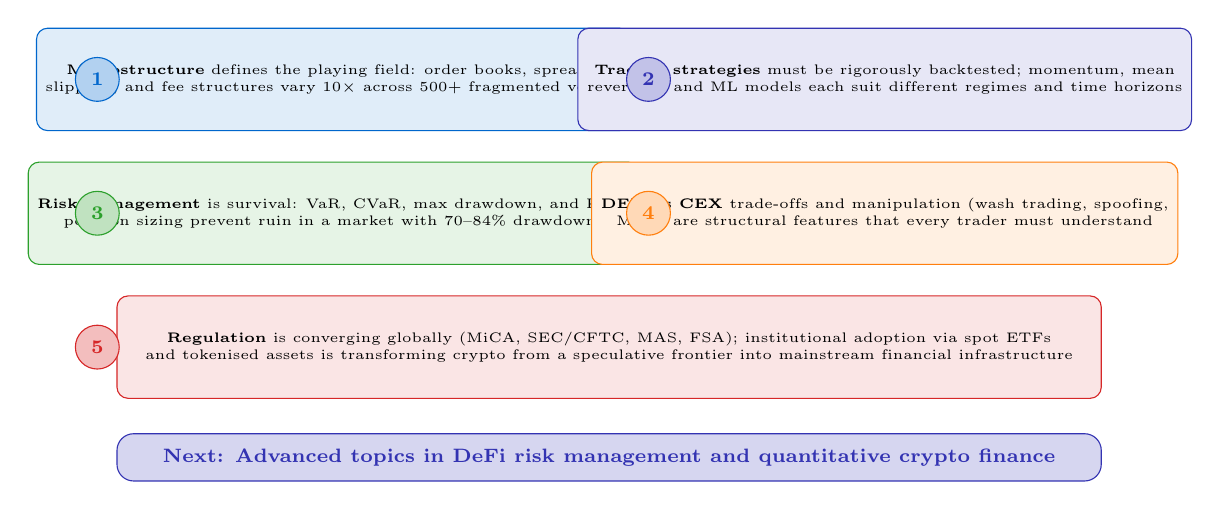
\begin{tikzpicture}
  \node[draw=mlblue, fill=mlblue!12, rounded corners=4pt, minimum width=5.5cm, minimum height=1.3cm, align=center, font=\tiny] (k1) at (4.0,5.0) {\textbf{Microstructure} defines the playing field: order books, spreads,\\slippage, and fee structures vary 10$\times$ across 500+ fragmented venues};
  \node[circle, draw=mlblue, fill=mlblue!30, minimum size=0.55cm, font=\scriptsize\bfseries, text=mlblue] at (1.0,5.0) {1};

  \node[draw=mlpurple, fill=mlpurple!12, rounded corners=4pt, minimum width=5.5cm, minimum height=1.3cm, align=center, font=\tiny] (k2) at (11.0,5.0) {\textbf{Trading strategies} must be rigorously backtested; momentum, mean\\reversion, and ML models each suit different regimes and time horizons};
  \node[circle, draw=mlpurple, fill=mlpurple!30, minimum size=0.55cm, font=\scriptsize\bfseries, text=mlpurple] at (8.0,5.0) {2};

  \node[draw=mlgreen, fill=mlgreen!12, rounded corners=4pt, minimum width=5.5cm, minimum height=1.3cm, align=center, font=\tiny] (k3) at (4.0,3.3) {\textbf{Risk management} is survival: VaR, CVaR, max drawdown, and Kelly\\position sizing prevent ruin in a market with 70--84\% drawdowns};
  \node[circle, draw=mlgreen, fill=mlgreen!30, minimum size=0.55cm, font=\scriptsize\bfseries, text=mlgreen] at (1.0,3.3) {3};

  \node[draw=mlorange, fill=mlorange!12, rounded corners=4pt, minimum width=5.5cm, minimum height=1.3cm, align=center, font=\tiny] (k4) at (11.0,3.3) {\textbf{DEX vs CEX} trade-offs and manipulation (wash trading, spoofing,\\MEV) are structural features that every trader must understand};
  \node[circle, draw=mlorange, fill=mlorange!30, minimum size=0.55cm, font=\scriptsize\bfseries, text=mlorange] at (8.0,3.3) {4};

  \node[draw=mlred, fill=mlred!12, rounded corners=4pt, minimum width=12.5cm, minimum height=1.3cm, align=center, font=\tiny] (k5) at (7.5,1.6) {\textbf{Regulation} is converging globally (MiCA, SEC/CFTC, MAS, FSA); institutional adoption via spot ETFs\\and tokenised assets is transforming crypto from a speculative frontier into mainstream financial infrastructure};
  \node[circle, draw=mlred, fill=mlred!30, minimum size=0.55cm, font=\scriptsize\bfseries, text=mlred] at (1.0,1.6) {5};

  % Teaser bar
  \node[draw=mlpurple, fill=mlpurple!20, rounded corners=6pt, minimum width=12.5cm, minimum height=0.6cm, align=center, font=\scriptsize\bfseries, text=mlpurple] at (7.5,0.2) {Next: Advanced topics in DeFi risk management and quantitative crypto finance};
\end{tikzpicture}
\bottomnote{Course complete | 5 sections, 55 frames | From microstructure to regulation: a quantitative framework for crypto trading}
\end{frame}

\end{document}
